\documentclass[algorithmlist,figurelist,tablelist,nomlist,engineer]{seumasterthesis}
\usepackage{setspace}
\begin{document}

%% ----------------------------------------------------------------------------
%%                                 Meta Data
%% ---------------------RR-------------------------------------------------------
\categorynumber{TP15}           % Chinese Library Classification
\UDC{001.9}                     % Universal Decimal Classification
\secretlevel{公开}                % Secret Level
\studentid{170001}              % Student Number

%% ----------------------------------------------------------------------------
%%                           Thesis Title and Spine
%% ----------------------------------------------------------------------------
\title
    {ASP程序的解释与调试}                                      % Thesis Title
    {系统的设计与实现}                                          % Thesis Subtitle
    {Design and Implementation of}  % Thesis English Title
    {Explanation and Debugging System for ASP Program}            % Thesis English Subtitle

\spine
    {ASP程序的解释与调试 \rotatebox{270}{\raisebox{2.5pt}{LaTeX}} 论文模板使用手册}      % Spine Title
    {}                                                          % Spine Subtitle

%% ----------------------------------------------------------------------------
%%                             Author and Advidor
%% ----------------------------------------------------------------------------
\author
    {胡闰秋}                        % Author Name in Chinese
    {HU Runqiu}                 % Author Name in English

\advisor
    {张志政\ \ 副教授}                       % Advisor Name (Chinese)
    {ZHANG Zhi-zheng}           % Advisor Name (English)
    {Associate Prof.}                     % Advisor Title (English)

% \coadvisor
%     {程光}                        % Co-advisor Name (Chinese)
%     {CHENG Guang}               % Co-advisor Name (English)
%     {Prof.}                     % Co-advisor Title (English)

%% ----------------------------------------------------------------------------
%%                              Thesis Defence
%% ----------------------------------------------------------------------------
\engthesistype{应用研究}            % Engineering Master Thesis Type
\degreetype                     % Degree Type
    {工程硕士}
    {Master of Engineering}
\major{计算机技术(专业学位)}                  % First-level Discipline Name
\submajor{}               % Second-level Discipline Name
\defenddate{2021年6月x日}         % Defence Date
\authorizedate{2021年6月x日}      % Degree Award Date
\committeechair{不知道1}             % Chairman of Defence Committee
\reviewer{不知道2}{不知道3}             % Thesis Reviewer(s)
\department                     % Faculty or Department
    {计算机科学与工程学院}
    {School of Computer Science and Engineering}
\seuthesisthanks                % Short Acknowledgement
    {本文的部分工作受国家自然基金 No. xxxxxx 的支持与帮助,在此表示感谢。}

%% ----------------------------------------------------------------------------
%%                                  Cover
%% ----------------------------------------------------------------------------
\makebigcover
\makecover
	
%% ----------------------------------------------------------------------------
%%                          Abstract and Contents
%% ----------------------------------------------------------------------------
%% ----------------------------------------------------------------------------
%%                              Chinese Abstract
%% ----------------------------------------------------------------------------

\begin{abstract}{回答集程序,逻辑程序解释发现,逻辑程序调试}
% \thispagestyle{zhcnabstract}
本文提出了一个新的东南大学
\end{abstract}

%% ----------------------------------------------------------------------------
%%                              English Abstract
%% ----------------------------------------------------------------------------
\begin{englishabstract}{Answer Set Programming, Explanation Finding for Logic Programs, Debugging for Logic Programs}
This article proposes a new Southeast University master degree thesis
\end{englishabstract}

\begin{spacing}{1.2}
\tableofcontents
\end{spacing}
\listofothers

%% ----------------------------------------------------------------------------
%%                                Main Body
%% ----------------------------------------------------------------------------
\mainmatter
\chapter{绪论}
\label{chp:introsuction}
\nomtypeG{ASP}{Answer Set Programming}{回答集程序}
\nomtypeG{GDPR}{General Data \\Protection Regulation}{通用数据保护准则}
\nomtypeG{DARPA}{Defense Advanced\\ Research Projects Agency}{美国国防部\\高级研究计划局}
\nomtypeG{ABA}{Assumption-based Argumentation}{基于假设的论证}
\nomtypeG{LABAS}{Labelled ABA-based Answer Set}{有标签的基于ABA的回答集}
\nomtypeG{NAF}{Negation As Failure}{失败即否定}
\nomtypeG{NLP}{Normal Logic Program}{一般逻辑程序}
\nomtypeG{IDE}{Integrated Development Environment}{集成开发环境}


\section{研究背景与动机}
随着人工智能技术的高速发展,基于人工智能技术的解决方案正在被各行各业普遍应用。与此同时,人工智能所做出的决策是否合法合规、值得信赖的问题引发人们的探讨,对人工智能可解释性的研究开始受到国内外的广泛关注。2021年3月,十三届全国人大四次会议通过《中华人民共和国国民经济和社会发展第十四个五年规划和2035年远景目标纲要》\cite{guowuyuan2021shisiwu},其中科技前沿领域攻关目标中提出了新一代人工智能学习推理与决策创新的要求;2017年10月,国务院印发的《新一代人工智能发展规划》\cite{guowuyuan2017aiplan}中更具体地指出要进一步研究不确定性推理与决策,机器直觉推理与因果模型等基础理论,同时提出了实现具备高可解释性、强泛化能力的人工智能的目标。2016年10月,美国DARPA实验室启动可解释的人工智能(eXplainableAI,XAI)项目\cite{gunning2017explainable} ,提出建立一套改进的机器学习技术生成可解释的模型,结合有效的解释技术,使得最终用户能够理解人工智能系统的目标;欧盟在2016年颁布的通用数据保护规范(GDPR\cite{regulation2016regulation} )中提出,“任何人都有权利拒绝接受仅基于机器处理得到的涉及重大个人利益的决策”,所有决策只有具备解释才会为人接受\cite{goodman2017european}。由此可见,解释在人工智能领域研究中越来越受到关注。

回答集编程(Answer Set Programming,ASP)是一种流行的用于决策和解决问题的人工智能编程范式。作为一种声明式语言,ASP程序作为具有强大的表达力,并已被成功用于多个领域\cite{erdem2016applications},例如生物学\cite{erdem2015generating}、心理学\cite{psychology2010Balduccini}、医学\cite{bao2011medical, zhang2014preliminary}、机器人家庭服务\cite{jjm2010robertasp}以及音乐创作\cite{boennAutomaticMusicComposition2011}等。使用ASP求解问题的主要优势是程序编写结构紧凑,编写速度很快,程序员可以专注于对问题的描述而不必关心搜索算法的具体设计,搜索求解的工作统一由各种求解器完成\cite{brain2008answer}。然而,这一优势的背后意味着ASP程序的推理求解对使用者而言是一个“黑盒”\cite{huaqi2018lp}。在求解过程中,用户无法得知答案是如何一步步推理得到的。当求解结果与个人认知不一致时,需要对推理结果进行完整、准确的解释。因此,有必要建立一个面向ASP程序的解释模型。另一方面,从ASP编程人员的角度看,当程序执行结果与预期不一致时,为了明确程序编写中是否存在问题,需要对程序进行调试。现有的实际应用中,对ASP程序进行调试通常是采用人工对程序中的规则和原子逐一检查的方式进行的,这一过程耗费了大量时间和精力\cite{dodaroInteractiveDebuggingNonground2015}。当程序规模不断增大时,调试的难度也随之上升。而在命令式编程语言(如Python,Java,C++等)中,通过设置断点、单步调试、观察变量值等与用户交互的调试方式,可以有效地发现程序中的问题\cite{stumptner1998survey}。在ASP程序的编写和调试中引入这种调试模式,辅助检查ASP程序中的语法和语义错误,能够有效降低ASP程序的学习门槛,节约开发过程中的时间成本,有助于推广ASP程序在工程中更广泛的应用。

综上,设计实现一个可交互的ASP程序解释和调试系统,在提升决策可解释性,增强开发效率方面具有重要的工程研究价值。本文针对上述对ASP程序进行解释和调试的实际需求,首先构建ASP程序解释模型,并基于该解释模型提出ASP程序的调试模型,在解释和调试模型的基础上,设计实现一个面向用户的交互式ASP程序解释和调试系统。
\section{相关研究现状}
当前,对ASP程序的解释,国内外的研究可分为对一致性ASP程序的解释和非一致性ASP程序的解释。其中,对一致性ASP程序的解释,也称为理由(justification),对非一致性ASP程序的解释,现有研究中认为就是ASP程序的调试(debugging)\cite{fandAnsWhy2019}。因此本节按照上述分类,分两部分介绍当前国内外研究现状。

\subsection{对一致性ASP程序的解释}
对一致性ASP程序的解释,按照解释呈现的形式又可以分为三类:基于文字与规则依赖图的解释,基于命题公式的解释和基于规则集的解释。Pontelli等人在\cite{pontelli2006justifications, pontelli2009justifications}中提出了离线解释(Off-line Justification)的概念。离线解释是描述某一回答集下原子真值的推导过程的图结构,其中每个顶点代表一个原子,每个边代表其连接的两个原子通过程序中某个规则形成的关联,由规则头部原子指向体部中的某个原子。花琪等人参考已有的关于ASP程序的图表示的方法\cite{albrecht2014construction,linke2005suitable},定义了以与或图为基础的ASP程序解释空间\cite{huaqi2018lp},该空间以程序中的规则与文字作为结点,通过边来表示其之间的依赖关系,最终将某一文字推理解释定义为解释空间的无环子图。这种解释方式与离线解释的最大不同在于将规则显式地引入了图中,而不仅是表示文字之间的依赖关系。可以看到,无论是否包含规则结点,上述解释中,使得某文字为真的每一步推导都包含在解释图中。与这种方式不同,Schulz等人基于论证(argumentation)理论提出LABAS解释\cite{schulz2013argumentationbased,schulz2016justifying},将推导中使用到的中间规则抽象出来,只展示待解释的文字以及推导过程中的出现的事实与规则的负体部,同时对否定文字$not\ l$的真值解释不再基于假设,而是通过对其肯定形式$l$的真值进行解释来呈现。除了上述两种由程序与回答集直接构建文字-规则依赖图的解释方式外,Cabalar等人还提出了基于因果推理的因果解释图,并在一系列工作中分别实现了不含失败即否定(Negation As Failure,NAF)文字的一般逻辑程序(Normal Logic Program,NLP)、含有NAF的NLP以及头部含有认知析取的逻辑程序的因果图解释\cite{albrecht2014construction,cabalar2016justificationsa,cabalar2017enablers}。由于因果推理本身就是一种形式化的推理方法,因此这种方式的解释能够很好地将推理过程中的语义信息在解释图中呈现。每一个回答集中的文字都对应着一个因果值集合,用于解释回答集包含该文字的原因。不同于基于图的解释,Carlos等人采用了声明式逻辑方法,基于良基模型(Well-founded Model)对NLP中原子的真值进行解释,最终以命题公式的形式呈现,被称为why-not解释\cite{viegasdamasio2013justifications}。除此之外,Bertaix等人从规则的角度出发研究逻辑程序解释的概念,其研究认为回答集计算的固有猜测应当是针对规则的适用性进行猜测,而非原子真值。因此,其解释呈现的形式为一系列规则组成的集合\cite{beatrix2016justifications}。除了上述从规则和(或)文字的角度进行解释的方法以外,还有少部分研究着眼于证明的形式化的理论\cite{denecker1993justification,denecker2015formal}。在这种理论下,每个程序都引入了一种“证明框架”的语义结构,用于说明该程序某结论正确的潜在原因。不过,与综述的其他方法不同,这些工作侧重于将证明的概念作为数学工具来理解不同的语义(并提出新的语义),而不是以一种紧凑的方式来回答为什么得出某结论的手段。表\ref{tbl:review_exp}总结了上述文献中的各种对一致性程序的解释方法及相关解释示例,并对应给出了本文所提出的解释的各要素说明。要说明的是,表中所有的示例均基于下面的程序$P_1$:
$$r_1: p \leftarrow t \land not\ q \qquad\qquad r_2: q \leftarrow s \qquad\qquad r_3: s \leftarrow not\ p \qquad\qquad r_4: t$$%
该程序有两个回答集,$M_1=\{t,s,q\}$,$M_2=\{t, p\}$。表\ref{tbl:review_exp}中的样例展示的是原子$p$在回答集$M_2$下的解释。可以看到,本文的解释在支持的程序类型、推导过程的展示、对否定文字的解释方式上均进行了改进。其中,支持的程序类型中关注到了ASP领域内常用到的选择规则,同时考虑了非实例化程序的实例化处理。另外,在推导过程的展示以及对否定文字的解释中还引入了用户交互。
\begin{sidewaystable}
    \caption{已有一致性程序解释工作总结与本文对比}\label{tbl:review_exp}
    \begin{adjustbox}{scale=0.55,center}
    \centering
    \semiLarge
    \setlength{\tabcolsep}{3mm}{
    \begin{tabular}{ m{0.15\textwidth}  m{0.15\textwidth}  m{0.1\textwidth} m{0.1\textwidth}  m{0.15\textwidth} m{0.12\textwidth}  m{0.1\textwidth} m{0.1\textwidth}  m{0.15\textwidth} m{0.25\textwidth}  }
      \hline
      \makecell{\textbf{解释方法}} & \makecell{\textbf{程序类型}} & \makecell{\textbf{解释角度}} & \makecell{\textbf{推导过程}} & \makecell{\textbf{解释对象}} &\makecell{\textbf{使用的}\\\textbf{其他模型}\footnote[1]{除稳定模型语义外的模型}} & \makecell{\textbf{否定文字}} & \makecell{\textbf{无限解释}} & \makecell{\textbf{无穷多个解释}} & \makecell{\textbf{解释结果示意}\\\textbf{(以}$P_1$\textbf{为例)}} \\ \hline
      \makecell{\textbf{离线解释}\cite{pontelli2006justifications,pontelli2009justifications}} & \makecell{NLP} & \makecell{文字依赖} & \makecell{完全包含} &\makecell{文字是否\\在回答集} & \makecell{良基语义} & \makecell{假设或进\\一步解释} & \makecell{有限程序\\不会出现} & \makecell{有限程序\\不会出现} &  \makecell{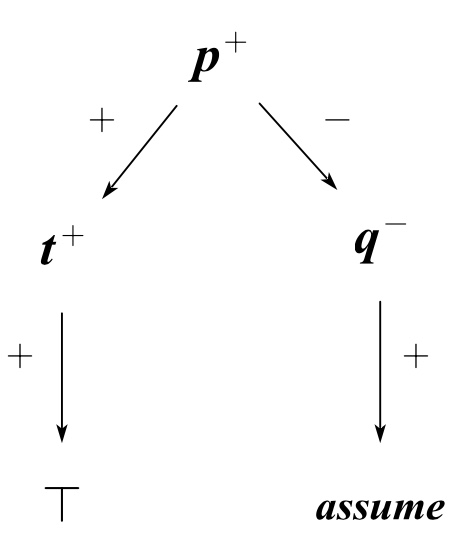
\includegraphics[scale=0.25,trim=0 0 0 -5]{figures/exp_1.jpg}}\\ 
      \makecell{\textbf{LABAS解释}\cite{schulz2013argumentationbased,schulz2016justifying}} & \makecell{含强否\\定的NLP} & \makecell{文字依赖} & \makecell{部分包含} &\makecell{文字是否\\在回答集} & \makecell{-} & \makecell{进一步解释} & \makecell{存在} & \makecell{存在} &  \makecell{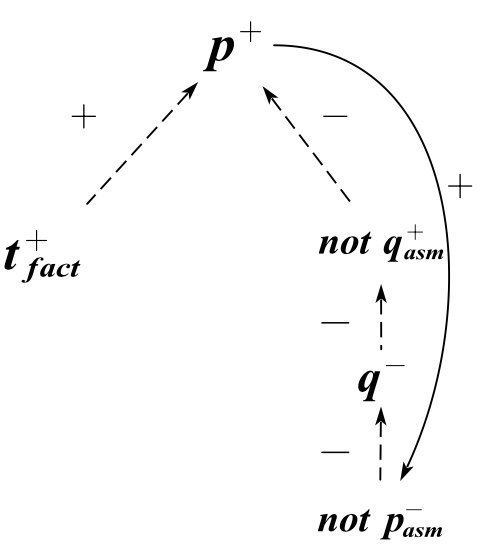
\includegraphics[scale=0.25,trim=0 0 0 -5]{figures/exp_2.jpg}}\\
      \makecell{\textbf{因果图解释}\cite{albrecht2014construction,cabalar2016justificationsa,cabalar2017enablers}} & \makecell{含强否定与\\嵌套表达式\\的NLP} & \makecell{规则-文字\\依赖} & \makecell{完全包含} &\makecell{文字在\\回答集} & \makecell{-} & \makecell{基于假设} & \makecell{有限程序\\不会出现} & \makecell{有限程序\\不会出现} &  \makecell{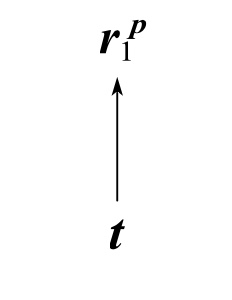
\includegraphics[scale=0.25,trim=0 0 0 -5]{figures/exp_3.jpg}}\\
      \makecell{\textbf{基本解释}\cite{huaqi2018lp}} & \makecell{NLP} & \makecell{规则-文字\\依赖} & \makecell{完全包含} &\makecell{文字在\\回答集} & \makecell{-} & \makecell{未做解释} & \makecell{有限程序\\不会出现} & \makecell{有限程序\\不会出现} &  \makecell{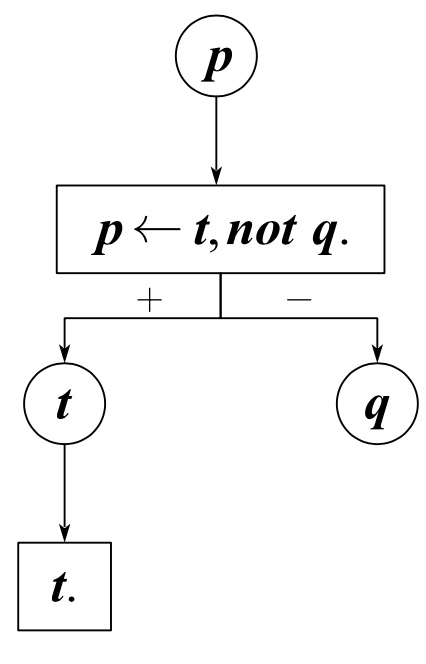
\includegraphics[scale=0.25,trim=0 0 0 -5]{figures/exp_4.jpg}}\\
      \makecell{\textbf{why-not解释}\cite{viegasdamasio2013justifications}} & \makecell{NLP} & \makecell{规则依赖} & \makecell{完全包含} &\makecell{文字是否属于\\完全良基模型} & \makecell{无需回答集} & \makecell{进一步解释} & \makecell{有限程序\\不会出现} & \makecell{有限程序\\不会出现} &  \makecell{$r_1 \land t \land\ not(q) \land \lnot r_3$} \\[5ex]
      \makecell{\textbf{基于规则解释}\cite{beatrix2016justifications}} & \makecell{NLP} & \makecell{规则依赖} & \makecell{完全包含} &\makecell{文字是否\\在回答集} & \makecell{-} & \makecell{进一步解释} & \makecell{有限程序\\不会出现} & \makecell{有限程序\\不会出现} &  \makecell{$\{r_1,t\}$}\\[5ex]
      \makecell{\textbf{形式理论解释}\cite{denecker1993justification,denecker2015formal}} & \makecell{NLP} & \makecell{文字依赖} & \makecell{完全包含} &\makecell{整个回答集} & \makecell{-} & \makecell{进一步解释} & \makecell{存在} & \makecell{有限程序\\不会出现} &  \makecell{$p \rightarrow t$\\$p \rightarrow not\ q \rightarrow not\ s \rightarrow p \rightarrow \ldots$}\\[5ex]
      \makecell{\textbf{本文}} & \makecell{含选择规则\\强否定的\\非实例化NLP\footnote[2]{上述其他研究均未考虑对程序实例化的处理}} & \makecell{规则-文字\\依赖} & \makecell{通过交互\\部分呈现} &\makecell{文字是否\\在回答集} & \makecell{良基语义} & \makecell{通过交互\\进行解释} & \makecell{有限程序\\不会出现} & \makecell{有限程序\\不会出现} &  \makecell{详见后文\\实验结果}\\
      \hline\\
    \end{tabular}}
\end{adjustbox}
\end{sidewaystable}
\subsection{对不一致ASP程序的调试}
对于不一致的 ASP 程序,现有的调试技术主要有如下三种类别:基于标签(元程序)技术、基于诊断技术和基于依赖图的方式\cite{dfj2012jiyuqifash}。前两种技术给出造成程序不一致的集合,但不能够清晰地体现集合之间的关系,以及错误产生的底层原因。最后一种方法是基于支撑原因分析图的调试方法,该方法不仅可以以图的形式直观地给出程序中的错误,还可以给出错误来源及其相互间联系,从而为ASP程序调试提供更为强大的支撑。

Brain等人从Lin等人给出的\cite{lin2004assat}、由Jooyung Lee等人进一步扩展\cite{lee2005modeltheoretic}得到的回答集的定义角度出发,通过找到违背定义中的某一条原则,为程序$P$的每条规则的满足与不满足情况进行元程序规则的编写,能够用于说明某一原子为何不在一个一致性程序的回答集中,也能够用于为不一致程序生成潜在的回答集并指出为何该回答集不能满足程序的规则,进而解释程序不一致的原因,这一工作最终被集成在\textsf{SPOCK}平台中\cite{brain2007that,brain2007debugging}。SPOCK在调试中未能处理非实例化的问题,因此在\textsf{SPOCK}的基础上,Ostsch等人开发了能够处理包含变量的扩展逻辑程序的调试工具\textsf{Ouroboros}\cite{oetsch2010catching}。Polleres等人进一步扩展\textsf{Ouroboros}\cite{polleres2013debugging}来处理程序中的选择规则、基数以及弱约束\cite{calimeri2020aspcore2},最终由Fr\"uhst\"uck等人将该上述工作整合进入ASP集成开发环境(Integrated Development Environment,IDE)中,称为SeaLion IDE\cite{fruhstuck2013debugging}。

上述一系列工作存在一个显著的问题,调试生成的符号信息在数量上可能会非常庞大。\textsf{Ouro-boros}通过要求用户声明一个意向的回答集来缩减规模,但对于不一致程序而言,用户可能无法声明出这样一个回答集。于是,第二类调试技术——引入用户交互的调试应运而生,这一系列技术提出诊断(diagnosis)的概念。其中Shchekotykhin在\textsf{SPOCK}的基础上通过询问逐个用户某一原子atom是否应该出现在回答集中并根据用户的答案缩减调试的规模,同时减少用户声明整个回答集的负担\cite{shchekotykhin2015interactive}。Dodaro\cite{dodaro2015interactive}和Gasteiger\cite{gasteiger2016integrated}在此基础上,实现了对于非实例化程序的调试,通过计算无法满足核心(unsatisfiable core),基于ASP求解器WASP\cite{alviano2013wasp,alviano2015advances}的求解过程来寻找程序的不一致性所在。

最后一类调试技术以Oetsch和P\"uhrer等人的一系列工作为代表\cite{oetsch2011stepping,oetsch2018stepwise,puhrer2014stepwise},以抽象约束程序为基础,对ASP程序使用类似于调试过程性语言程序的方式进行调试,该系统称为\textsf{Stepping}。与过程性语言程序调试不同的地方是,对于过程性语言,其程序执行的步骤在程序编写结束后就能够确定。然而由于声明式语言的特性,ASP程序的调试中,这一步骤并不是确定的。这样的过程实际上是一个尝试在与用户的交互中,使用户能够深入回答集计算的过程,不同于前面的调试方法,这种方法不规定用户指定一定正确的事实或规则,在未知任何条件的情况下, 用户可以从任何一条规则开始进行回答集计算的尝试。表\ref{tbl:review_dbg}中展示了已有程序调试工作总结与本文对比。可以看到,本文的调试基于本文定义的解释模型,同时用户可以按照调试命令式语言的方式,观察各原子真值、各规则适用性,指定规则适用的选择。

\begin{sidewaystable}
    \caption{已有程序调试工作总结与本文对比}\label{tbl:review_dbg}
    \begin{adjustbox}{scale=0.58,center}
    \centering
    \Large
    \setlength{\tabcolsep}{3mm}{
    \begin{tabular}{  m{0.2\textwidth}  m{0.2\textwidth} m{0.2\textwidth}  m{0.2\textwidth} m{0.2\textwidth}  m{0.2\textwidth} m{0.2\textwidth} m{0.2\textwidth}  }
      \hline
      \makecell{\textbf{调试方法}} & 
      \makecell{\textbf{程序类型}} & 
      \makecell{\textbf{是否可调试}\\\textbf{非实例化}} & 
      \makecell{\textbf{附加语法结构}\footnote[1]{包括选择规则、弱约束等}} & \makecell{\textbf{是否可解释}\\\textbf{一致性程序}}&
      \makecell{\textbf{是否需要}\\\textbf{指定回答集}} & 
      \makecell{\textbf{错误类型}} & 
      \makecell{\textbf{用户交互}} \\ \hline
      \makecell{\textbf{\textbf{SPOCK}}\cite{brain2007debugging,brain2008answer}} & 
      \makecell{NLP} & 
      \makecell{否} & 
      \makecell{否}&
      \makecell{是}&
      \makecell{可指定\\但不必须}&
      \makecell{不满足规则\\无支持原子\\无基原子}&
      \makecell{可能但\\不必须} \\[8ex]
      \makecell{\textbf{Ouroboros}\cite{oetsch2010catching}} & 
      \makecell{含否定的NLP} & 
      \makecell{是} & 
      \makecell{算术表达式\\大小比较}&
      \makecell{否}&
      \makecell{必须}&
      \makecell{不满足规则/约束\\无基原子}&
      \makecell{必须指定\\一个回答集}\\[8ex]

      \makecell{\textbf{DWASP}\cite{dodaro2015interactive}} & 
      \makecell{LP} & 
      \makecell{是} & 
      \makecell{否}&
      \makecell{否}&
      \makecell{可指定\\但不必须}&
      \makecell{最小无法\\满足核心}&
      \makecell{必须参与}\\[8ex]
      \makecell{\textbf{stepping}\cite{oetsch2011stepping,puhrer2014stepwise,oetsch2018stepwise}} & 
      \makecell{LP} & 
      \makecell{是} & 
      \makecell{聚合函数\\权重约束\\外部原子}&
      \makecell{是}&
      \makecell{间接需要\\但不必须}&
      \makecell{规则无法满足性\\原子间真值矛盾}&
      \makecell{必须参与}\\[8ex]
      \makecell{\textbf{DWASP}\cite{dodaro2015interactive}} & 
      \makecell{LP} & 
      \makecell{是} & 
      \makecell{否}&
      \makecell{否}&
      \makecell{可指定\\但不必须}&
      \makecell{最小无法\\满足核心}&
      \makecell{必须参与}\\[8ex]
      \makecell{\textbf{可交互SPOCK}\cite{shchekotykhin2015interactive}} & 
      \makecell{LP} & 
      \makecell{否} & 
      \makecell{否}&
      \makecell{否}&
      \makecell{可指定\\但不必须}&
      \makecell{不满足规则\\无支持原子\\无基原子}&
      \makecell{必须参与}\\[8ex]
      \makecell{\textbf{本文}}& 
      \makecell{LP} & 
      \makecell{是} & 
      \makecell{聚合函数\\权重约束\\外部原子}&
      \makecell{是}&
      \makecell{可指定\\但不必须}&
      \makecell{基于解释模型\\的调试模型}&
      \makecell{必须参与\\可自行结束}\\[8ex]
      \hline\\
    \end{tabular}}
\end{adjustbox}
\end{sidewaystable}

\subsection{研究现状不足}
Gilpin等人指出,人工智能中的解释可以从两个角度评价:第一个是可解释性(interpretability),即生成一个简单、有意义且为人所接受的解释;第二个是完整性(completeness),即在解释系统中详尽地阐明得到结果经过的操作。而同时达到上述两个标准,是当今人工智能可解释问题的一个挑战\cite{gilpin2018explaining}。这一挑战在现有的ASP程序解释中体现在解释的简洁性与清晰性以达到平衡。考虑下面的程序$P_2$:
\begin{align}
    &(r_1)\quad m(i+1) \leftarrow m(i), p(i).\ \ \  \mathit{for}\ i \in \{1, \ldots, k\} \notag\\ 
    &(r_2)\quad m(j+1) \leftarrow n(j), p(j).\ \ \  \mathit{for}\ j \in \{1, \ldots, k\} \notag\\
    &(r_3)\quad m(i) \leftarrow p(i).\ \ \  \mathit{for}\ i \in \{1, \ldots, k\}  \notag\\
    &(r_4)\quad n(j) \leftarrow p(j).\ \ \  \mathit{for}\ j \in \{1, \ldots, k\} \notag
  \end{align}
当给定事实$F=\{m(1), m(k), n(1), \ldots n(k),p(1), \ldots p(k)\}$,$k \ge 2$且$k$为常数,程序$P_2 \cup F$的唯一回答集为$\{m(1), \ldots m(k+1), n(1), \ldots n(k), p(1), \ldots p(k)\}$。若$k=2$,对于$m(2)$为何在回答集中,可以解释为$\{m(2)\}$本身是事实;也可以解释为$\{p(1)\}$作为事实成立,由$r_3$推导得到;又可以解释为$\{m(1),p(1)\}$作为事实成立再由$r_1$推导得到;还可以解释为$\{n(1),p(1)\}$作为事实成立再由$r_2$推导得到。当$k$不断增大,可选择的解释规模将呈现指数级的增长,这在基于依赖图的解释中体现为图的结点与边过于复杂,在基于命题符号的解释中则会出现元素过多的集合,解释均不具有可读性;另一方面,部分解释省略了许多中间结论,只展示文字间的依赖(离线解释,LABAS),或选择最直接的解释。例如上面的程序中,认为$m(k)$成立就是基于事实,而忽略了其他支持$m(k)$成立的证据,解释的完整性无法得到保证。本文在处理解释的过程中,采用引导用户逐层展开的思想,对每一个文字或规则结点可能展开的方向进行预判,并提示用户根据个人的意愿以树状形式扩展得到解释。这一思想进一步被用于调试模型中,提高用户在调试过程中的参与度,最大程度还原命令式程序的调试过程,发挥其易操作、交互性好的优势,提高ASP程序的调试效率。
\section{研究目标与内容}
本课题的主要目标是设计实现一个针对ASP程序的调试、结果解释的系统,研究ASP解释模型与ASP调试模型。其中ASP解释模型的研究为ASP调试模型的设计提供了基础,两模型共同为解释与调试系统的设计与实现提供了核心处理方法,最终通过实例验证本系统的科学性和有效性。具体研究内容如下:
\begin{enumerate}[label=(\arabic*),topsep=0pt]
    \setlength\itemsep{-0.3em}
    \item \textbf{ASP程序解释模型的设计。}首先给出一致性程序关于某文字解释的定义、非一致性程序解释的定义,根据解释定义,设计解释生成算法。对非实例化程序,研究面向解释和调试的 ASP程序实例化方法。
    \item \textbf{ASP程序调试模型的设计。}在解释模型的基础上,进一步定义 ASP 程序的调试;根据调试的定义,设计调试算法。
    \item \textbf{设计实现ASP程序的调试和求解结果解释的平台。}面向实例应用,对选择规则、弱约束、外部函数等ASP程序语法特性进行解释方案的探索。在解释和调试模型的基础上,设计实现可交互的ASP程序解释和调试系统,并对系统进行实验验证。
\end{enumerate}
\section{研究方法与技术路线}
本文在上述对相关工作的调查与的基础上,采用模型设计和理论研究相结合,系统实现和案例应用相结合,逐步递进,从设计到最终实现的研究方法。本文研究ASP程序的推理解释机制,构建面向用户的可交互ASP推理解释模型,并在此基础上结合命令式语言成熟的调试技术,以解释模型为基础设计ASP程序的调试模型,最终以两个模型为核心方法,设计实现ASP程序解释和调试系统,通过实际程序进行系统验证。
\begin{figure}[!ht] 
    \centering 
    \includegraphics[width=\linewidth]{figures/研究内容关联图.pdf}
    \caption{ASP程序解释与调试技术路线图} 
    \label{fig:1_1} 
\end{figure}
如图\ref{fig:1_1}所示,本项目的具体研究路线如下:
\begin{enumerate}[label=(\arabic*),topsep=0pt]
    \setlength\itemsep{-0.3em}
    \item 参考已有工作中对ASP程序进行推理解释的方法,首先给出一致性程序关于某文字解释的定义、非一致性程序解释的定义。针对已有工作中解释中规模较大、部分否定文字解释不清晰的问题,尝试引入用户交互机制,有效缩减解释呈现规模。对于非一致性程序,由于其不存在回答集,考虑采用程序静态分析找到可能导致不一致的规则文字集合,包括奇数负依赖环等;
    \item 在解释模型的基础上,进一步定义 ASP 程序的调试。本课题中,对于 ASP 程序调试的主要思路是基于对ASP解释图进行的深度优先遍历。对于不一致 ASP 程序的调试,由于程序没有回答集,无法直接采用一致性程序的解释,进而通过解释图遍历的方法进行调试。因此,对不一致 ASP 程序的调试,将解释中必须的真值、规则的适用性选择交由用户,在用户的假设下,一步步调试,直到发现问题;
    \item 基于ASP解释与调试模型,设计并实现ASP解释和调试系统,以验证本文所设计的两个模型的有效性。该系统的目标用户是具有ASP编程经验的ASP编程人员,以B/S架构为基础架构进行系统设计,分别实现前段与后端两个部分的功能。前端用于接受用户输入的ASP程序、待解释的文字、解释与调试过程中交互信息,并向后端传递这一交互结果,后端根据用户的反馈,主动进行后续交互或直接生成结果。本文最后将通过几个ASP程序来展示系统对程序进行解释与调试的实际效果。
\end{enumerate}
\section{论文结构}
本文共分为六个章节,各章节主要内容具体如下: 

第一章为绪论,总体介绍本文的研究背景及意义、相关研究现状与不足、研究目标与研究内容、研究方法与技术路线及本文的结构安排。

第二章对ASP推理理论方法的背景知识进行介绍,具体包括ASP程序的语法、稳定语义模型、良基语义模型等。

第三章研究ASP程序解释模型,包括ASP程序解释的定义、交互解释的生成算法。在已有研究的基础上,采用图为推理解释的表示方法,重点讨论如何将用户的偏好引入解释中,形成用户友好、易于接受的解释模型。

第四章在ASP解释模型的基础上,进一步研究ASP程序调试模型。包括ASP程序调试的定义,以及根据该调试模型提出的调试算法。重点面向ASP语言作为声明式语言,在推导过程中原子推导顺序不确定造成调试困难的问题,通过交互引导用户进行选择,将命令式语言调试的风格引入声明式语言。

第五章介绍基于上述两个模型所设计实现的ASP程序解释和调试系统,主要包括系统设计、系统实现以及应用案例展示等,在系统实现中提出对非实例化程序、选择规则、外部函数、弱约束等非基本语法特性解释的探索。

第六章中对本文工作加以总结,并展望未来工作。
\chapter{背景知识}
\label{chp:initialization}

回答集编程(Answer Set Programming,ASP)是一种声明型的编程语言,主要面向复杂的搜索问题求解。ASP程序非单调推理能力较强,因此在知识密集型应用中被广泛使用。从语法上来看,ASP程序由若干条规则组成,求解问题的推理结果不受程序中规则存放的先后顺序以及规则体中谓词存放顺序的影响,作为声明型的编程方法,ASP程序不仅表示直观、符合人们自然表达的习惯,而且可扩展性较强。从语义上来看,ASP程序以回答集语义为基础,适用于常识推理和问题建模。回答集语义的理论基础是1988年Lifschitz和Gelfond提出的经典逻辑程序的稳定模型语义(Stable Model Semantics)\cite{1992The},随后他们在该模型语义的基础上进一步扩展,推广到包含弱否定(Weak Negation)和强否定(Strong Negation)的析取逻辑程序语言中,并将稳定模型语义改名为回答集语义。在应用上来看,ASP语言简洁并且表达能力强,已经广泛应用于多种场景中,包括规划诊断\cite{2002Answer}、偏好处理\cite{2003A}、生物医学网络推理\cite{2006Modelling}等领域。

本章将分别介绍ASP程序的语法、ASP程序的语义和相关的ASP求解器。
\section{ASP程序的语法}
项(terms)是ASP中最基本的元素,项可以是变量、常量或函数。变量是以大写字母为开头的字符串(如Human、Animal)。常量是符号常量或者数字(如25、c)。函数通常包含函数符号和若干参数,其形式为$f(t_1,\ldots,t_n)$,函数中的参数也是项。若项中不存在函数符号与变量,则称该项为实例化项,否则称该项为非实例化项。

原子(atom)有谓词和项共同组成,形如$p(t_1,\ldots,t_n)$。其中,$p$为$n$元谓词的标识符,$t_1,\ldots,t_n(n \geq 0)$为项,$n$为$0$时谓词后的括号可省略。原子用于表示不同项之间的关系,例如:$bird(dove)$、$friend(tom, jerry)$、$today\_rain$,分别表示鸽子是鸟、tom和jerry是朋友以及今天下雨。如果原子中的每一项都是实例化的,则该原子是实例化原子,否则,该原子是非实例化的原子。例如,$bird(dove)$是实例化原子,$friend(X,tom)$是非实例化原子。原子$p(t_1,\ldots,t_n)$的强否定形式为$\lnot p(t_1,\ldots,t_n)$,$\lnot$是经典逻辑中的否定,$\lnot p(t_1,\ldots,t_n)$表示各项$t_i(1 \le i \le n)$不符合$p$所描述的关系,$\lnot \lnot a = a$,与经典逻辑中的排中律相同。文字(literal)可以是原子$p(t_{1},\ldots,t_n )$,也可以是原子的强否定形式$\neg p(t_{1},\ldots,t_n )$。若文字对应的原子是实例化的,则称该文字是实例化的。
\begin{definition}[规则]规则$r$是具有如下形式的式子:
    \begin{align}
        \label{rule:1}
        l_0 \lor \ldots \lor l_m \leftarrow l_{m+1}, \ldots, l_n, not\ l_{n+1}, \ldots, not\ l_p.
    \end{align}
\end{definition}
其中$p > n > m \geq 0$,$l_i$代表文字,$not$为新的逻辑连接符,通常称作缺省否定(default negation)或者失败即否定(Negation As Failure,NAF),又叫做弱否定,$not \ l_i$被读作“没有理由相信$l_i$为真”,但是这并不说明$l_i$为假。对ASP程序而言,$not\ not\ a$不与$a$等价。规则$r$读作“如果相信$l_{m+1}, \ldots, l_n$为真,并且没有理由相信$l_{n+1}, \ldots, l_p$为真,则相信$l_0\ or\ \ldots or\ l_m$为真”。

规则$r$左侧的文字是规则的头部,可以表示为$head(r)=\{l_0,\ldots,l_m\}$。规则$r$右侧的文字是规则的体部,可以表示为$body(r)=\{l_{m+1}, \ldots, l_n,not\ l_{n+1},\ldots,not \ l_p \}$,规则的体部可以细分为正体部与负体部,正体部表示为$body^+(r)=\{l_{m+1}, \ldots, l_n\}$,负体部表示为$body^-(r)=\{l_{n+1}, \ldots, l_p \}$。规则r可以表示为:
\begin{align}
    \label{rule:2}
    head(r)\leftarrow body^+(r),not\ body^-(r).
\end{align}
一个ASP程序是有限条\eqref{rule:1}所示的规则组成的集合。

根据规则的头部和体部的不同,规则具有不同的含义,具体分类如下:
\begin{enumerate}[label=(\arabic*),topsep=0pt]
    \setlength\itemsep{-0.3em}
    \item 事实(Fact):$ head(r) \neq \emptyset \ ,body(r) = \emptyset .$
    \item 约束(Constraint):$ head(r) = \emptyset \ ,body(r) \neq \emptyset .$
\end{enumerate}

根据公式\eqref{rule:1},规则可以分为正规规则、缺省规则和严格规则。
\begin{definition}[正规规则]当规则r中$|head(r)|=1$时,规则被称为正规规则。
\end{definition}
\begin{definition}[缺省规则]当规则r中$body(r)^- \neq \emptyset$时,规则被称为缺省规则。
\end{definition}
\begin{definition}[严格规则]当规则r中$body(r)^- = \emptyset$时,规则被称为严格规则。
\end{definition}
除了\eqref{rule:1}所示的规则表现形式外,还出现了选择规则(choice rule),它的表示形式如下:
\begin{align}
    \label{rule:3}
    a \{p(X):q(X)\} b \leftarrow body(r) .
\end{align}
式子中的$a$,$b$是非负整数,可以省略不写。选择规则表示,当规则的体部满足时,可以得到集合$S$,且$a \leq |S| \leq b$,S中的元素形如$p(t)$。


\begin{definition}[外部函数]使用脚本语言LUA或者Python时,gringo可以通过调用外部的LUA、Python的函数来丰富输入的语言,格式是在调用的函数前加@号,在本文中,本文假定所有的外部函数都具有确定性,即当一个函数在相同的参数下被调用多次时,他会返回相同的值;如果外部函数在执行时发生错误,程序会打印警告并删除当前实例的规则或条件。
\begin{example}
假设$distance(x_1,y_1,x_2,y_2)$函数是python函数,功能是求两个坐标之间的欧几里得距离,该函数的实现形式如下:

\begin{tcolorbox}
\setmonofont{Source Code Pro} % I don't have Consolas
\begin{minted}{python}
import clingo
def distance(x_1, y_1, x_2, y_2):
    x = (x_1 - x_2) ** 2
    y = (y_1 - y_2) ** 2
    ans = (x + y) ** 0.5
    return ans
\end{minted}
\end{tcolorbox}

该函数可以用于以下回答集程序:

$ r_1: \ s(2,5).$

$ r_2: \ t(5,9)$

$ r_3: \ ok(X_1,Y_1,X_2,Y_2) \leftarrow \  @distance(X_1,Y_1,X_2,Y_2)\ < \ 10\ , \ s(X_1,Y_1), \ t(X_2,Y_2).$

上述例子中调用了外部函数$distance$计算$s$与$t$之间的欧几里得距离,经过$distance$计算后得到距离为5,小于10,因此满足规则$r_3$。
\end{example}
\end{definition}
\section{ASP程序的语义}
\subsection{程序的解释和可满足性}
\begin{definition}[基础逻辑程序]基础逻辑程序$P$是若干规则组成的集合,如下所示:
    $P \ = \ \{r_1,r_2,...,r_n \ | \ n \ > \ 0\}$
    在基础逻辑程序的研究领域内,不仅涉及程序、规则和文字,还涉及$Herbrand$基、$Herbrand$域和程序的模型与解释等概念。因此,本文也就依次介绍这些概念。
\end{definition}
\begin{definition}[Herbrand域H]使用$P$代表逻辑程序,将程序$P$中出现的常量和函数形成的所有基项的集合称为$Herbrand$域,使用$B_P$表示。
\end{definition}
\begin{definition}[Herbrand基]将$Herbrand$域内的全部原子和程序$P$所出现的谓词符号组成的集合称为$Herbrand$基,使用$A_P$表示,为了保持简洁,通常用$A$来代替$A_P$。
\end{definition}
\begin{definition}给定一个规则$r$,使用$ground(r)$表示所有规则的集合,这些规则是通过使用常量持续地替换$r$中的变量而获得的。
\end{definition}
\begin{definition}一个程序$P$是一系列规则的集合,具有变量的程序被理解为$P$中规则的所有基本实例的集合的简写,表示如下:
    \begin{align}
        \label{rule:4}
        ground(P) \ = \ \bigcup_{r \in P} \ ground(r)
    \end{align}
\end{definition}

一个解释$I$由一对$<I^+,I^->$组成,并且$ I^+ \cup I^- \subseteq A$,$I^+ \cap I^- = \emptyset$。$I^+$收集已知为真的原子知识,$I^-$收集已知为假的原子知识。当$I^+ \cap I^- = \ A$时,$I$被称作完全解释,如果$I$为不完全解释,这代表着解释$I$中存在真值未确定的原子。

假设$P$是一个回答集程序,$I$时一个解释。当一个正文字$a$满足$a \in I^+$时,解释$I$满足$a$,记作$ I \models a$,当一个NAF文字$not \ a$满足$a \in I^-$时,解释$I$满足$not \ a$,记作$ I \models not \ a$。当解释$I$满足一个集合$S$的每一个文字时,解释$I$满足集合$S$,记作$ I \models S$,当一个规则$r$满足$ I \nvDash body(r) \ or \ I \models head(r)$时,解释$I$满足规则$r$。当解释$I$满足程序P的所有规则时,解释$I$是程序$P$的一个模型。假设$a$是程序$P$的一个原子,当$head(r)=a \ and \ I \models body(r)$时,解释$I$支持$a$。


\begin{definition}[程序的模型]假设$P$是一个程序,$ground(P)$是程序$P$中所有基实例的集合,程序$P$的一个解释是$P$的一个模型,在该解释下,满足$ \forall a \ \in  \ ground(P)$为真。
\end{definition}
\subsection{回答集语义}
\begin{definition}[一致性文字集合]给定一个集合$S$,加入$S$中不同时包含$a$和$\neg a$,则集合$S$是一致性文字集合,其中,$a$是任意文字。
\end{definition}


\begin{definition}[可满足性,Satisfiability]给定集合$S$,文字$lit$满足集合S是指文字$lit$属于集合$S$,即$lit \in S$。集合$S$满足头部$head(r)$是指$head(r)$与S的交集不为空集,即$S \cap head(r) \neq \emptyset$。集合$S$满足体部是正体部包含于集合$S$,并且负体部和集合$S$的交集是空集,即 $body^+(r) \subseteq S$,$S \cap body^-(r) = \emptyset$。集合$S$满足规则$r$是指$S$满足规则$r$的头部或者$S$不满足规则$r$的体部。如果一个集合$S$满足规则$r$,记作$S \models r$,给定一个ASP程序$P$,如果对于$P$中的任意规则r,$S\models r$,那么就说$S$满足程序$P$。
\end{definition}
\begin{example}
给定ASP程序$P$,包含两条规则:

$r1: p \leftarrow q,\ s. $

$r2:s \leftarrow t.$

以及一个实例化文字集合$S$为:

$\{ p, \ q \}$

根据上述定义检查定义检查集合$S$是否满足程序$P$。
\begin{enumerate}[label=(\arabic*),topsep=0pt]
    \setlength\itemsep{-0.3em}
    \item 集合$S$满足文字$p$与文字$q$;
    \item 因为$S \cap head(r1) = p$,所以集合$S$满足$head(r_1)$,集合$S$满足规则$r_1$;
    \item 因为$ body^+(r2)$不含于集合$S$,所以集合$S$不满足$body(r_2)$,因此集合$S$满足规则$r_2$;
    \item 因为集合$S$满足程序$P$的每一条规则,因此,集合$S$满足程序$P$。
\end{enumerate}
\end{example}
\begin{definition}[规约,Gelfond-Lifshitz]假设程序$P$是给定的实例化程序,$S$是集合,$l$是文字,$S \subseteq Lit(P), \ l \in Lit(P)$,$P$关于$S$的GL规约结果是$P^S$,根据以下过程求得:
    \begin{enumerate}[label=(\arabic*),topsep=0pt]
        \setlength\itemsep{-0.3em}
        \item 如果$l \in S$,将程序$P$中所有包含$not \ l$的规则删除;
        \item 删除剩下规则中的缺省文字;
    \end{enumerate}
\end{definition}
ASP的回答集语义包含两种情况,第一种情况考虑不包含缺省否定的程序,即简单逻辑程序,另一种情况是考虑包含缺省否定的程序,即扩展逻辑程序,下面分别介绍这两种情况。
\begin{definition}[简单逻辑程序回答集]假设$P$是不包含缺省否定的程序,程序$P$的回答集,记作$M(P)$,该集合$S$满足:
    \begin{enumerate}[label=(\arabic*),topsep=0pt]
        \setlength\itemsep{-0.3em}
        \item 对于程序$P$中的每一条规则$l_0 \leftarrow \ l_1,...,l_m$,如果$l_1,...l_m \ \in \ S$,那么$l_0 \ \in \ S$。
        \item $S \ \subseteq \ lit(P)$且不存在$S$的任何子集也满足程序$P$的每一个规则,即$S$是满足程序$P$的最小集合;
        \item 如果$S$包含含互补的文字,那么$S \ = \ lit(P)$;
    \end{enumerate}
\end{definition}
\begin{definition}[扩展逻辑程序回答集]假设P是包含缺省否定的程序,$S$是实例化文字集合,经过GL规约后,如果$S$是$P^S$的回答集,则$S$是$P$的回答集。如果程序$P$没有回答集或者只有一个回答集$Lit(P)$,那么程序$P$是不一致的,否则,程序$P$是一致的。可以看出,使用GL规约,可以将扩展逻辑程序程序转换为简单逻辑程序,从而得到扩展逻辑程序的回答集。下面通过一个例子说明
\end{definition}

\begin{example}

给定实例化后的ASP程序$P$:

$r_1: \ p(a) \leftarrow not \ p(b).$

$r_2: \ p(b) \leftarrow not \ p(a).$

$r_3: \  \leftarrow p(b).$

这段程序可能的解释有四个: $S_1 = \emptyset , \ S_2  =\{p(a)\}, \ S_3  =\{p(b)\},S_4  =\{p(a),p(b)\}$。依次验证:
\begin{enumerate}[label=(\arabic*),topsep=0pt]
    \setlength\itemsep{-0.3em}
    \item 当$S_1 = \emptyset$时,由于$S_1$中不存在文字,因此不满足GL规约的条件1,删除规则中的缺省文字,此时,$P^S_1 = \{r_1: \ p(a). \  r_2: \ p(b).\ r_3: \  \leftarrow p(b).\}$,由于集合中的规则$r_2$与$r_3$存在矛盾,因此没有回答集,$S_1$不是P的回答集。
    \item 当$S_2 = \{p(a)\}$时,根据GL规约,首先删除包含$not \ p(a)$的规则$r_2$,再删除掉规则$r_1$中的缺省文字$not \ p(b)$,$P^S_2 = \{r_1: \ p(a). \ r_3: \  \leftarrow p(b).\}$,所以$P^S_2$的回答集$S = \{p(a)\} \ = S_2$,所以$S_2$是程序P的回答集。
    \item 当$S_3 = \{p(b)\}$时,根据GL规约,首先删除包含$not \ p(b)$的规则$r_1$,再删除掉规则$r_2$中的缺省文字$not \ p(a)$,$P^S_3 = \{r_2: \ p(b). \ r_3: \  \leftarrow p(b).\}$,由于集合中的规则$r_2$与$r_3$存在矛盾,因此没有回答集,$S_3$不是P的回答集。
    \item 当$S_4 = \{p(a),\ p(b)\}$时,根据GL规约,首先删除包含$not \ p(a)$的规则$r_2$,包含$not \ p(b)$的规则$r_1$,$P^S_4 = \{r_1: \ p(a). \ ,r_2: \ p(b). \ r_3: \  \leftarrow p(b).\}$,由于集合中的规则$r_2$与$r_3$存在矛盾,因此没有回答集,$S_4$不是P的回答集。
\end{enumerate}
\end{example}
\begin{definition}
回答集的语义高度依赖于出现在程序负文字中原子的正确性,为了方便使用,本文使用$NANT(P)$来表示出现在NAF文字中的原子,公式定义如下:
\begin{align}
    \label{rule:5}
    NANT(P) \ = \ \{a \ | \ \exists \ r \ \in ground(P)\ : \ a \ \in \ body^-(r) \}
\end{align}
\end{definition}
\begin{definition}
通常来说,一个程序$P$由多个不同的回答集,本文定义$SM(P)$,来表示程序$P$所有回答集的集合。
\end{definition}
\subsection{well-founded 语义}
上世纪90年代,良基语义的概念由Van Gelder A提出,对于任意的回答集程序,都存在对应的良基模型,并且在多项式时间内\cite{van1991well}可以计算出这个模型。
\begin{definition}可以假设$P$是回答集程序,$S$和$V$是$A$中原子的集合,可以将集合$S$关于$P$和$V$的立即结果$T_{P,V}(S)$定义如下:
    \begin{align}
        \label{rule:6}
        T_{P,V}(S) \ = \ \{a| \ \exists r \in \ P,head(r) \ = \ a,body^+(r) \subseteq S, body^-(r) \cap V = \emptyset \ \}
    \end{align}
    根据上式,可以得到,如果集合$V$确定了,关于集合$S$的函数$T_{P,V}(S)$是递增的。因此,可以定义函数$lfp(.)$来表示当集合$V$固定时,函数的最小定界点。
\end{definition}
\begin{definition}假设$P$是程序,$P^+$是程序$P$中不包含负体部的规则集合,序列$(K_i,U_i)_{i \geqslant 0}$定义如下:

$K_0 \ = \ lfp(T_{P^+})$

$K_i \ = \ lfp(T_{P,U_{i-1}})$

$U_0 \ = \ lfp(T_{P,K_0})$

$U_i \ = \ lfp(T_{P,K_i})$

假设$j$是计算过程中的第一个下标,则计算方法形如$<K_j,U_j> \ = \ <K_{j+1},U_{j+1}>$,通常使用$WF_P \ = \ <W^+,W^->$来表示程序$P$的唯一良基模型,其中,$W^+ \ = \ K_j$并且$W^- \ = \ A\setminus U_j$。
\end{definition}
\begin{example}
假设程序$P$包含以下四条规则:

$r_1: \ q \ \leftarrow \ a,not \ p.$

$r_2: \ p \ \leftarrow \ a,not \ q.$

$r_3: \ a \ \leftarrow \ b.$

$r_1: \ b.$

该程序$P$的$K_0$的计算过程如下:
\begin{enumerate}[label=(\arabic*),topsep=0pt]
    \setlength\itemsep{-0.3em}
    \item 首先计算$P^+$,$P^+ \ = \ \{\ a \ \leftarrow \ b,  \ b.\}$。
    \item 当$S \ =\ \emptyset$时、,因为规则$r_4$满足$body^+(r_4) \ \subseteq\ S, \  body^-(r_4) \ \cap\ V = \ \emptyset$,因此,$T_{P^+}(\emptyset) \ = \ \{b\}$。
    \item 当$S \ = \ \{a\}$时,因为规则$r_3,r_4$的正体部体部不含于$S$,所以规则$r_3,r_4$都不满足条件,因此,$T_{P^+}(\{a\}) \ = \ \emptyset$。
    \item 当$S \ = \ \{b\}$时,因为规则$r_3,r_4$都满足条件,即正体部含于集合$S$,负体部交集合$V$为空,因此,$T_{P^+}(\{b\}) \ = \ \{a,b\}$。
    \item 当$S \ =\ \{a,b\}$时,因为规则$r_3,r_4$都满足条件,即正体部含于集合$S$,负体部交集合$V$为空,因此,$T_{P^+}(\{a,b\}) \ = \ \{a,b\}$。
    \item 因此,$T_{P^+} \ = \ \{a,b\}, \ K_0 \ = \ lfp(T_{P^+}) = \ \{a,b\}$。
\end{enumerate}
该程序$P$的$U_0$的计算过程如下:
\begin{enumerate}[label=(\arabic*),topsep=0pt]
    \setlength\itemsep{-0.3em}
    \item 此时,集合$V \ = \ K_0 =  \{a,b\}$。
    \item 当$S = \emptyset$时,因为规则$r_4$满足$body^+(r_4) \subseteq S, \  body^-(r_4) \cap V = \emptyset$,因此,$T_{P^,K_0}(\emptyset) \ = \ \{b\}$。
    \item 当$S = \{a\}$时,因为规则$r_1,r_4$都不满足条件,规则$r_2,r_3$满足条件,因此,$T_{P^,K_0}(\{a\}) \ = \ \{b,q\}$。
    \item 当$S = \{b\}$时,因为规则$r_3,r_4$都满足条件,规则$r_1,r_2$不满足条件,因此,$T_{P^,K_0}(\{b\}) \ = \ \{a,b\}$。
    \item 当$S = \{a,b\}$时,因为规则$r_1,r_2,r_3,r_4$都满足条件,因此,$T_{P^,K_0}(\{a,b\}) \ = \ \{a,b,p,q\}$。
    \item 因此,$T_{P^,K_0} \ = \ \{a,b,p,q\} \ U_0 \ = \ lfp(T_{P^,K_0}) = \ \{a,b,p,q\}$。
\end{enumerate}
同理,可以得出$K_1 \  = \ \{a,b\} \ = \ K_0, \ U_1 \ = \{a,b,p,q\} \ = \ U_0$,因此,程序$P$的良基模型为$<\{a,b\},\emptyset>$,$p$和$q$在良基模型中属于undefined。
\end{example}



\section{ASP求解器}
一般来说,ASP程序的求解器包括两层体系结构,第一层是实例化工具(Grounders),实例化工具把ASP程序中的变量实例化为常量,并实现选择规则、内置谓词等扩展功能;第二层是模型搜索引擎,这是ASP求解器的核心部件,主要功能是处理经过实例化所得到的ASP程序,并对搜索过程进行优化处理,高效的计算出回答集。

迄今为止,已经出现了许多高效的ASP求解器,例如Smodels\cite{2000Proceedings}、DLV\cite{2005The}、Cmodels\cite{2004SAT}、ASSAT\cite{lin2004assat}、CLASP\cite{gebserGringoNewGrounder2007}和Clingo\cite{2007clasp}等,这其中,使用最为广泛的ASP求解器是由P.Simons、I.Niemela等人开发的Smodels/Lparse。Smodels/Lparse系统支持部分额外类型的文字,例如基数文字,以$L\{l_1,...l_n\}U$的形式存在,$L$和$U$是正整数,并且$L \ \leqslant \ U$,$l_1,...,l_n$都是文字,如果$\{l_1,...,l_n\}$中有$x$个文字是正确的并且$L \ \leqslant x \ \leqslant U$,则说明集合$M$满足基数文字$\{l_1,...,l_n\}$。

Lparse作为前端输入框架,Lparse的输入为一个逻辑程序$P$,Lparse的输出为$ground(P)$的简洁输出。Smodels以Lparse的输出作为输入,并且调用相关程序来得到逻辑程序$P$的回答集。Smodels作为后端引擎,产生输入程序的答案集集合,可以提供各种控制选项来指导计算。例如:可以对提供的回答集数量建立限制,或者要求答案集包含特定的原子等。

除了Smodels求解器外,常见的ASP求解器还包括:N.Leone、W.Faber和G.Pfeifer等人开发的DLV求解器;R.Laminski、M.Gebser、B.Kaufmann等人开发Clingo求解器。DLV求解器以良基(well-founded)模型语义为基础,结合Herbrand模型,提出了析取逻辑程序回答集的递归算子,并配合回答集的检验算法,来完成回答集的计算;借鉴了SAT问题的求解算法DPLL,Clingo求解器定义了冲突集,改进了冲突驱动子句学习技术和冲突驱动回溯策略,提出了基于可满足性检测SAT和约束处理CSP的方法来计算程序的回答集。DLV求解器的前端需要完成模型建立、智能实例化和模型检查三项任务,花费时间较长,为了减少运算时间,DLV在内核采用多种优化技术(例如:模型建立优化、实例化优化等)。Clingo求解器的前端需要将程序实例化,通常使用Gringo来完成这项任务,Clingo求解器的后端Clasp用于回答集的求解。Clingo将Gringo和Clasp进行结合,并在证明回答集是否有解进行了优化。Clingo求解器与DLV求解器因为具有求解能力出色、开源和免费的特点,已经投入到许多商业化模式中,并在不断完善求解能力和效率。

可以注意到现在常用的ASP求解器,它们的运作方式都类似于Smodels。DLV使用自己的$grounder$,其他的求解器使用Lparse。后续新提出了一些$grounder$程序,例如Gringo、SAT等。

因为Clingo求解器具有免费开源、使用简单、运行高效的特点,本文在求解ASP程序时,使用Clingo进行相关实验在求解well-founded模型时,采用DLV求解器。



\chapter{基于用户交互的ASP解释模型的设计}
针对现有ASP程序解释和调试难以同时满足规模适当与解释清晰完备的问题,本文试图将用户交互引入解释与调试之中。其中,基于用户交互的ASP程序解释模型是调试模型的基础,本章介绍这一模型,主要包括以下几方面内容,首先找到一种合适的ASP程序图表示方法,进一步面向ASP程序的解释对图中的环进行处理,提出ASP程序的解释空间及其构建算法,基于解释空间定义交互解释模型,讨论解释中的用户交互,最后针对非实例化程序的解释,讨论当前实例化工具面向解释存在的问题并给出适当的实例化方案。
\section{面向解释的ASP程序图表示}
面向人工智能可解释对易于人接受的要求,结合图对于关联关系直观表达的特性,本文设计基于文字-规则依赖图的方法对ASP程序的解释进行表示。因此,首先需要定义一种面向解释的ASP程序图表示法,该表示法应能够简洁、完整地说明程序中规则和文字之间的依赖关系。第\ref{chp:introsuction}章已有的研究中,已经提出了许多与ASP程序相关的图表示方法,包括依赖图(DG,Denpendency Graph)\cite{apt1994logic},规则图(RG,Rule Graph)\cite{dimopoulos1996graph}和扩展依赖图(EDG,Extended Dependency Graph)\cite{brignoli2014characterizing}。在交互解释的需求中,尽可能详细地保留与程序相关的所有文字和规则能够为用户提供更丰富、灵活的选择。而上述三种图表示中,只有EDG在表示中既包含程序中的规则又包含程序中的原子。因此,基于EDG的思想,本文定义了一种文字-规则图(ARG,Atom-Rule Graph),这种表示直观地呈现了原子与规则之间的依赖关系。

\begin{definition}[文字-规则图ARG]
    给定一个实例化的一致性ASP程序$P$,该程序的文字-规则图ARG(记为$ARG_P$)定义一张图$\langle V, E \rangle $,其中:
    \begin{itemize}[topsep=0pt]
      \setlength\itemsep{-0.3em}
      \item $V=V_{atom} \cup V_{rule} \cup V_{sink}$表示$ARG_P$中的所有结点组成的集合,其中:
      \begin{itemize}[label=$\circ$,topsep=0pt]
        \setlength\itemsep{-0.3em}
        \item $V_{atom} = At(P)$ 是$ARG_P$中所有的 \textbf{原子结点},表示$P$中出现的所有原子;
        \item $V_{atom} = R(P)$ 是$ARG_P$中所有的 \textbf{规则结点},表示$P$中出现的所有规则;
        \item $V_{sink} = \{Fact, NH\}$ 是图中唯一可能的两个汇点的集合,称为\textbf{汇结点},即图中唯一可能的两个没有出边的结点。
      \end{itemize}
      \item $E=E_{ap} \cup E_{dep} \cup E_{end}$表示$ARG_P$中的所有边组成的集合.
      \begin{itemize}[label=$\circ$,topsep=0pt]
        \setlength\itemsep{-0.3em}
        \item $E_{ap} = \{(a, r) \mid a \in V_{atom}, r \in V_{rule}, a \in head(r) \}$ 是所有的\textbf{规则适用边}, 表示所有的适用规则到相应原子之间的推导关系;
        \item $E_{dep} = \{(r, +, a) \mid r \in V_{rule}, a \in body^+(r) \} \cup \{(r, -, a) \mid r \in V_{rule}, a \in body^-(r) \}$ 是所有的\textbf{原子依赖边}, 表示所有的规则与其体部各原子之间的依赖关系;
        \item $E_{end}=\{(r, +, Fact) \mid r \in V_{rule}, body(r)=\emptyset\} \cup \{(l, -, NH) \mid l \in V_{atom}, \forall r \in P, head(r) \neq l\}$是所有的\textbf{终结边}, 表示所有为真的事实或未在规则头部出现过的为假的原子无需进一步再解释。
      \end{itemize}
    \end{itemize}
\end{definition}
\begin{example}[程序$P_2$ \label{prg:p2}]
    考虑下面的程序$P_2$:
    \begin{center}
        \begin{tabular*}{.8\linewidth}{r @{\extracolsep{\fill}} cl}
        $r_1: q \leftarrow p.$ &$r_2: p \leftarrow q, s, not\ r. $ &$r_3:p.$
        \end{tabular*}
    \end{center}

    程序\hyperref[prg:p2]{$P_2$}的文字-规则图$ARG_{P_2}$如图\ref{fig:3_1}(a)所示,作为对比同时展示其对应的扩展依赖图$EDG_{P_2}$,如图\ref{fig:3_1}(b)所示。在图\ref{fig:3_1}(a)中,所有原子结点,规则结点和汇结点分别用圆,长方形和双圆表示。显然,任何程序$P$的ARG都可以通过在EDG中显式地添加规则结点、合并具有相同原子的结点以及标明事实或不可推导原子等结束结点转换而来。显然,与ARG相比,EDG更简洁、紧凑,但是程序中的一些与图相关的语法特性(例如循环),很难在EDG中反映出来,不利于后续对解释的实现,因此本文选用ARG作为ASP程序表示的基础。

    \begin{figure}[htbp] 
        \centering 
        \subfloat[文字-规则图$ARG_{P_2}$]{\includegraphics[height=.35\linewidth]{figures/原子规则图.pdf}} 
        \quad\quad
        \subfloat[扩展依赖图$EDG_{P_2}$]{\includegraphics[height=.35\linewidth]{figures/依赖图.pdf}} 
        \caption{程序的两种图表示方法示意} 
        \label{fig:3_1} 
    \end{figure}
\end{example}
ARG完整地包含了程序规则与文字的语法信息,即文字和规则间的依赖。不过,在进行ASP推理解释的过程中,给定回答集下的规则满足性等语义信息也至关重要。此时,ARG的定义将无法覆盖这些需求,因此,本文在ARG的基础上进一步定义\textbf{扩展文字-规则图},该图定义在程序$P$与其回答集之一$M$下,将语义信息引入图中。
\begin{definition}[扩展文字-规则图]
    给定一个实例化的一致性ASP程序$P$,$P$的一个回答集$M$($M \in SM(P)$),则程序$P$关于$M$的扩展文字-规则图(记为$ARG^M_P$)定义基于$ARG_P$,在$ARG_P$的基础上作出下列修改:
    \begin{itemize}[topsep=0pt]
        \setlength\itemsep{-0.3em}
        \item 对任意的原子结点$v \in V_{atom} \cap M$,为该结点标记``+'';
        \item 对任意的原子结点$v \in V_{atom} \setminus M$,为该结点标记``-'';
        \item 对每个规则适用边$(r,l)$,若$M \models body(r)$,为其标记``$ap$'',否则标记为``$bl$''。这里``$ap$''表示适用(applicable),``$bl$''表示阻塞(block)。
    \end{itemize}
\end{definition}

\begin{example}[程序$P_3$\label{prg:p3}]
    考虑下面的程序$P_3$:
    \begin{center}
        \begin{tabular*}{\linewidth}{rl@{\extracolsep{\fill}}lll}
          \hspace{1in}&$r_1: s \leftarrow not\ r.$ &$r_2: r \leftarrow not\ s.$\\ &$r_3: s \leftarrow p.$ &$r_4: p \leftarrow s.$
        \end{tabular*}
    \end{center}
    
    程序\hyperref[prg:p3]{$P_3$}的回答集有两个,分别为$M_1=\{s, p\}$, $M_2=\{r\}$。在回答集$M_1$下,$s$与$p$成立,$q$与$r$不在稳定模型中。$r_1$由于$r$不成立,体部满足因此该规则适用,$r_2$由于$s$不成立被阻塞,$r_3$由于$p$成立,体部满足因此该规则适用,$r_4$由于$s$成立,体部满足因此该规则适用。程序\hyperref[prg:p3]{$P_3$}的文字-规则图$ARG_{P_3}$及其在$M_2$下的扩展文字-规则图$ARG_{P_3}^{M_2}$分别如图\ref{fig:3_2}(a)与\ref{fig:3_2}(b)所示。
    \begin{figure}[htbp] 
        \centering 
        \subfloat[文字-规则图$ARG_{P_3}$]{\includegraphics[height=.3\textwidth, valign=c]{figures/原子规则图_new.pdf}} 
        \quad\quad\quad
        \subfloat[扩展文字-规则图$ARG^{M_2}_{P_3}$]{\includegraphics[height=.3\textwidth, valign=c]{figures/扩展原子规则图_new.pdf}} 
        \caption{程序\hyperref[prg:p3]{$P_3$}的文字-规则图与扩展文字-规则图} 
        \label{fig:3_2} 
    \end{figure}
\end{example}
直观上,给定一个ASP程序及其回答集$M$,可以考虑通过对其进行子图提取,以待解释的文字结点为起点对其扩展文字依赖图$ARG_{P}^{M}$进行遍历,找出与该文字相关的全部相关的规则结点、文字结点以及它们之间语法与语义的依赖关系。例如,对于程序\hyperref[prg:p2]{$P_2$}及其回答集$\{q\}$,解释$q$在回答集中可以用这种方法很清晰地展现,如图\ref{fig:3_3}(a)紫色线路所示。然而,当图中出现环时,将可能出现无限解释,如图\ref{fig:3_3}(b)中对$s$在回答集中的解释(蓝色与橘黄色线路)。这样的循环解释虽然真实呈现了程序中的语法和语义信息,但无法满足对“人可接受”的要求。因此,有必要对扩展文字-规则图中的环进行处理。
\begin{figure}[htbp] 
    \centering 
    \subfloat[文字-规则图$ARG_{P_2}^{\{p, q\}}$]{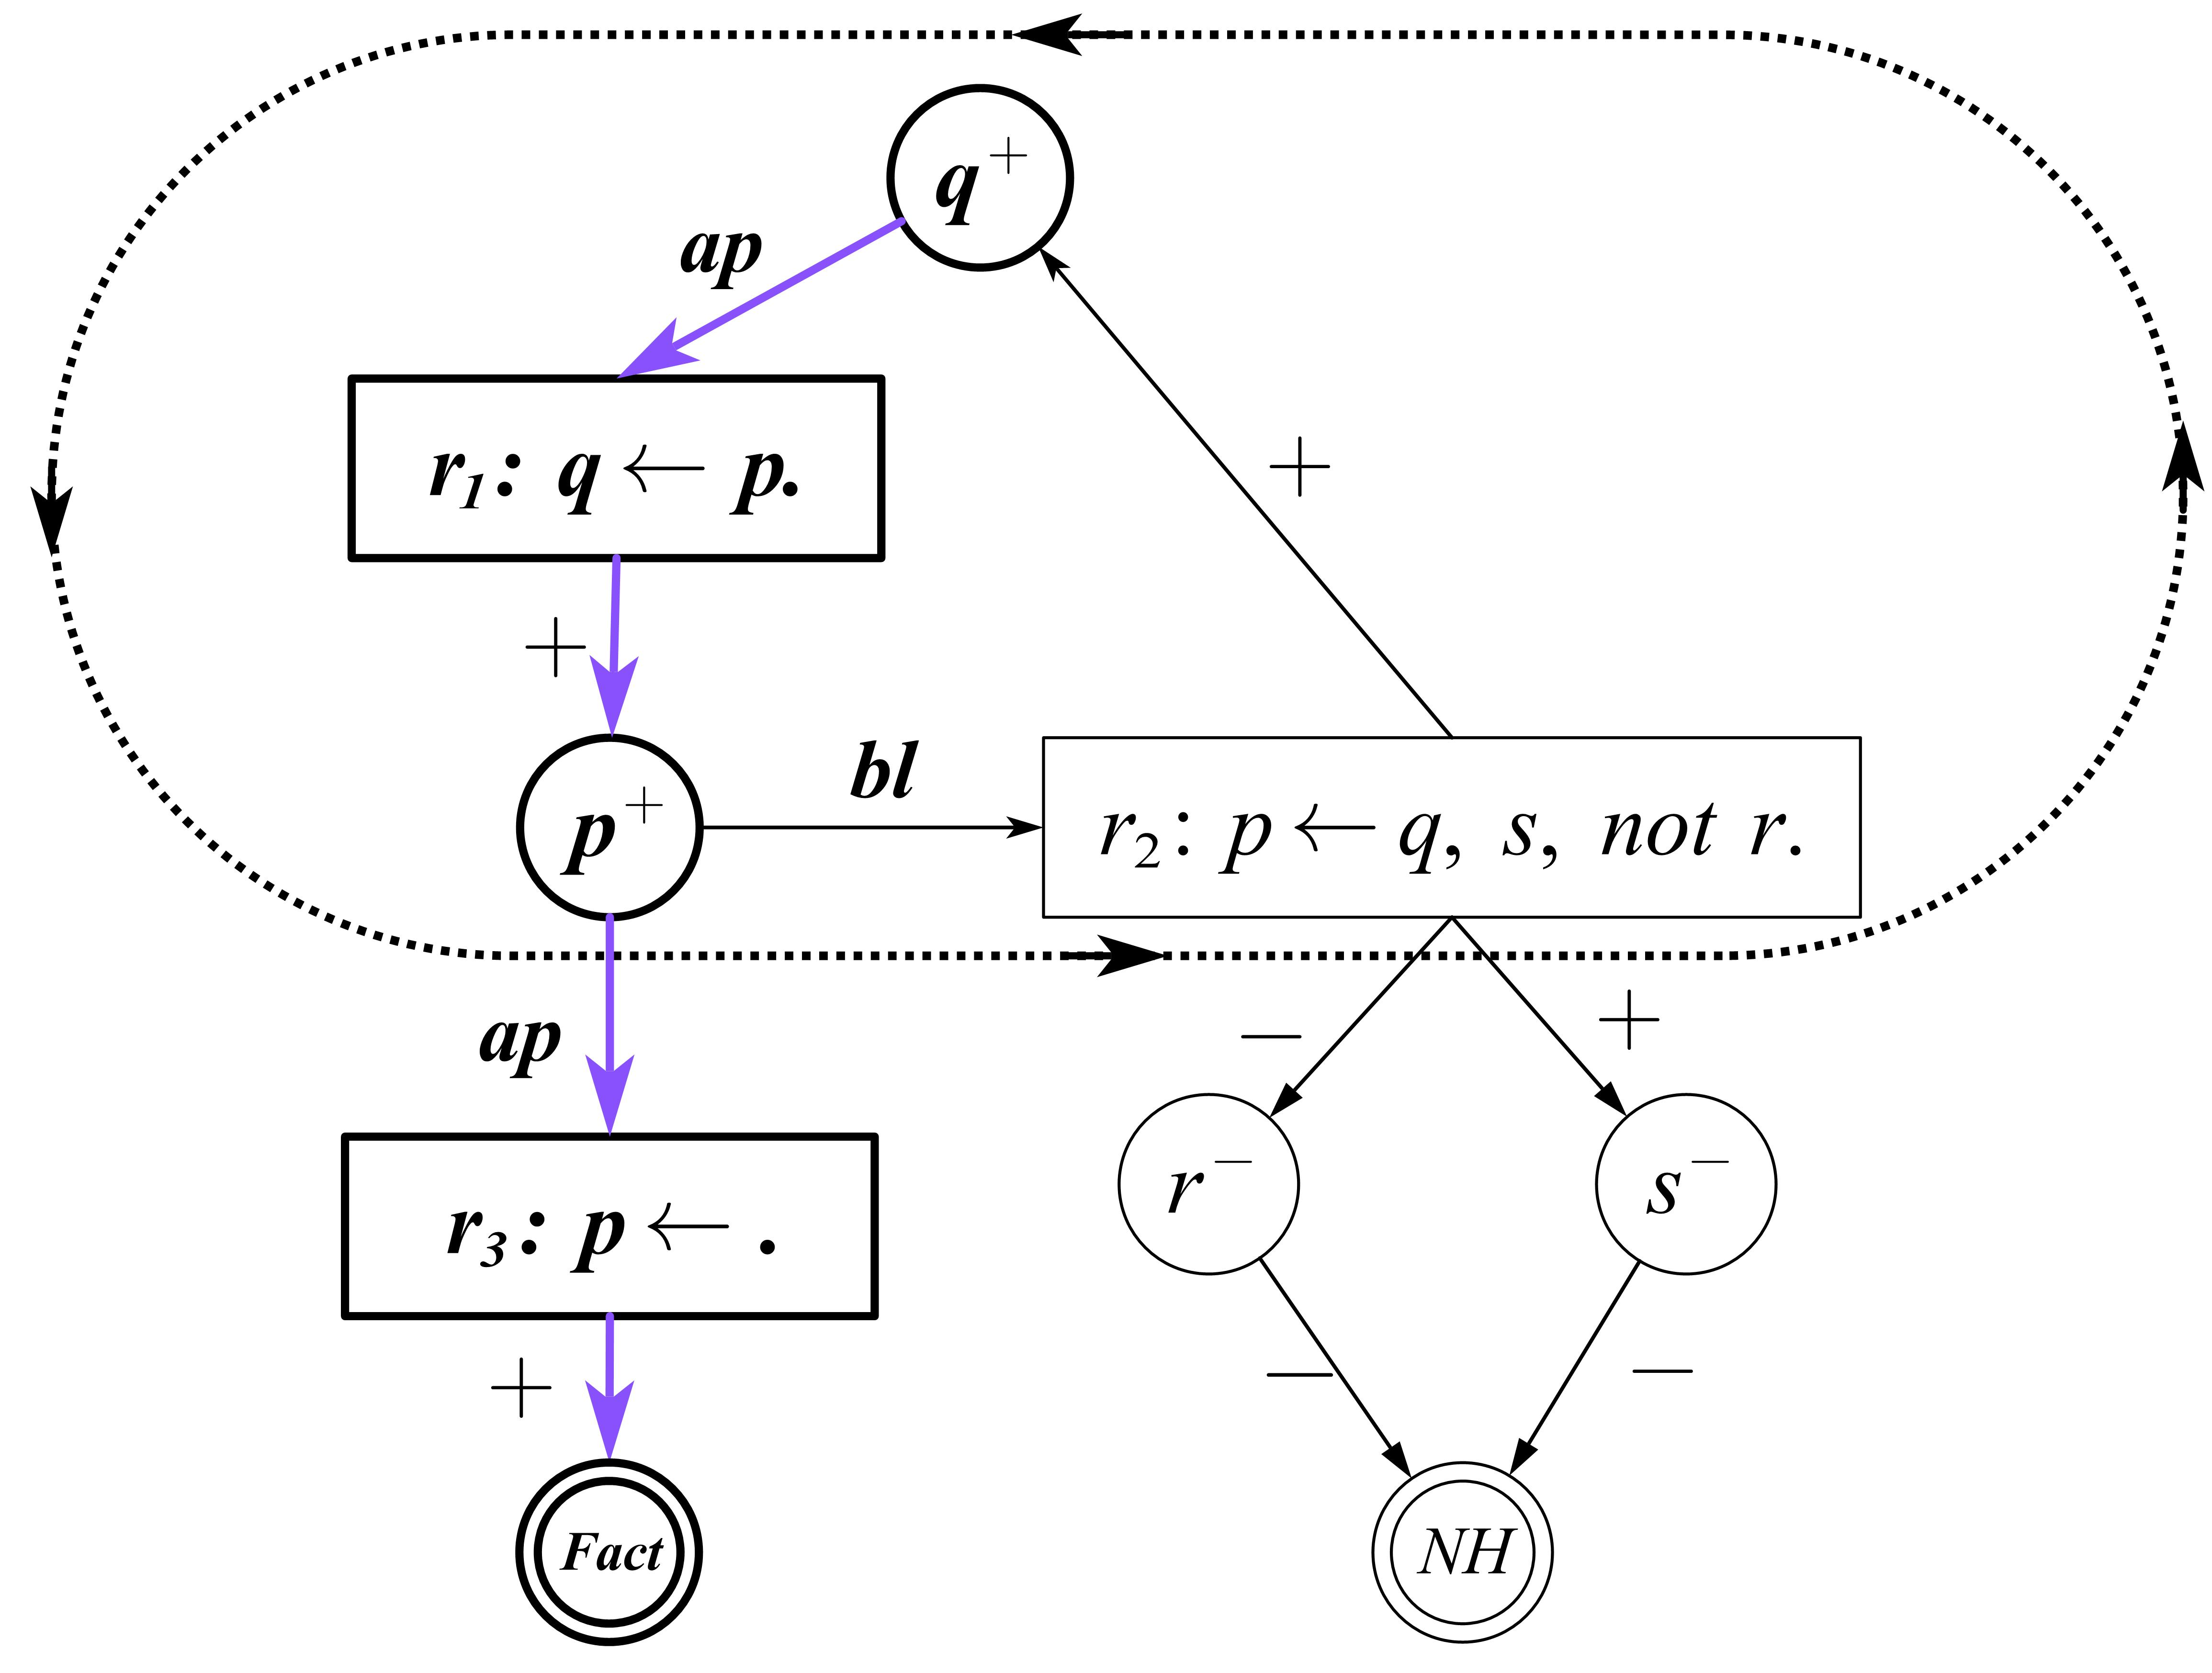
\includegraphics[height=.35\textwidth, valign=c]{figures/扩展原子规则图.jpg}} 
    \quad\quad
    \subfloat[扩展文字-规则图$ARG^{\{r\}}_{P_3}$]{\includegraphics[height=.35\textwidth, valign=c]{figures/扩展原子规则图_new.pdf}} 
    \caption{程序\hyperref[prg:p3]{$P_3$}的文字-规则图与扩展文字-规则图} 
    \label{fig:3_3} 
\end{figure}
\section{ASP扩展文字-规则图的环处理}
为了处理扩展文字-规则图中的环,首先给出扩展文字-规则图中环的形式化定义。
\begin{definition}[扩展文字-规则图中的环]
    给定一个实例化的一致性ASP程序$P$及$P$的一个回答集$M \in SM(P)$,$P$在$M$下的扩展原子图$ARG_P^M= \langle V, E \rangle$中的一条非空路径$e_1, e_2, \ldots, e_n, (e_i \in E)$对应的顶点序列为$v_1, v_2, \ldots, v_n, v_1$,其中$e_i (1 \le i \le n-1)$是从$v_i$指向$v_{i+1}$的有向边,$e_n$是从$v_n$指向$v_1$的有向边。若$\forall i \neq j \in 1 \ldots n, v_i \neq v_j$,则称该路径为$ARG_P^M$中的环,记为$cyc(P,M)$,表示为$v_1 \rightarrow v_2 \rightarrow \ldots v_{n-1} \rightarrow v_n \rightarrow v_1$。如不做特别说明,本文使用$cyc(P,M)$表示$ARG_P^M$中的一个环,必要时对一张图内不同的环使用下标加以区分。对任意的环$cyc_i(P,M)$,如果其中的所有规则依赖边均标记为“+”,称这样的环为\textbf{正环},将其记作$cyc_i^+(P,M)$,否则称为\textbf{负环},记作$cyc_i^-(P,M)$。
\end{definition}

\begin{example}[扩展文字-规则图中的环]
    如图\ref{fig:3_3}(b)所示,程序\hyperref[prg:p3]{$P_3$}关于回答集$\{r\}$的扩展文字-规则图中有两个环:负环$s^+ \rightarrow r_1 \rightarrow r^- \rightarrow r_2 \rightarrow s^+$与正环$s^+ \rightarrow r_3 \rightarrow p^+ \rightarrow r_4 \rightarrow s^+$。
\end{example}

为了避免由于环而带来的无限解释,需要为每一个环找到一个不在环中的结点相连,这样的结点称为环的\textbf{出口},其形式化定义如下:

\begin{definition}[扩展文字-规则图环出口]
    给定一个实例化一致性ASP程序$P$及$P$的一个回答集$M \in SM(P)$,$cyc(P, M)$是其扩展文字-规则图的一个环。对$v_e \in V \setminus cyc(P, M)$,若$\exists v_i \in cyc(P,M), e_i=(v_i, v_e) \in E$且$\exists v_s \in V_{sink}, v_e$可达$v_s$,则$v_e$是$cyc(P, M)$的一个出口。
\end{definition}

\begin{example}[扩展文字-规则图环出口]
    如图\ref{fig:3_3}所示,程序\hyperref[prg:p2]{$P_2$}关于回答集$\{p, q\}$的扩展文字-规则图中的正环$q^+ \rightarrow r_1 \rightarrow p^+ \rightarrow r_2 \rightarrow q^+$有一个$r_3$结点为出口,而程序\hyperref[prg:p3]{$P_3$}关于回答集$\{r\}$的负环$s^+ \rightarrow r_1 \rightarrow r^- \rightarrow r_2 \rightarrow s^+$与正环$s^+ \rightarrow r_3 \rightarrow p^+ \rightarrow r_4 \rightarrow s^+$没有出口。
\end{example}

通过对扩展文字-规则的环及环的出口的定义,可以发现没有出口的环才是导致无限解释出现的根本原因。针对这一问题,本文进一步考虑对无出口环的处理。
\subsection{无出口负环处理}
首先,考虑负环的处理。Pontelli等人在离线解释的研究中发现,对于任意一个ASP程序$P$,其回答集$M$由集合$NANT(P) \setminus (WF^+_P \cup WF^-_P)$中元素的真值唯一决定\cite{pontelli2006justifications},其中$WF^+_P$与$WF^-_P$为程序$P$的良基模型,$NANT(P)=\{b \in At \mid \exists r \in P, s.t.\ b \in body^-(r)\}$,即程序P中所有规则负体部原子构成的集合。在离线解释的研究中,Pontelli等人提出引理如下\cite{pontelli2009justifications}:
\begin{lemma}
    \label{lma:wfnonegcycle}
    给定ASP程序$P$及其一个回答集$M$,$WF_P=WF^+_P \cup WF^-_P$是其良基模型,若$a \ in WF_P$,则$a$关于$M$的离线解释(假设集合为空)中不含有负环。
\end{lemma}

基于该引理,可以得到下面的定理\ref{thm:negatomnotinwf}:%
\begin{theorem}[负环原子不在良基模型中]
    \label{thm:negatomnotinwf}
    给定ASP程序$P$及其一个回答集$M$,$WF_P=WF^+_P \cup WF^-_P$是其良基模型,对$ARG^M_P$中的任意负环$cyc^-(P, M)$,有$\forall a \in cyc^-(P, M) \cap V_{atom} \notin WF_P$。
\end{theorem}

\begin{proof}[定理\ref{thm:negatomnotinwf}的证明]
    考虑引理\ref{lma:wfnonegcycle}的逆否命题:给定ASP程序$P$及其一个回答集$M$,$WF_P=WF^+_P \cup WF^-_P$是其良基模型,若$a \in At$关于$M$的离线解释(假设集合为空)中含有负环,则$a \notin WF_P$。而$ARG^M_P$中的负环与离线解释中的负环相比,仅多出了文字结点间的显式规则结点,因此$ARG^M_P$中负环内的文字$a$一定不在良基模型中。
\end{proof}

根据定理\ref{thm:negatomnotinwf},结合负环的定义,可以将负环待处理文字的范围缩减为$NANT(P) \setminus (WF^+_P \cup WF^-_P)$中的原子。实际上,这些原子在良基语义模型构建过程中被赋值为“未定义”。当$WF^+_P \cup WF^-_P = At(P)$时,称良基模型是完全的,此时良基模型与回答集是重合的。于是考虑对程序进行修改,对不在良基模型中文字的真值作出“强制为假的假设”,使得修改后的程序具有完全的良基模型,这时程序中的各文字的解释将不会出现负环。在面向用户的解释中,为了最大程度地给用户提供交互,需要找出所有备选的假设集合,该集合满足:当通过改变程序强制使得集合中其中的文字为假时,变换后的程序具有完备的良基模型。这里提到的“强制为假”的程序变换称为负规约(negative reduct,NR),定义如下:
\begin{definition}[负规约]
    给定一个实例化的一致性一般逻辑程序$P$,$U \subseteq At$为一系列程序中原子的集合,则$P$在集合$U$下的负规约$NR(P, U)$定义为
    \begin{align}
        NR(P, U) = \{r \in P \mid head(r) \notin U\}
    \label{eq:nrpu}
    \end{align}
\end{definition}
于是程序$P$在回答集$M$下备选的假设集的集合$ASM(P,M)$定义为:
\begin{align}
    ASM(P, M) = \{U \subseteq NANT(P) \mid (U \cap M = \emptyset) \land (U \notin WF^+_P \cup WF^-_P) \land WF^+_{NR(P,U)}=M\}
\label{eq:asm}
\end{align}

式\eqref{eq:nrpu}对程序进行的负规约实际上是通过去掉程序$P$中头部在$U$中的所有规则,以使得剩余程序$NR(P, U)$无法推出$U$中文字。而式\eqref{eq:asm}试图找到同时满足如下几个条件的假设集:
\begin{itemize}[topsep=0pt]
    \setlength\itemsep{-0.3em}
    \item 集合中的所有原子来源于程序中的负体部
    \item 集合中的所有原子不在回答集中
    \item 集合中的所有原子不在良基模型中
    \item 在该集合下对程序进行负规约后,程序的良基模型与回答集重合
\end{itemize}
在这种情况下,将$ASM(P,M)$中任意一个集合中原子的不正确解释为“假定”,一方面能够打破原有解释中的负环,另一方面也还原了回答集构建过程中固有的猜测过程。下面通过程序\hyperref[prg:p_4]{$P_4$}对上述负环的处理进行说明。
\begin{example}[程序\texorpdfstring{\hyperref[prg:p_4]{$P_4$}})]
    考虑程序$P_4$:
    \begin{center}
        \begin{tabular*}{\linewidth}{rl@{\extracolsep{\fill}}ll}
        \label{prg:p_4}
          &$r_1: a \leftarrow.$ &$r_2: c \leftarrow a, not\ b.$ & $r_3: b \leftarrow not\ c.$\\ 
          &$r_4: e \leftarrow not\ d.$ &$r_5: f \leftarrow e.$ &$r_6: f \leftarrow not\ a.$
        \end{tabular*}
    \end{center}
    程序\hyperref[prg:p_4]{$P_4$}的良基模型的构建示意如图\ref{fig:3_4}所示。其良基模型最终计算为$\langle \{a,e,f\}, \{d\} \rangle$,$\{b, c\}$为“undefined”,其稳定语义模型有两个,分别为$M_1=\{a,e,f,b\}$与$M_2=\{a,e,f,c\}$。
    \begin{figure}[htbp]
        \centering 
        \includegraphics[height=.63\textwidth, valign=c]{figures/wfm计算.pdf}
        \caption{程序\hyperref[prg:p_4]{$P_4$}的良基模型计算过程示意}
        \label{fig:3_4}
    \end{figure}
    
    下面考虑该程序在两个回答集下扩展的文字-规则图$ARG^{M_1}_{P_4}$与$ARG^{M_2}_{P_4}$,如图\ref{fig:3_5}(a)与图\ref{fig:3_5}(b)所示。可以看到,在良基模型之外的$b$与$c$在稳定语义模型下通过多个回答集进行了不同的赋值,紫色路径形成的负环中包含了$b$与$c$两个原子,当$b$或$c$中任意一个原子的真值确定后,回答集也唯一确定。
    \begin{figure}[htbp]
        \centering 
        \subfloat[扩展文字-规则图$ARG_{P_4}^{\{a,e,f,c\}}$]{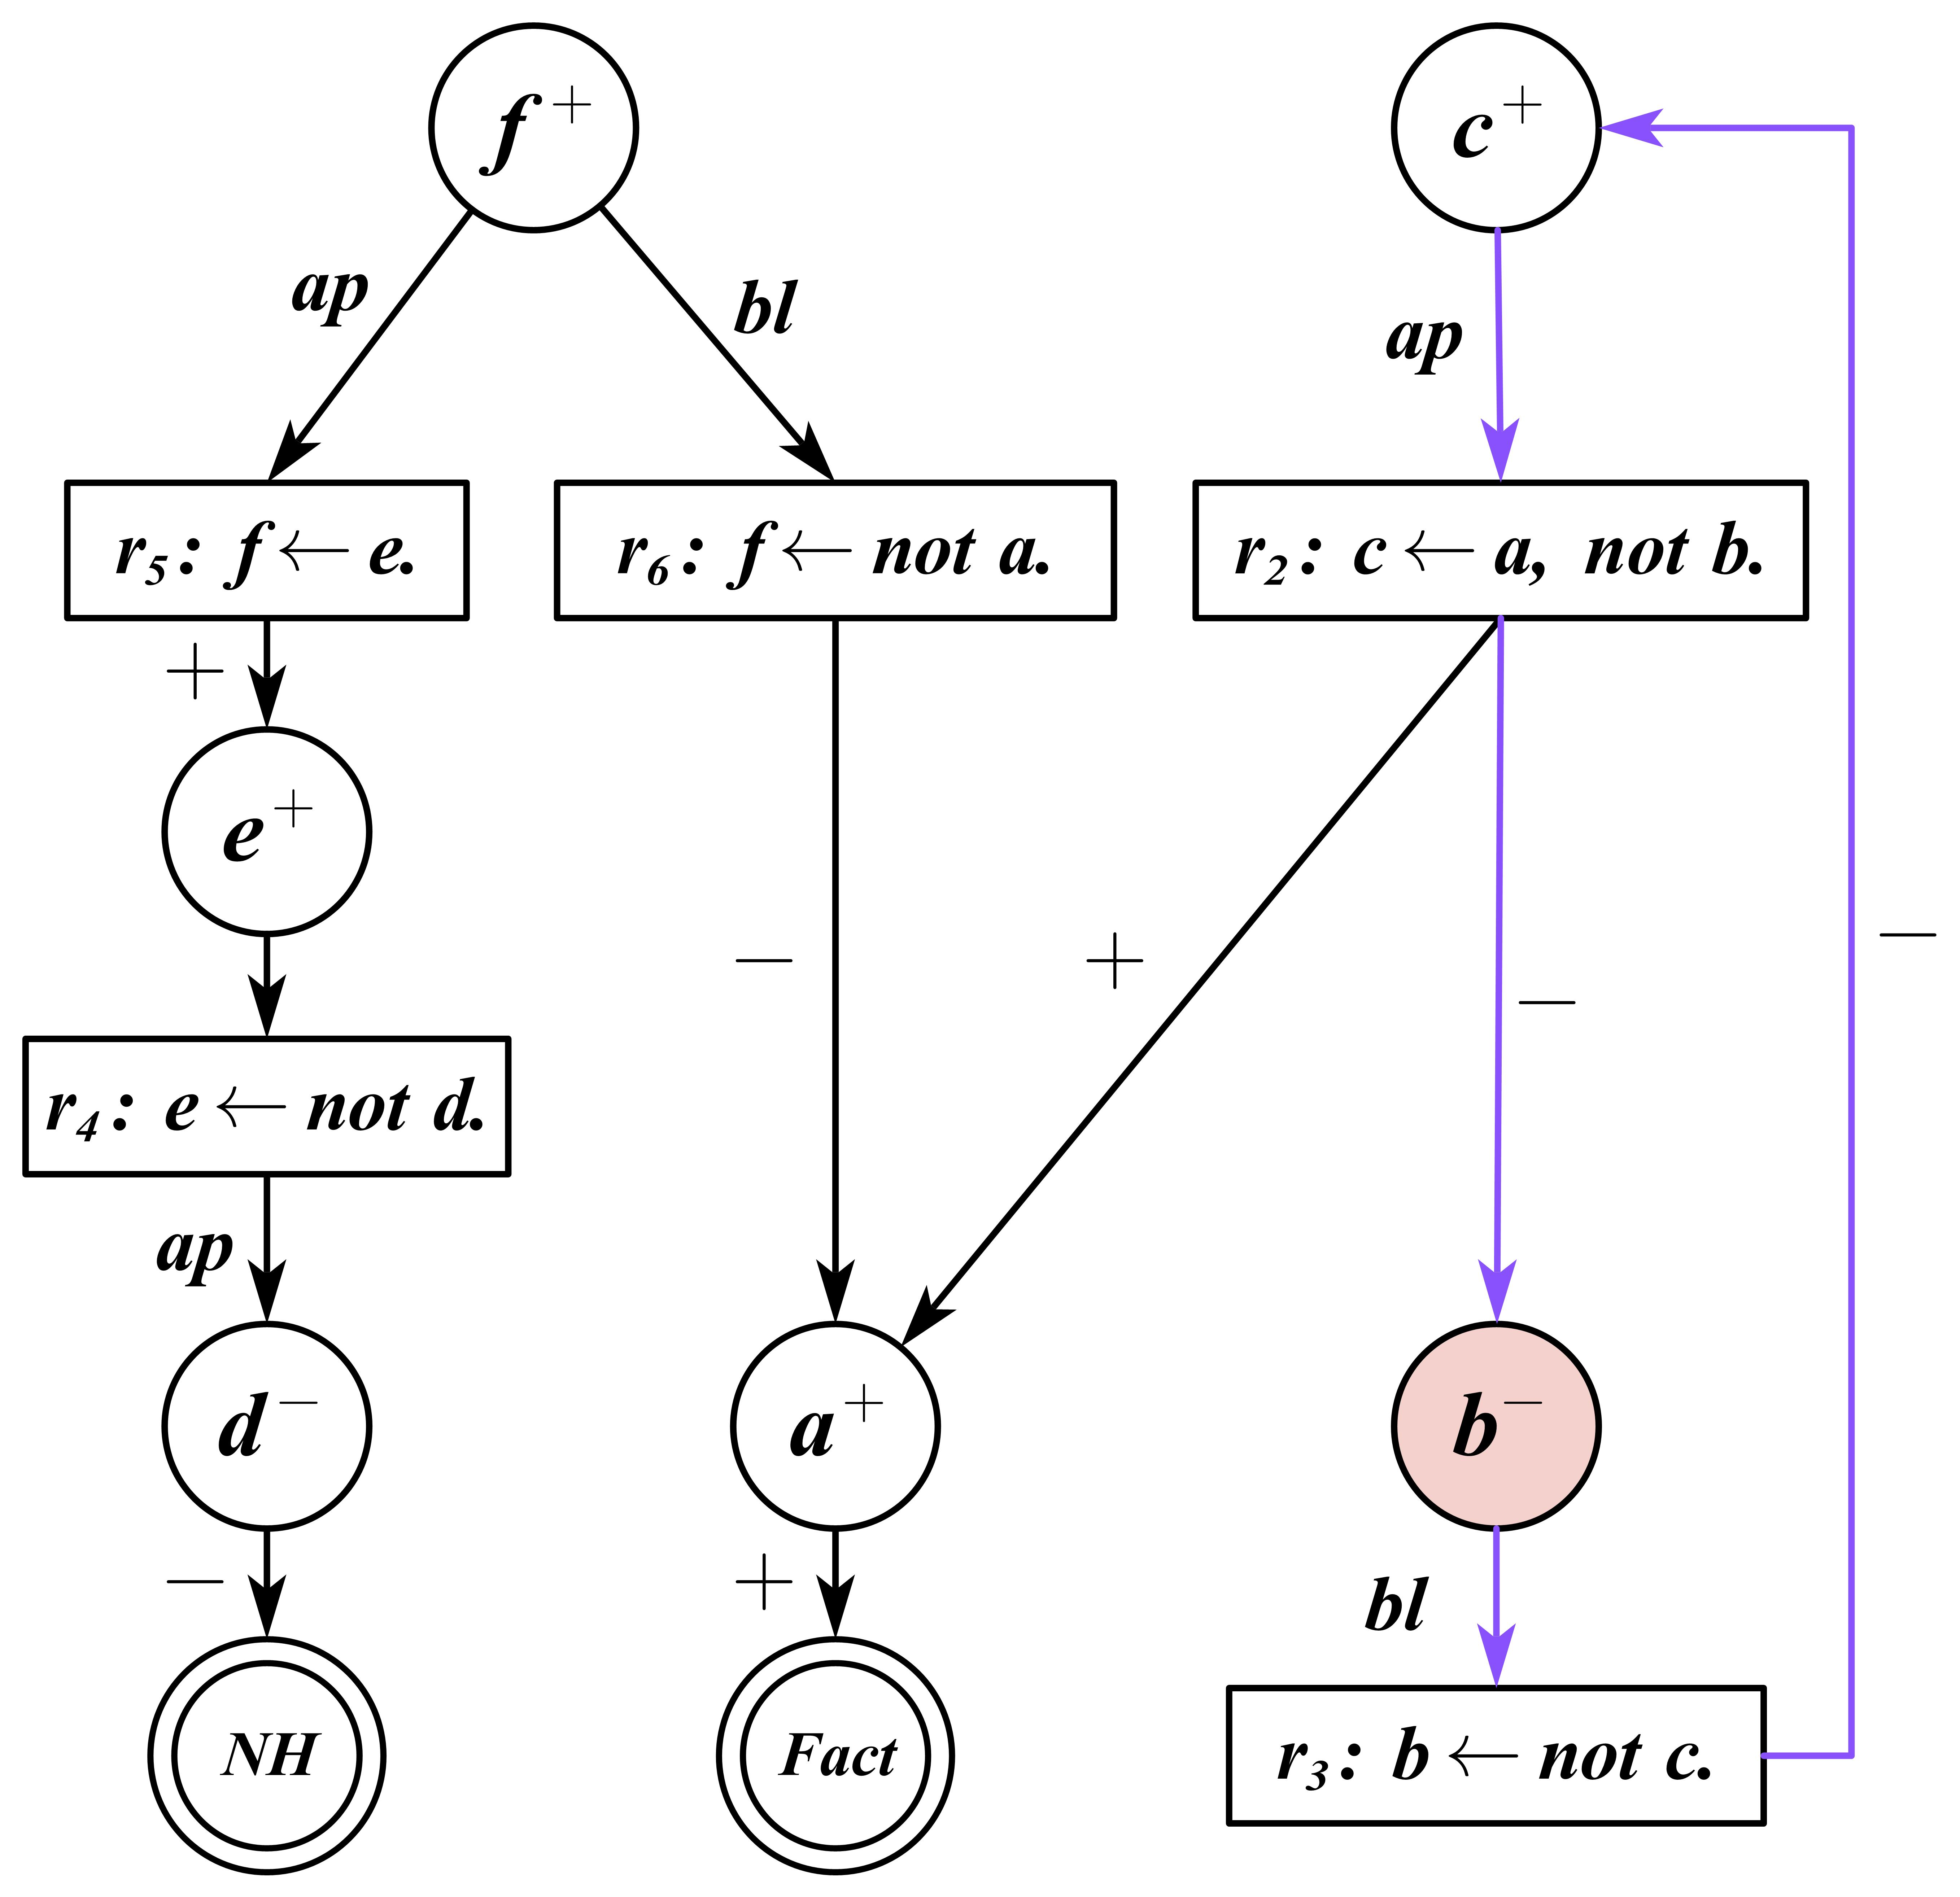
\includegraphics[height=.4\textwidth, valign=c]{figures/p4arg_m1.jpg}} 
        \quad\quad
        \subfloat[扩展文字-规则图$ARG_{P_4}^{\{a,e,f,b\}}$]{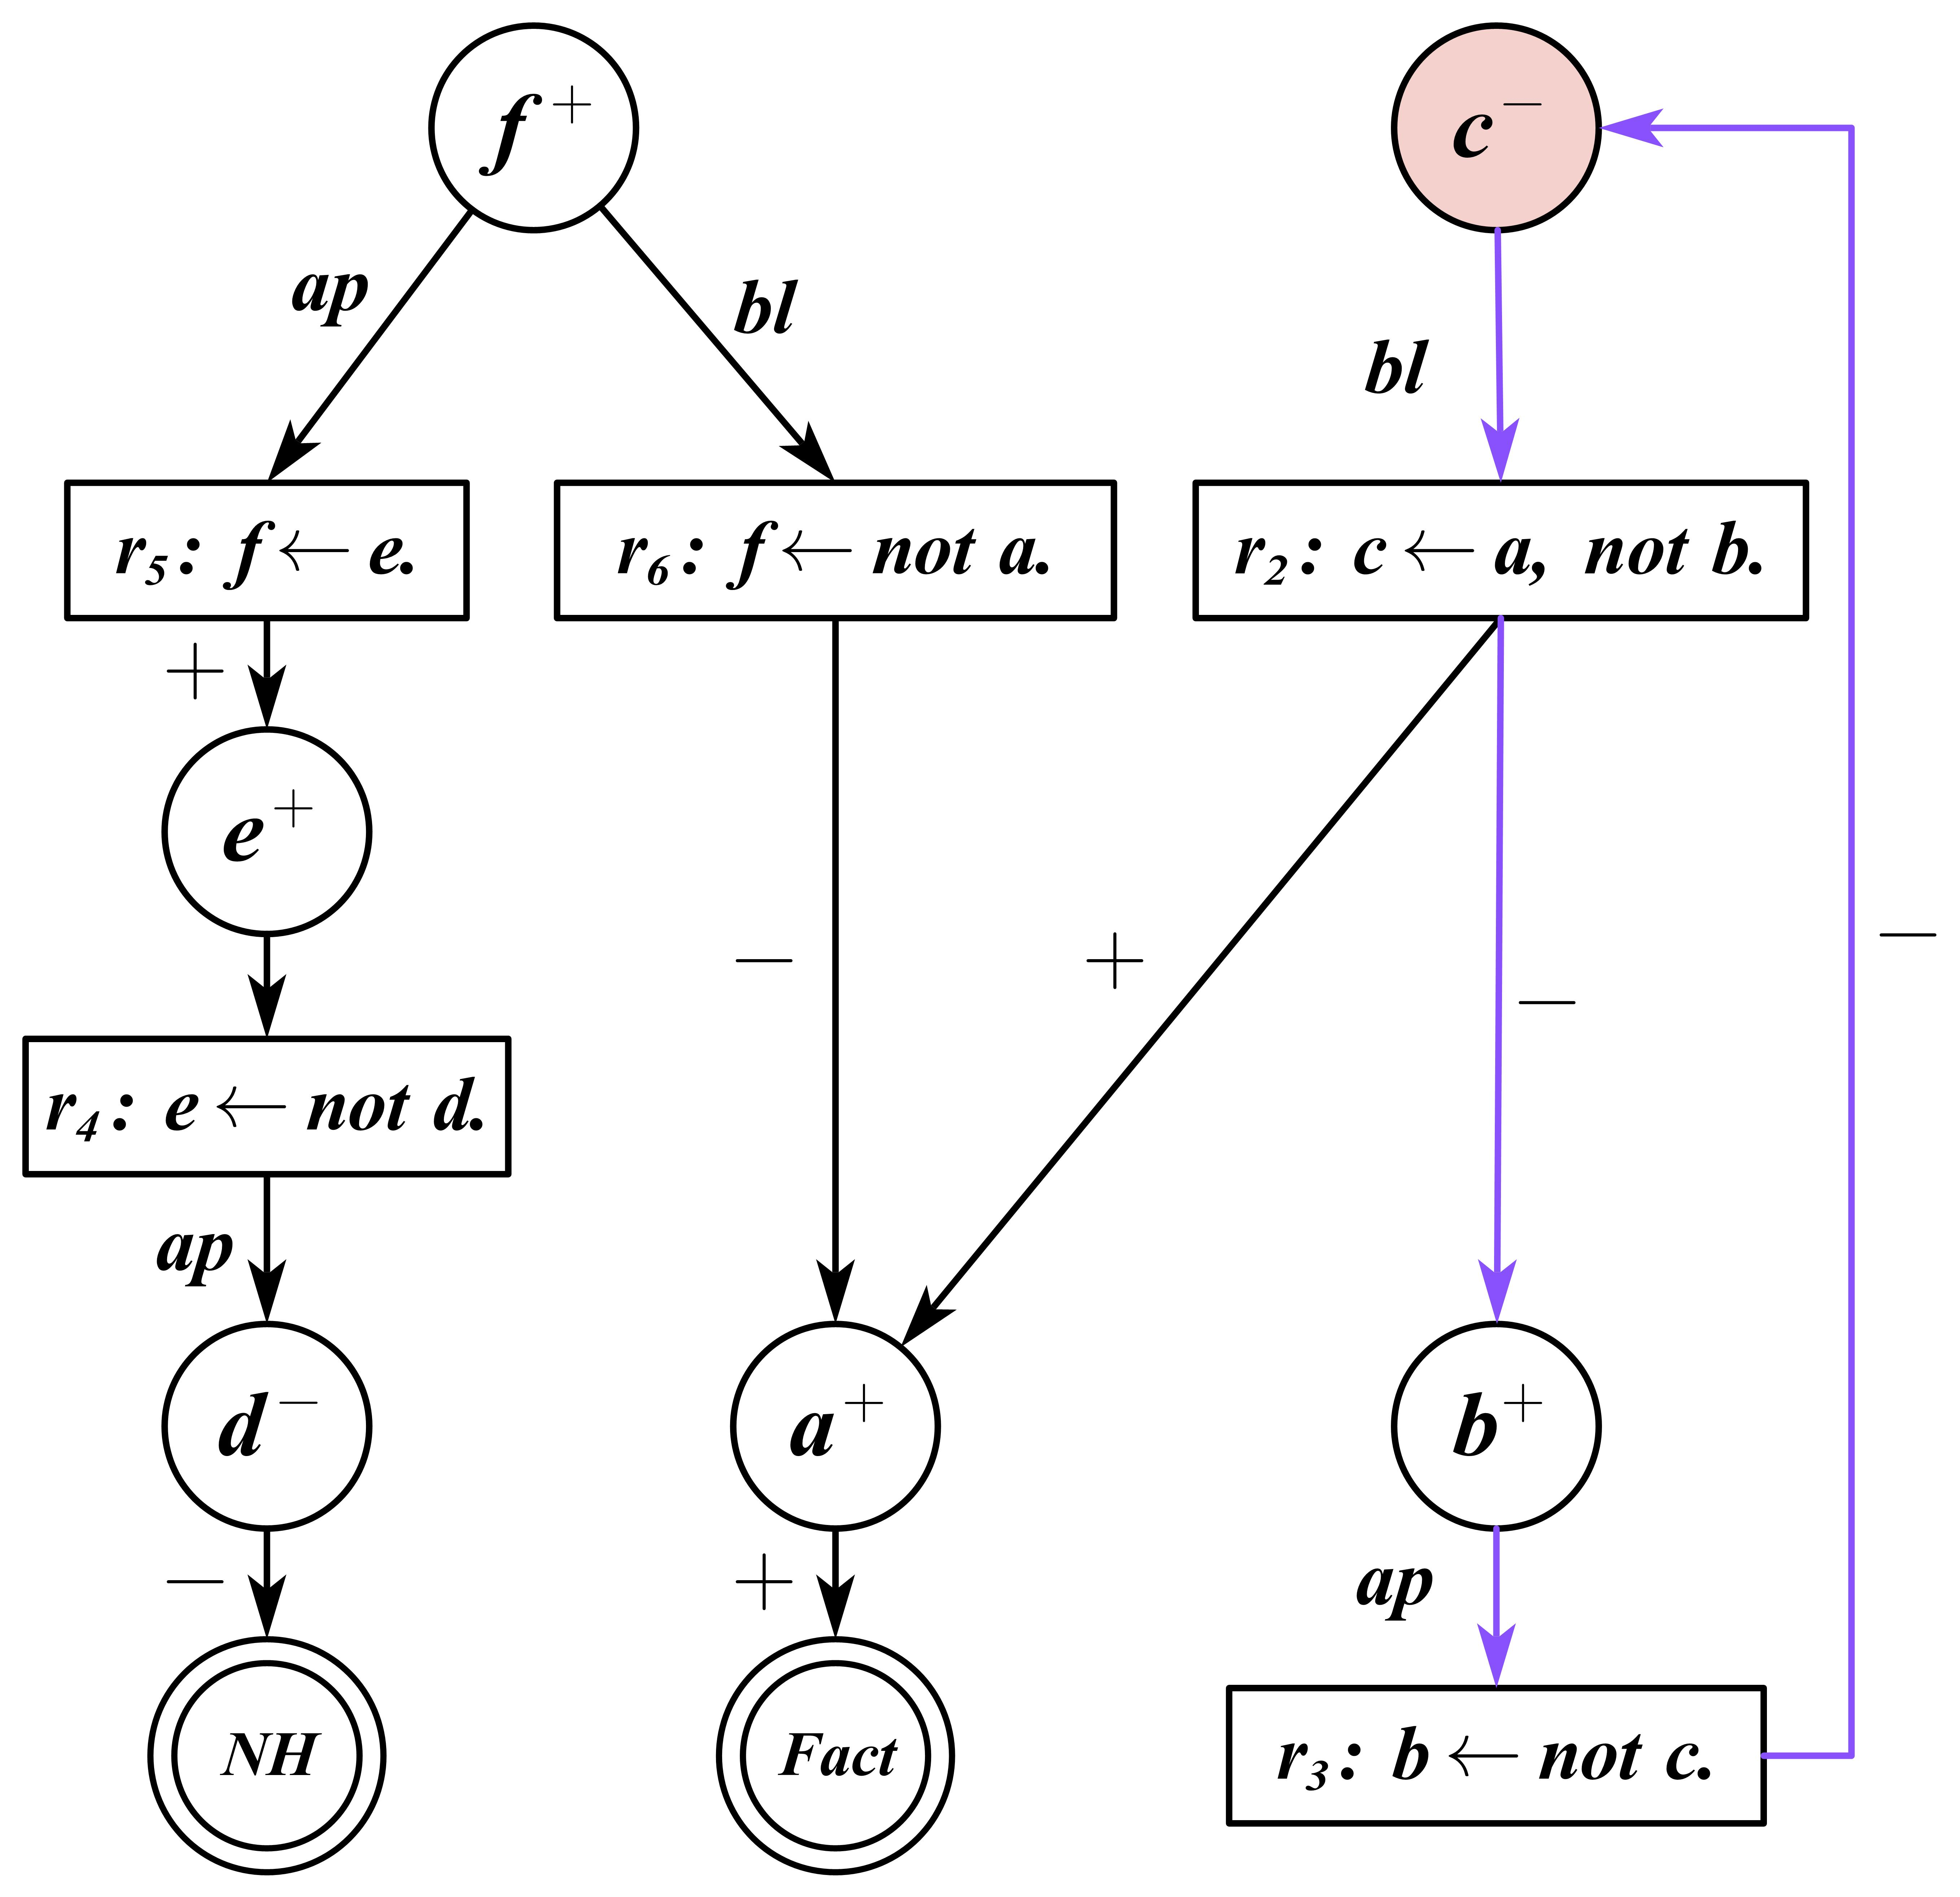
\includegraphics[height=.4\textwidth, valign=c]{figures/p4arg_m2.jpg}} 
        \caption{程序\hyperref[prg:p3]{$P_3$}的文字-规则图与扩展文字-规则图} 
        \label{fig:3_5}
    \end{figure}
    
    进一步,通过式\eqref{eq:nrpu}与\eqref{eq:asm}可以计算出备选的假设集合,其中$ASM(P_4, M_1)=\{\{b\}\}$,$ASM(P_4, M_2)=\{\{c\}\}$。
\end{example}
    需要说明的是,$ASM$集合中的元素并不一定唯一,例如程序$P_5$。
    \vspace{1ex}
    \begin{example}[程序\texorpdfstring{\hyperref[prg:p_5]{$P_5$}})]
        考虑程序$P_5$:
        \begin{center}
            \begin{tabular*}{\linewidth}{rl@{\extracolsep{\fill}}ll}
            \label{prg:p_5}
              &$r_1: p \leftarrow not\ q.$ &$r_2: q \leftarrow not\ p.$\\ 
              &$r_3: r \leftarrow not\ p.$ &$r_4: s \leftarrow not\ r.$
            \end{tabular*}
        \end{center}
        程序\hyperref[prg:p_5]{$P_5$}的良基模型计算为$\langle \emptyset, \emptyset \rangle$,所有文字均为“undefined”,其稳定语义模型有两个,分别为$M_1=\{p,s\}$与$M_2=\{q,r\}$。通过计算可以得到$ASM(P_5, M_1)=\{\{q\}, \{q, r\}\}\}$。图\ref{fig:3_6}给出了$ARG^{M_1}_{P_5}$及其环示意。此时,将$\{q\}$或$\{q,r\}$不在回答集中解释为假设为假,均能够避免在解释中出现环。
        \begin{figure}[!h]
            \centering 
            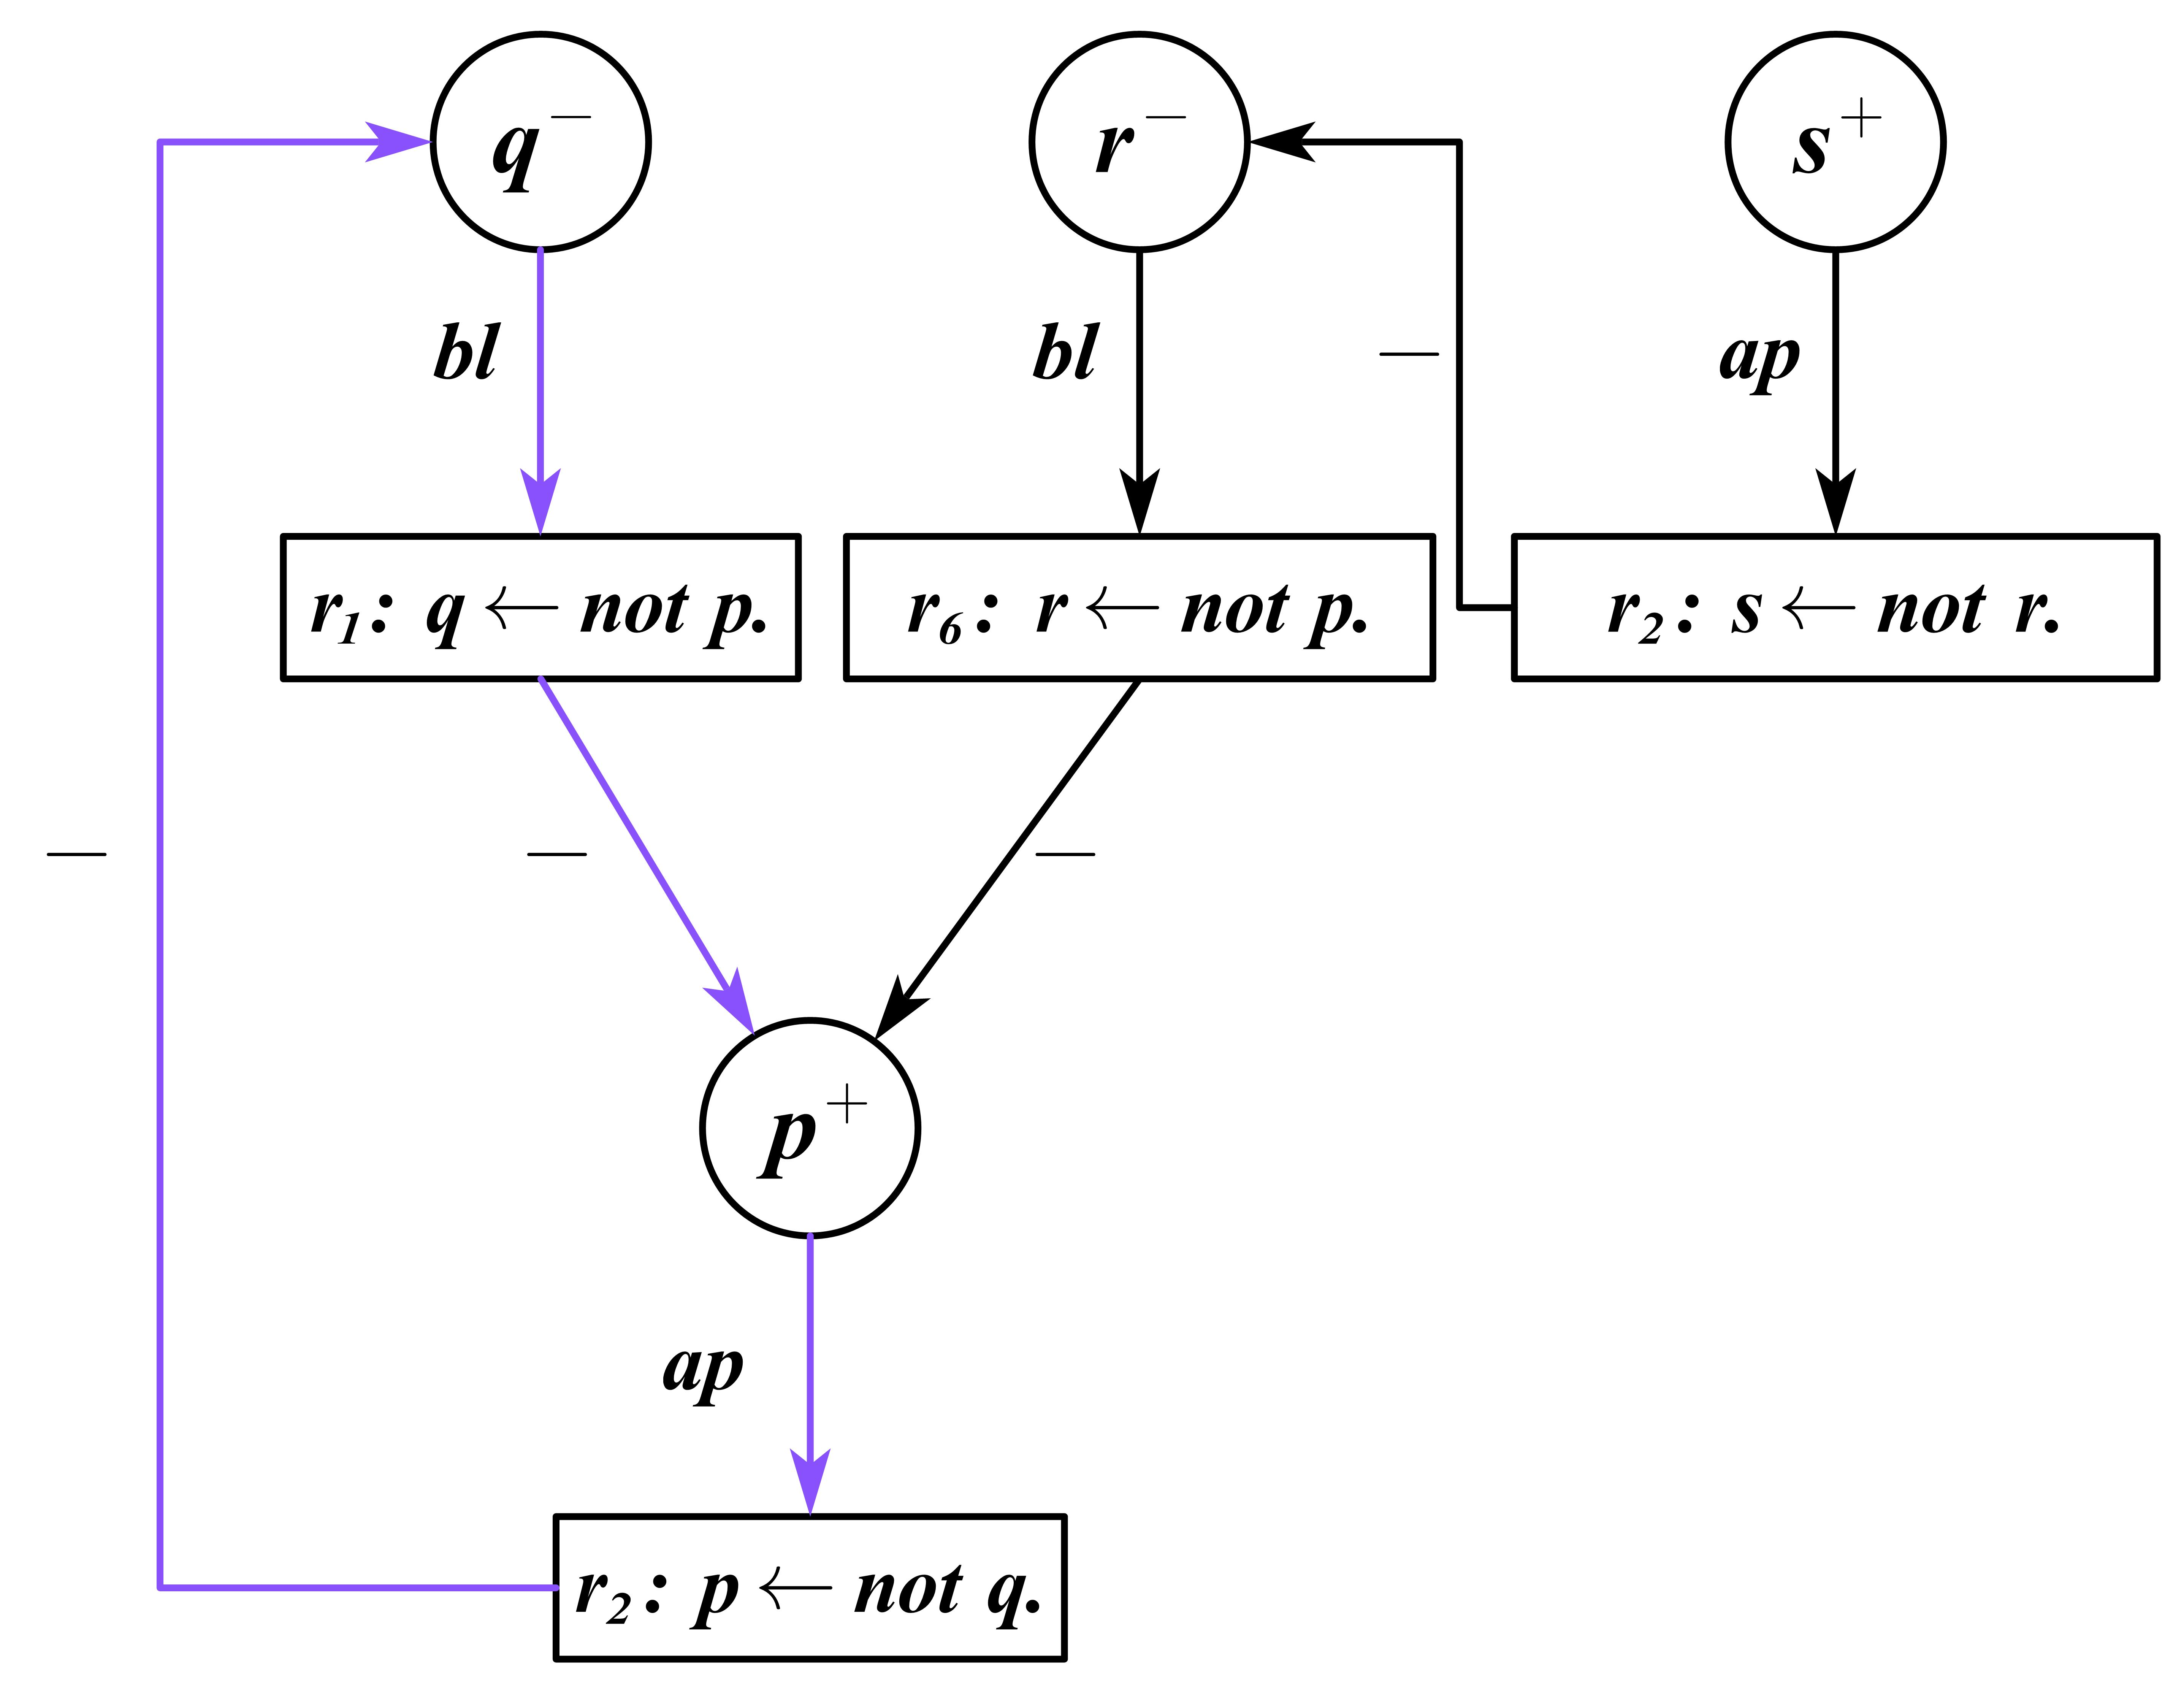
\includegraphics[height=.4\textwidth, valign=c]{figures/argp5m1.jpg}
            \caption{程序\hyperref[prg:p_5]{$P_5$}的扩展文字-规则图$ARG^{M_1}_{P_5}$}
            \label{fig:3_6}
        \end{figure}
    \end{example}
    事实上,上述研究展现了程序中负环的出现,是由于某些原子真值的不确定性。在二值逻辑下的稳定语义模型中,每个原子的真值或为真或为假,因此得到回答集的过程是一种固有的“猜测-验证”(Guess and Check)的过程\cite{eiterASP2009}。而通过上述$ASM$集合的定义,为找到这些原子提供了一种形式化的计算方法,同时也能够将集合中的原子为假归因于这一假设,从而不再由于负环中原子间的相互依赖而产生循环解释。
\subsection{无出口正环处理}
    解决了负环处理的问题后,本文接着对扩展文字-规则图中的正环特性进行研究。对无出口正环的分析基于Lin与Zhao等人提出的逻辑程序环公式\cite{lin2004assat},将其定义推广到扩展文字-规则图下。

\begin{definition}[正环的外部支持]
    给定一个实例化一致性ASP程序$P$及$P$的一个回答集$M \in SM(P)$,对$ARG^M_P$中任意的正环$cyc^+(P, M)$,记$ES_P(cyc^+(P, M))$为$cyc^+(P, M)$在程序$P$与回答集$M$下的外部支持,$EB_P(cyc^+(P, M))$为$cyc^+(P, M)$在程序$P$与回答集$M$下的外部体部集,定义如下:
    \begin{align}
        &\mathit{ES_P(cyc^+(P, M)) = \{ r \in P \mid head(r) \in cyc^+(P, M), body^+(r) \cap cyc^+(P, M) = \emptyset\}}\\
        &\mathit{EB_P(cyc^+(P, M)) = \{body(r) \mid r \in ES_P(cyc^+(P, M)) \}}
      \end{align}
\end{definition}
\begin{example}
    程序\hyperref[prg:p3]{$P_3$}在回答集$\{s, p\}$下的正环$cyc^+(P_3, \{r\})=s^+ \rightarrow r_3 \rightarrow p^+ \rightarrow r_4 \rightarrow s^+$的外部支持$ES_P(cyc^+(P_3, \{r\}))=\{r_1\}$,外部体部集为$EB_P(cyc^+(P_3, \{r\}))=\{not\ r\}$,由于$\{not\ r\}$成立,该环得到了外部支持,环内个文字均成立;而其在另一个回答集$\{r\}$下的正环$cyc+(P_3, \{r\})=s^- \rightarrow r_1 \rightarrow p^- \rightarrow r_4 \rightarrow s^-$的外部支持与$cyc^+(P_3, \{r\})$相同,但由于在该回答集下,$\{not\ r\}$不成立,该环没有得到外部支持,因此$s$与$r$在该回答集下均不成立。
\end{example}

显然,当正环的至少一条外部支持规则适用时,规则头部成立,正环内的文字得到支持;如果所有的外部支持规则都不适用,则正环内的文字无法得到支持,环内所有文字均不成立。这一结论被形式化地定义为环公式:

\begin{definition}[正环的环公式]
    给定一个ASP程序$P$及$P$的一个回答集$M \in SM(P)$,$r\in P$是其中的一条规则,定义$BF(body(r))$为规则$r$正体部与负体部文字的合取,即
    \begin{align}
        BF(body(r))=\bigwedge_{l \in body^+(r)} l \land \bigwedge_{l \in body^-(r)} \lnot l
      \end{align}
    正环$cyc^+(P, M)$的环公式定义为:
    \begin{align}
        \begin{split}
            \mathit{LF_P(cyc^+(P, M))} &\mathit{= \left( \bigvee_{l \in cyc^+(P, M)} l \right)  \rightarrow \left(\bigvee_{body(r)\in EB_P(cyc^+(P, M))}BF(body(r))\right)}\\ 
        &\mathit{\equiv  \left(\bigwedge_{body(r) \in EB_P(cyc^+(P, M))} \lnot BF(body(r)) \right) \rightarrow  \left( \bigwedge_{l \in cyc^+(P, M)} \lnot l \right)} \label{eq:loopformula}
        \end{split}
        \end{align}
\end{definition}

式\eqref{eq:loopformula}中可以看到,对于任意一个正环而言,如果环外的规则都不能被适用,那么环内所有文字均不正确。Pontelli等人在离线解释研究中的发现,离线解释图中的环(负环已通过$ASM$集合假设进行处理),只可能是结点各文字均为假且相互依赖的环\cite{pontelli2009justifications},这一结论与本文的发现相一致,这里从环公式的视角再次印证了这一结论。因此,本文将这一性质作为正环内文字均为假的原因并在解释中呈现。

\section{ASP程序解释空间及其构建算法设计}
\subsection{ASP程序解释空间定义}
在处理完程序中的没有出口的正环与负环后,本文对扩展文字-规则图$ARG$进一步改进,提出ASP程序的解释空间(Explanation Universe,EU),具体定义如下:
\begin{definition}[ASP程序解释空间]
    给定一个一致的ASP程序$P$及其一个回答集$M \in SM(P)$,程序$P$在$M$下的解释空间基于$ARG^P_M$定义,在其基础上作出如下修改:
    \begin{itemize}[topsep=0pt]
        \setlength\itemsep{-0.3em}
        \item $V_{sink} = V_{sink} \cup \{ASM\} \cup \{UE\}$,即扩充定义两个新类型的汇结点,其中$ASM$表示“假设为假”,$UE$表示未得到外部支持;
        \item $E_{end} = E_{end} \cup E_{ue} \cup E_{asm}$,即在终结边的基础上增加两种新的边:
        \begin{itemize}[topsep=0pt,label=$\circ$]
            \setlength\itemsep{-0.3em}
            \item $E_{ue} = \{(v, -, UE) \mid v \in cyc^+(P, M), cyc^+(P, M)\text{ 未受到外部支持}\}$
            \item $E_{end} = \{(v, -, ASM) \mid v \in cyc^-(P, M), \exists U \in ASM(P, M), v \in U\}$
        \end{itemize}
    \end{itemize}
\end{definition}

\begin{example}[程序\texorpdfstring{\hyperref[prg:p_4]{$P_4$}})]
    程序$P_4$的两个回答集分别是$M_1=\{p,s\}$与$M_2=\{r\}$。在$\{p,s\}$下计算得到的备选假设集为$\{\{r\}\}$,而在$\{r\}$下计算得到的备选假设集为$\{\{s\}, \{p,s\}\}$。图\ref{fig:3_7}(a)中,橘黄色路径构成一个未被外部支持的正环,因此$s^-$与$p^-$均与$UE$结点相连,同时该解释空间对$\{s\}$为假作出基于假设的解释,因此$s^-$与$ASM$结点相连;图\ref{fig:3_7}(b)中,橘黄色路径构成的正环得到了外部规则$r_1$的支持,因此$s^-$与$p^-$均与$UE$结点相连,同时该解释空间对$\{r\}$为假作出基于假设的解释,因此$r^-$与$ASM$结点相连。
    \begin{figure}[htbp]
        \centering 
        \subfloat[程序$P_4$的解释空间$EU^{P_4}_{\{r\}, \{s\}}$]{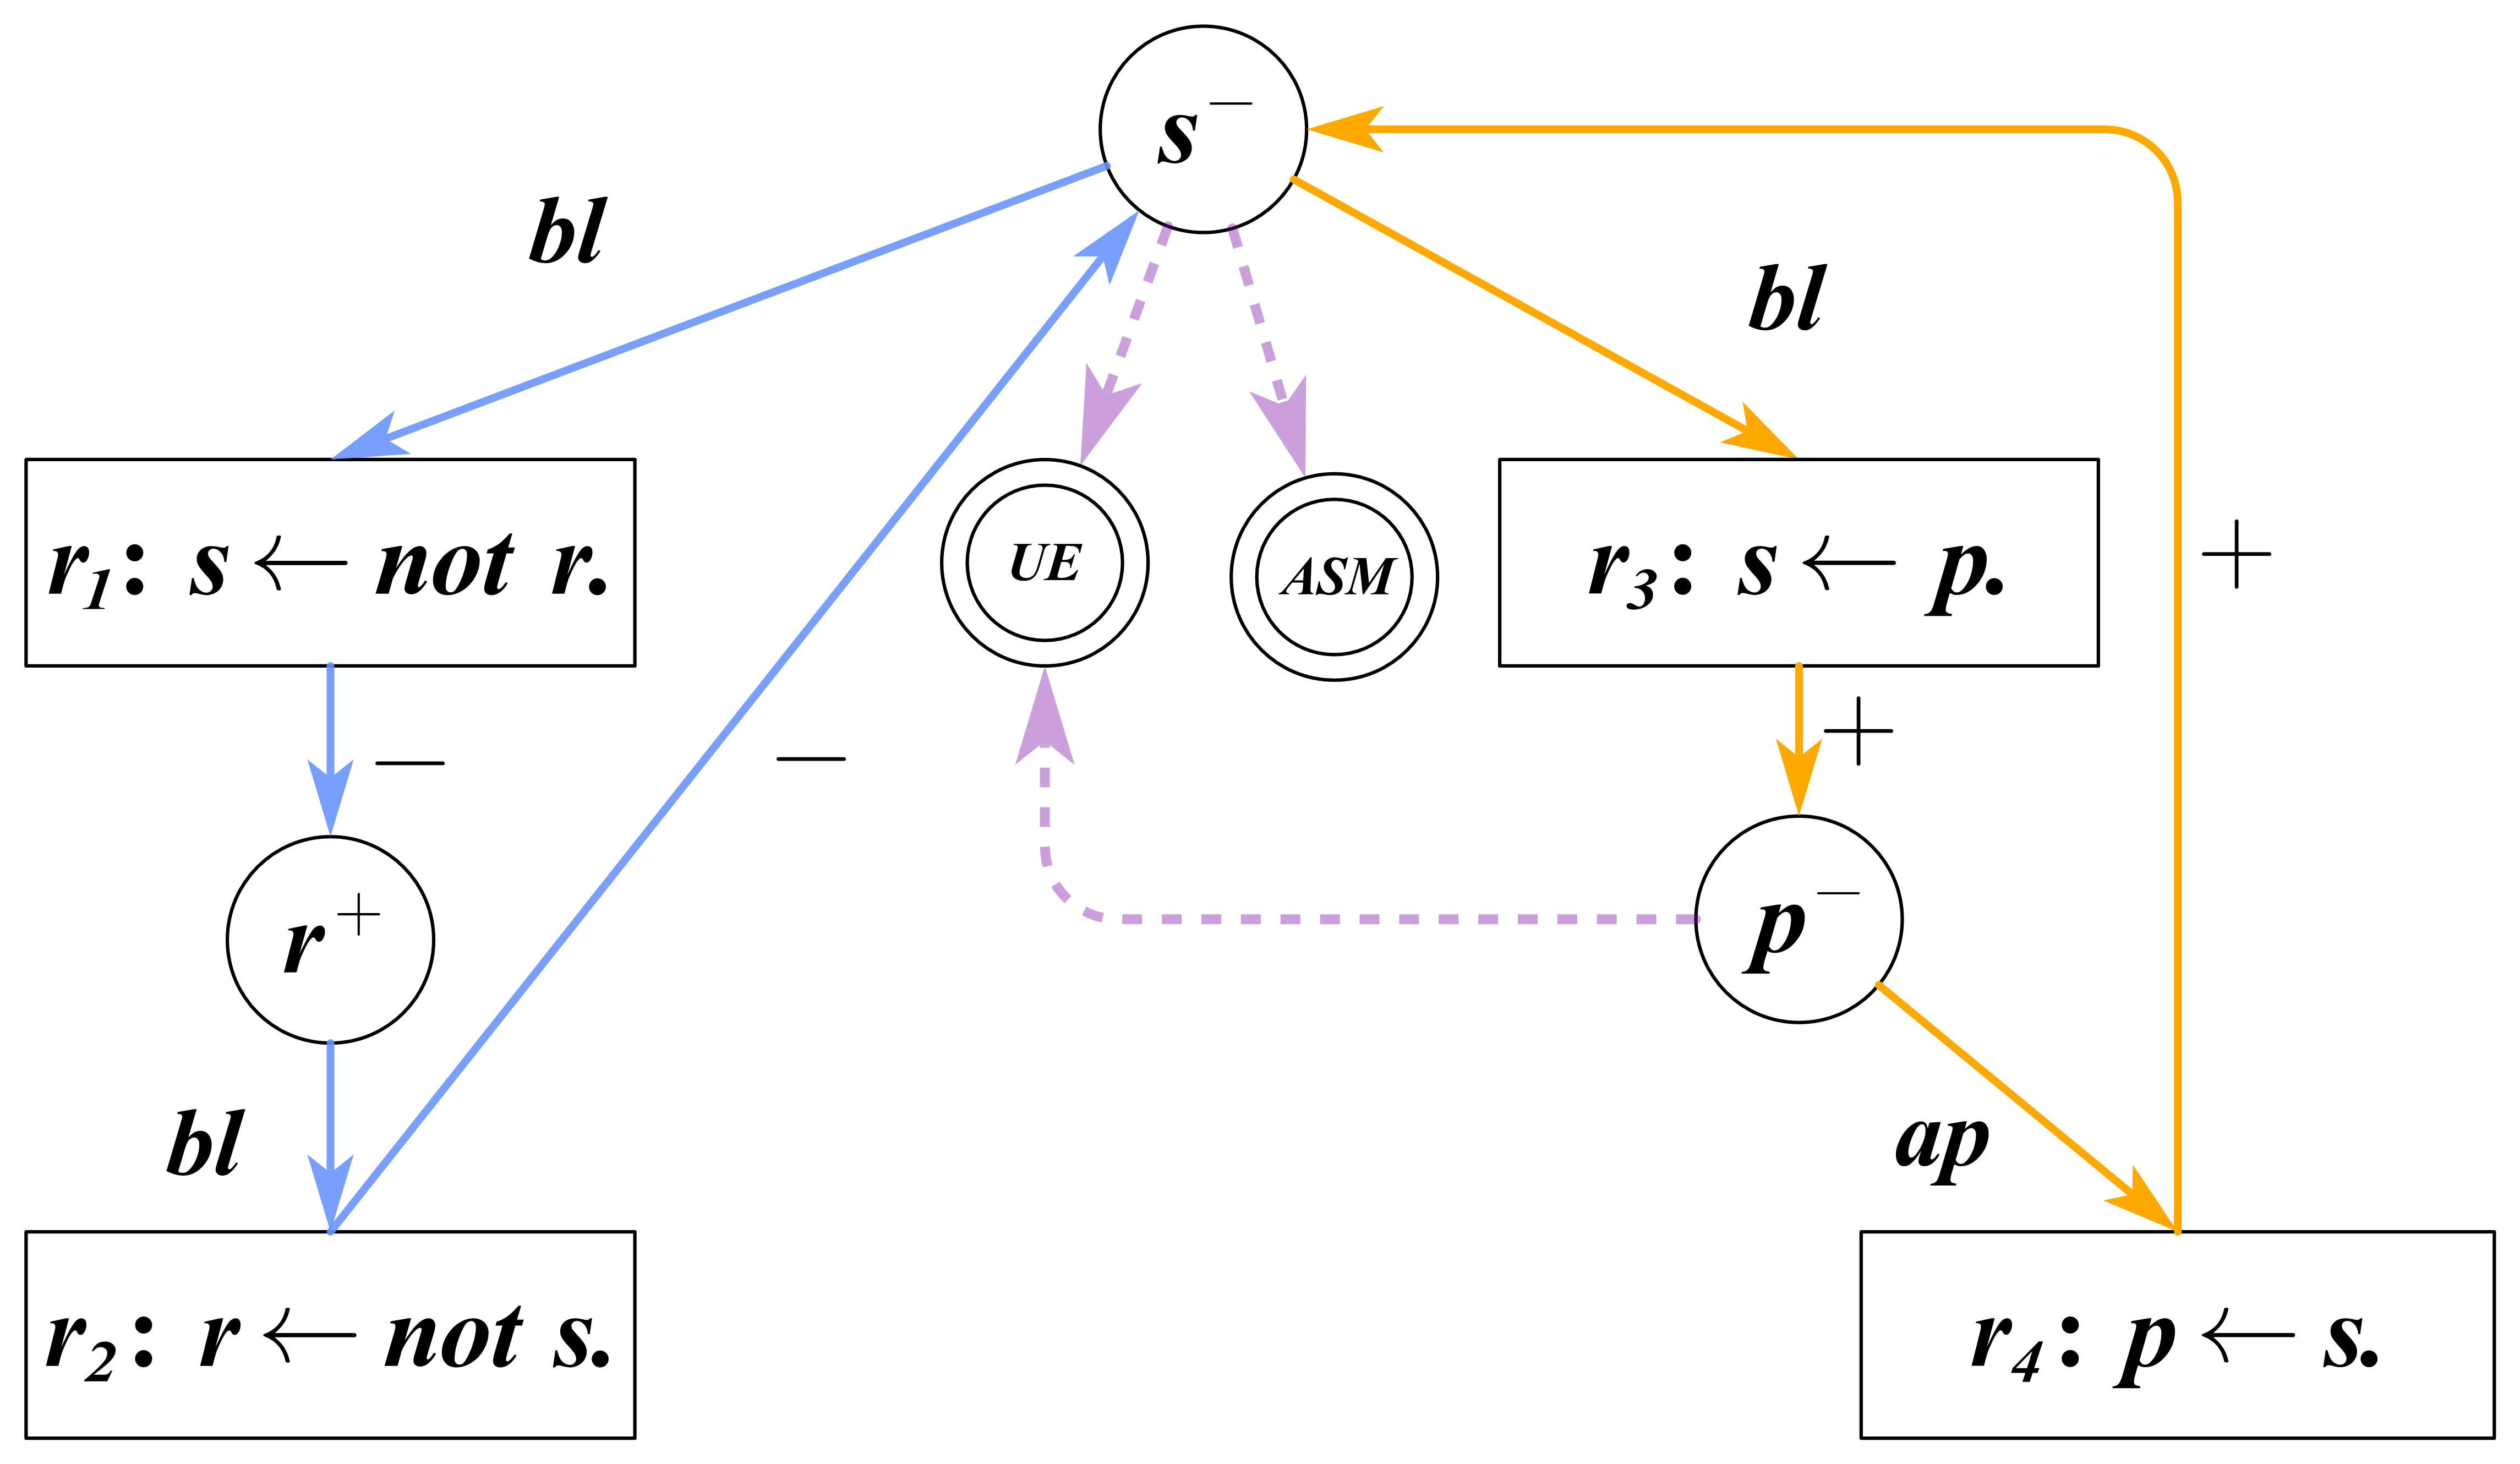
\includegraphics[height=.25\textwidth, valign=c]{figures/解释空间_1.jpg}} 
        \quad\quad
        \subfloat[程序$P_4$的解释空间$EU^{P_4}_{\{p, s\}, \{r\}}$]{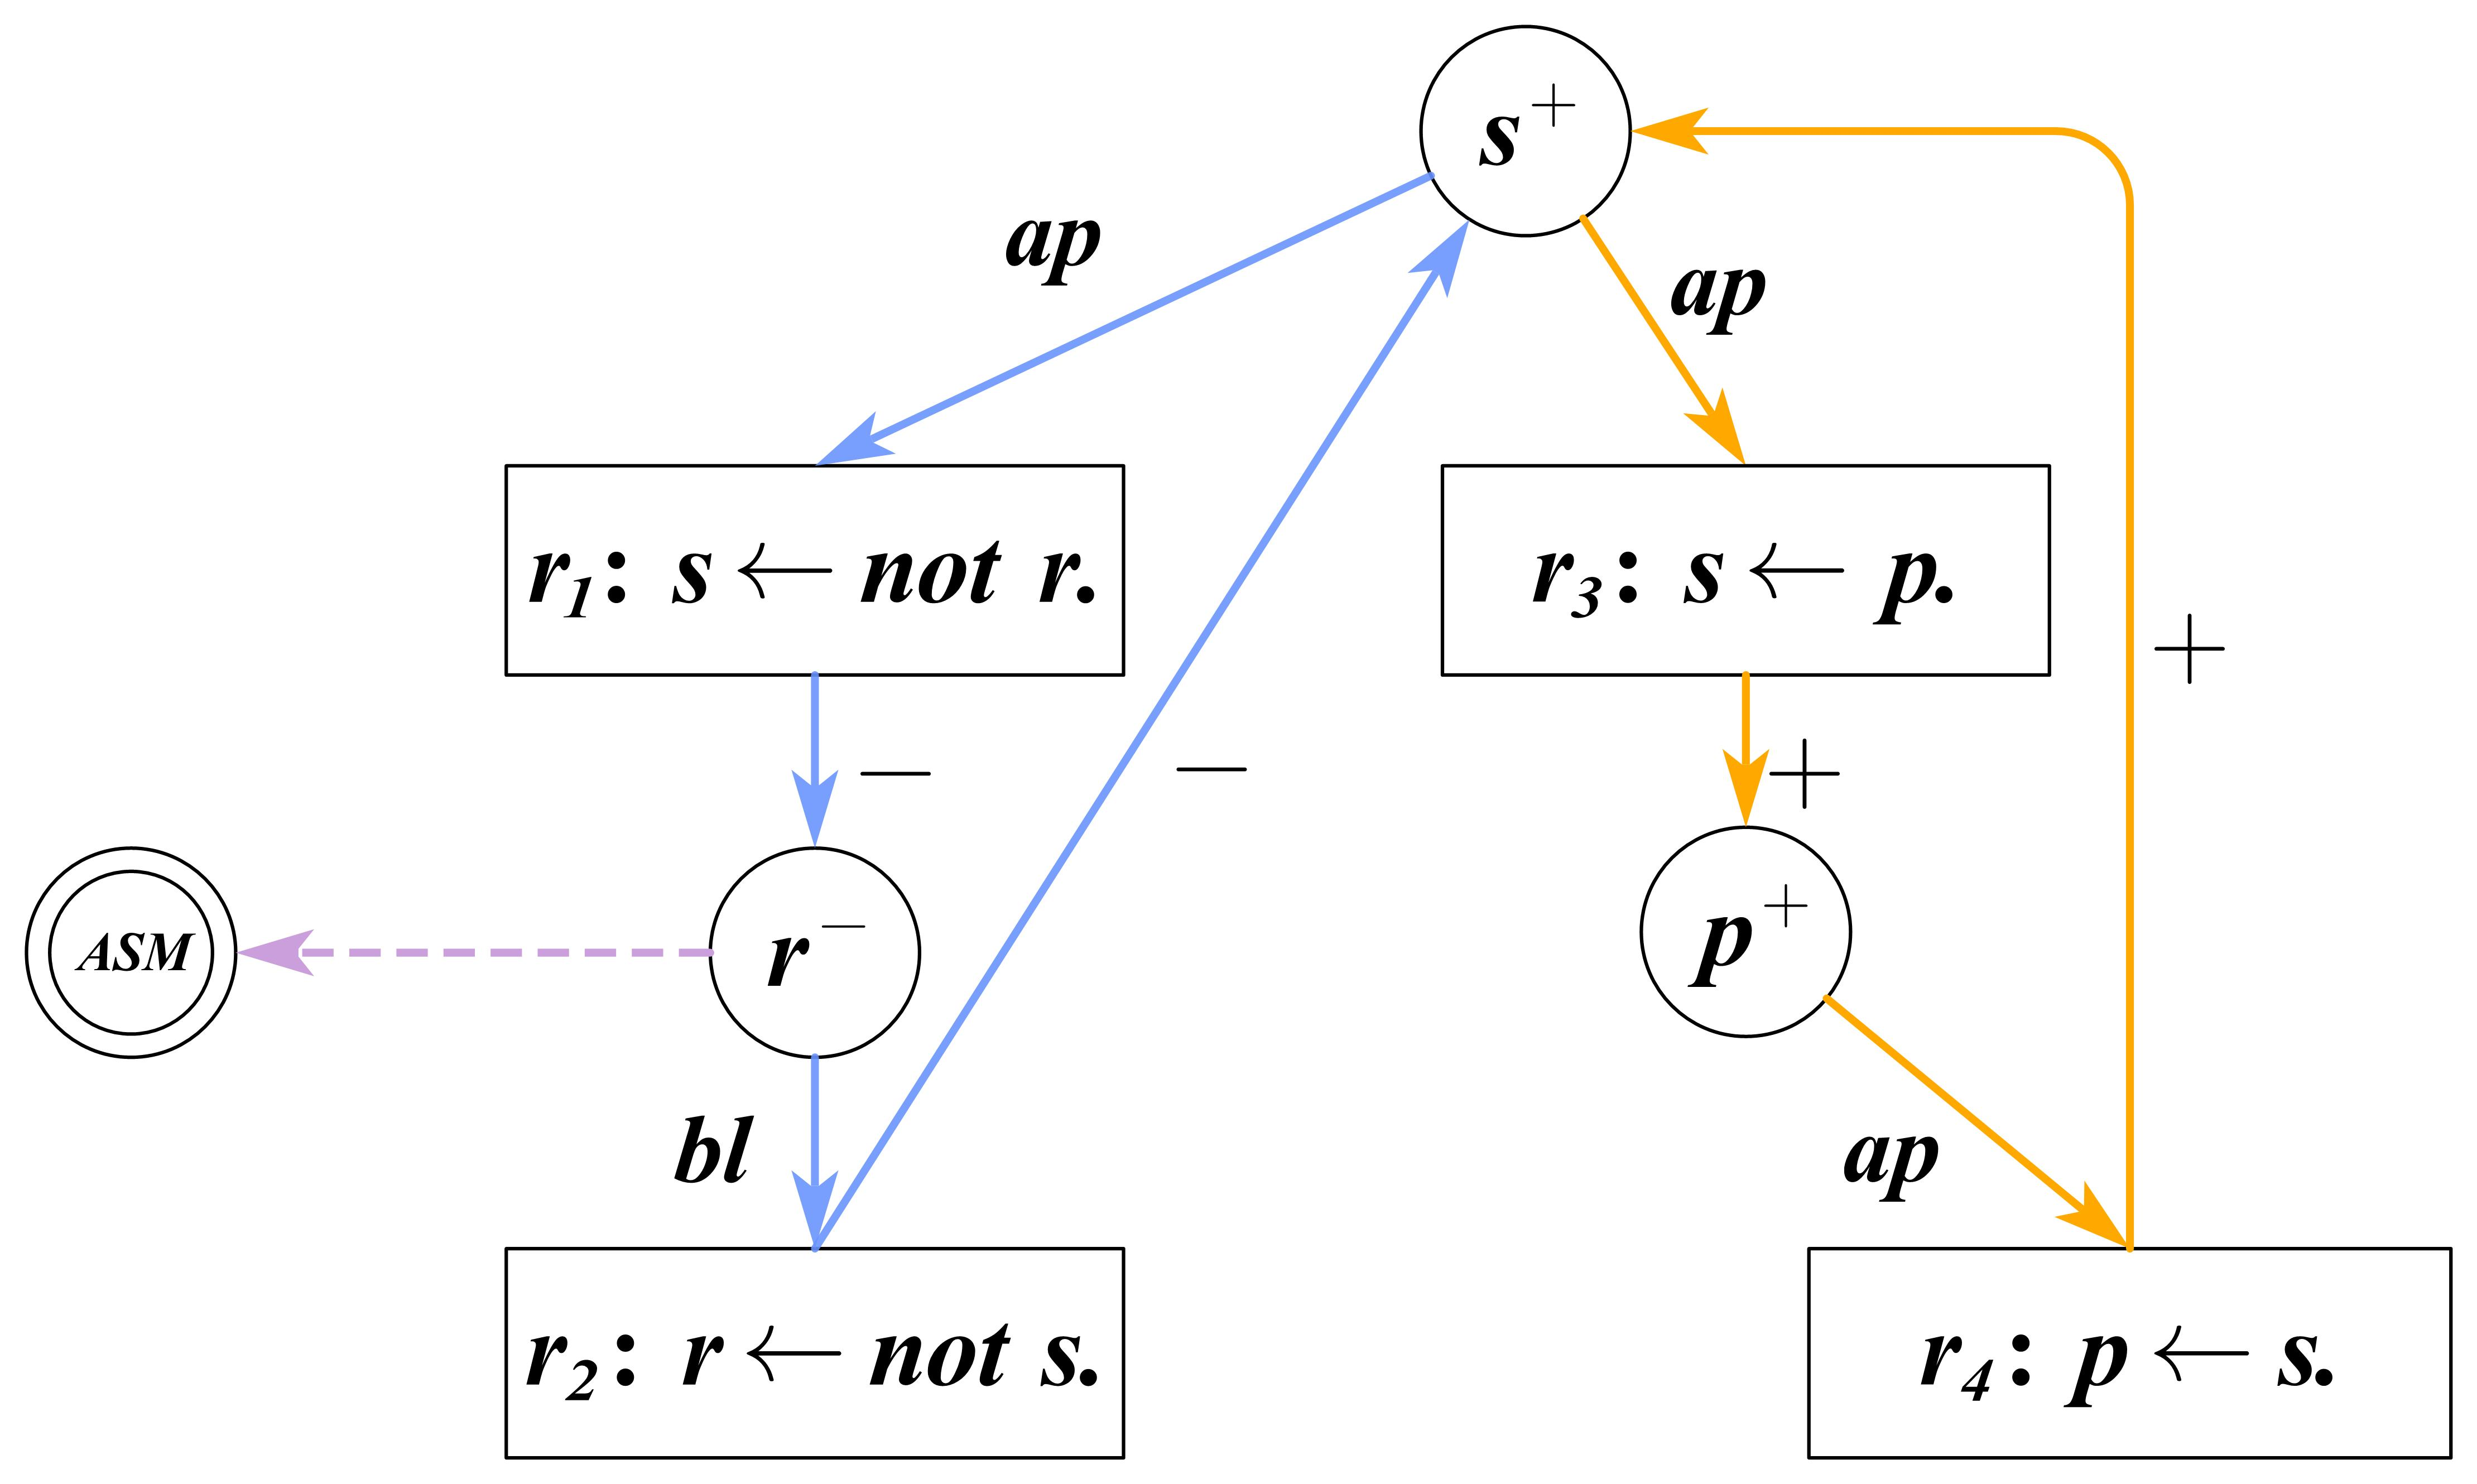
\includegraphics[height=.25\textwidth, valign=c]{figures/解释空间_2.jpg}} 
        \caption{程序\hyperref[prg:p_4]{$P_4$}在不同回答集与假设集下的两个解释空间}
        \label{fig:3_7}
    \end{figure}
    
    观察图\ref{fig:3_7}(a)可以发现,对于$s^-$而言,其真值为假既可以通过$s$位于“未受支持的正环”进行解释($UE$),也可以通过对其进行了为假的假设($ASM$)来解释。但是,通过进一步探究可以发现,正环未受支持,即规则$r_1$不适用,这一结论又需要通过$r^+$进行解释,而$r^+$再次通过规则$r_2$与$s^-$构成依赖关系。这一发现为后续构建解释时提供了一个重要的原则,即当某原子同时出现在未受支持的正环与负环中且其属于备选假设集合时,应当优先选择$ASM$进行解释。
\end{example}

\subsection{解释空间构建算法设计}
基于上述定义,下面给出解释空间生成的算法。本文的工作在花琪等人的解释空间\cite{huaqi2018lp}基础之上,重点增加了对解释空间中环处理的工作,其对应的流程如图\ref{fig:3_8}所示。
\begin{figure}[!h]
    \centering 
    \includegraphics[height=0.9\textwidth, valign=c]{figures/解释空间构建.jpg}
    \caption{程序\hyperref[prg:p_4]{$P_4$}在不同回答集与假设集下的两个解释空间}
    \label{fig:3_8}
\end{figure}

首先对ASP程序进行语法解析,构建文字结点集合$V_{atom}$、规则结点集合$V_{rule}$、汇结点集合$V_{sink}$,然后将其依赖关系通过规则适用边、原子依赖边、终结边进行连接形成图,并根据回答集对各结点与边进行正确的标记。进一步检测图中的环,若该环不存在出口,判定其为正环或负环,若为不存在出口的正环,判定其是否受到外部支持,若不受支持则将其中文字连接至$UE$结点;若为不存在出口的负环,计算可能的备选假设集,上述过程如算法\ref{alg:EU}所示。

\begin{algorithm2e}[H]
    \DontPrintSemicolon
    \SetKwInput{Initialization}{初始化}
    \SetKwInput{KwIn}{输入}
    \SetKwInput{KwOut}{输出}
    \setstretch{1.15}
    \caption{获取ASP程序$P$的解释空间}
    \label{alg:EU}
    \KwIn{一般ASP逻辑程序$P$,回答集$M \in SM(P)$}
    \KwOut{解释空间 $\mathit{EU_{P}=\langle V_{EU}, E_{EU} \rangle}$}
    \setcounter{AlgoLine}{0}
    \everypar={\nl}
    \Initialization{$V_{lit} = V_{rule} = E_{dep} = E_{end} \gets \phi$}
    \Initialization{$V_{sink} \gets \{ \text{\textit{Fact, NH, ASM, UE}}\}$}
    \ForEach{规则 $r$ 在 $P$所有规则中}{
      \If {$body(r) = \phi$}{
      $E_{end} =  E_{end} \cup (r, +, Fact)$
      }
      \If {$head(r)$不在$V_{EU}$中}{
        $V_{lit} = V_{lit} \cup head(r)$\;}
            \eIf {$M \models body(r)$}
                {$E_{ap} = E_{ap} \cup (head(r), ap, r)$\;}
            {
               $E_{ap} = E_{ap} \cup (head(r), bl, r)$ \;}
      \ForEach{文字$l$在\ $body(r)$中}{
        \If {$l \notin V_{lit}$}{
          $V_{lit} = V_{lit} \cup l$\;
        }
        \eIf {$l \in body^+(r)$}
        {$E_{dep} = E_{dep} \cup (r, +, l)$\;}
        {$E_{dep} = E_{dep} \cup (r, -, l)$\;}
      }
    }
    \ForEach {$v_{lit}$在$V_{lit}$中}{
        \If {$v_{lit}$ 出度为0}
            {$E_{end} = E_{end} \cup (v_{lit}, -, NH)$\;}
    }
    $cycles=$getAllCycles($V_{EU}$) // 找到当前图中的所有环集合cycles 
    \ForEach {$cycle$在所有环集合$cycles$中}{
    \If {$cycle$没有出口且为不被支持的正环}{
        \ForEach {$v_{lit}$在$cycle$中}
            {$E_{end} = E_{end} \cup (v_{lit}, -, UE)$}
    }
    \If {$cycle$没有出口且为不被支持的负环}
        {通过公式$\eqref{eq:asm}$计算$ASM$,由用户选择$U \in ASM$作为假设\;
        \ForEach {$v_{lit}$ in $U$}
           {$E_{end} \cup (v_{lit}, -, ASM)$}
        }
    }

    $V_{EU}=V_{lit} \cup V_{rule} \cup V_{sink}, E_{EU}= E_{dep} \cup E_{end}$\\
    \textbf{return} $\langle V_{EU}, E_{EU} \rangle$ 
\end{algorithm2e}


\section{ASP程序交互解释模型设计}
在定义了解释空间后,本文介绍对ASP程序交互解释模型的设计。下面首先通过给出该模型的输入与输出,定义可交互解释模型。
\begin{definition}[可交互解释模型]
    给定一个实例化、一致性ASP程序$P$及$P$的一个回答集$M$,$P$的解释模型$Exp_{cst}(P, s, INT(s))$有三个参数作为输入:
    \begin{itemize}[topsep=0pt]
        \setlength\itemsep{-0.3em}
        \item 实例化、一致性ASP程序$P$
        \item 当前解释步$s$,$s$是自然数
        \item 第$s$步的交互式信息$INT(s)$,这些信息包括:
        \begin{itemize}[label=$\circ$,topsep=0pt]
            \setlength\itemsep{-0.3em}
            \item 用户选择的稳定模型$M_s$,$M \in SM(P)$
            \item 用户当前步骤需要获取的解释$At_{exp_{s}}$,$At_{exp_{s}} \in Atom(P)$
            \item 用户选择的假设为假的集合$U_s$,$U_s \in Assumption(P, M)$
            \item 用户当前步骤选择展示的结点$v_s$,$v_s \in EU^{M, U}_P$
            \item 用户的当前步骤的退出信号$Q_s$,$Q_s \in \{true, false\}$
        \end{itemize}
    \end{itemize}
    
    上述符号中的下标$s$用于区分用户在不同交互步骤$s$下所提供的交互信息,这些交互信息满足如下约束:
    \begin{enumerate}[label=(\arabic*),topsep=0pt]
        \setlength\itemsep{-0.3em}
        \item $\forall i \ge 0, M_i = M_0, U_i=U_0, At_{exp_i}=At_{exp_0}$;
        \item $v_s \in \{v \mid v_{s'} \text{ 在第 }\ s' < s\ \text{ 步已经被选中,且边 }\ (v_{s'}, \cdot, v)\ \text{在}\ EU^{M, U_s}_P\ \text{中存在}\}$
    \end{enumerate}
    
    上述约束(1)表示在一次调试会话中,回答集、待解释原子和假设为假的集合被选定后,后续过程中将不再变化;约束(2)限制每一步能够被选择的结点只能是解释空间中与当前已展示出的结点一步可达的结点。

    该模型的输出$Exp_{cst}(P, s, INT(s))$如式\eqref{eq:expcst}所示:
    \begin{align}
        \label{eq:expcst}
        Exp_{cst}(P, s, INT(s))=
        \begin{cases}
        At_{exp_0} &s = 1, Q_s = false\\
        Exp_{cst}(P, s-1, INT(s-1)) &s > 1, Q_s = true\\
        Exp_{cst}(P, s-1, INT(s-1)) \cup v_s \cup Edge(v_s) & s > 1, Q_s = false\\
        \emptyset &\text{否则}\\
      \end{cases}
    \end{align}
    
    其中,$Edge(v_s)=\{(v_T, \cdotp, v_s) \mid v_T \in Exp_{cst}(P, s-1, INT(s-1)), (v_T, \cdotp, v_s) \in EU_{P}^{M,U}\}$
\end{definition}

由公式\eqref{eq:expcst}可以看出,该模型引入了解释步的概念,每一步都接受用户的一种选择,并指定用户当前关注的规则或文字。如果用户在当前步骤发送退出信号,或者如果没有其他有效节点可供用户选择,则该解释过程终止。实际上,交互式解释模型在任何步骤的输出都是解释空间的子图,并且解释构造的过程可以视为子图匹配。在这一过程中,对用户的引导和交互策略的设计至关重要。

接下来,本文具体讨论模型中的交互。模型中的交互的触发条件主要包括如下几个方面:
\begin{itemize}[topsep = 0pt]
    \item 解释开始前:
        \begin{enumerate}[label=(\arabic*), topsep = 0pt]
            \setlength\itemsep{-0.3em}
            \item 用户从多个回答集中选择指定的回答集;
            \item 用户从备选假设集合中选择指定的假设为假的原子集;
        \end{enumerate}
    \item 解释进行中:
       \begin{enumerate}[label=(\arabic*), topsep = 0pt]
            \setlength\itemsep{-0.3em}
            \item 当某条规则体部不唯一时,用户选择不同文字结点;
            \item 当某个文字位于多条规则头部时,用户选择不同的规则结点;
        \end{enumerate}
    \item 解释结束后:
        \begin{enumerate}[label=(\arabic*), topsep = 0pt]
            \setlength\itemsep{-0.3em}
            \item 用户对解释图进行存储和读取;
            \item 用户对得到的解释图进一步优化,仅查看适用的规则/阻塞的规则/最直接的文字依赖。
        \end{enumerate}
\end{itemize}

尽管用户可以在每一步骤下选择任何满足上述约束的节点,作为辅助工具,模型仍然希望通过引导与提示使得用户更便利地获取到交互解释。首先,由前面的定义和分析可以发现,假设集的概念对于用户而言并不直观。这一集合在图中体现为没有出口的负环,相较之下以图的形式对环进行展示,能够更直观准确地引导用户做出选择。另一方面,根据3.3.1中的分析可以知道,当某文字同时出现在未受支持的正环与负环中且其属于备选假设集合时,应当提示用户优先选择假设集作为解释。最后,从获取最直接解释的角度看,对于能够一步到达汇结点的文字,应当优先推荐用户查看与汇结点相连的解释。

\section{非实例化程序的变量处理}
上述对于ASP程序的解释的讨论,均面向实例化的ASP程序。但在实际应用中,程序中的变量是不可忽略的。本节讨论对非实例化程序中变量处理的方法,重点说明当前实例化工具面向解释的局限,同时给出解决这一局限性的方案。

\subsection{实例化工具\textsf{GRINGO}在ASP程序解释中的存在的问题}
为了获得一个实例化的程序,可以考虑直接采用现有的实例化工具(如\textsf{GRINGO}\cite{gebserGringoNewGrounder2007})。这些工具经过了多轮的版本迭代,不断优化\cite{gebser2011advances,gebser2015abstract},已经被稳定高效地应用于ASP程序的实例化问题中\cite{kaufmannGroundingSolvingAnswer2016}。

然而,在\textsf{GRINGO}的优化过程是面向求解的。通过\textsf{GRINGO}进行实例化得到的程序将会在保证回答集一致的情况下,被简化与改写。具体地,\textsf{GRINGO}对程序进行的简化包括:

\begin{itemize}[topsep = 0pt]
    \setlength\itemsep{-0.3em}
    \item 删除程序中体部不能被事实所满足的规则;
    \item 删除程序规则体部中能被事实满足的部分
\end{itemize}

\begin{example}[\textsf{GRINGO}的优化]
    考虑下面的非实例化程序$P_6$:
    \begin{align*}
        &r_1: fly(X) \leftarrow bird(X), not\ neg\_fly(X). \\
        &r_2: neg\_fly(X) \leftarrow penguin(X).\\
        &r_3: bird(tux).\\
        &r_4: bird(tweety).\\
        &r_5: penguin(tweety).
    \end{align*}
\end{example}

\begin{table}[!ht]
    \caption{程序$P_6$的预期实例化结果与在\textsf{GRINGO}实例化器下的实例化结果}
    \label{tb:3-1}
    \renewcommand{\arraystretch}{1.5}
    \begin{tabular}{ll}
    \hline
    期待的实例化结果$grd_{expect}(P_6)$ & \textsf{GRINGO}的实际输出$grd_{gringo}(P_6)$\tablefootnote{此处的执行的命令为: \texttt{gringo p\_6.lp -t --keep-fact}} \\ \hline
    \adjustbox{valign=t}{\begin{tabular}[c]{@{}l@{}}
        $fly(tux) \leftarrow bird(tux),$
        $\dashedbox{not\ neg\_fly(tux).}$\\ 
        $neg\_fly(tweety) \leftarrow penguin(tweety).$\\ 
        $\dashedbox{fly(tweety) \leftarrow bird(tweety), not\ neg\_fly(tweety).}$\\
        $\dashedbox{neg\_fly(tux) \leftarrow penguin(tux).}$
        \end{tabular} }
    &\adjustbox{valign=t}{ 
    \begin{tabular}[c]{@{}l@{}}
        $fly(tux) \leftarrow bird(tux).$\\
        $neg\_fly(tweety) \leftarrow penguin(tweety).$
    \end{tabular}
     } \\ \hline
    \end{tabular}
\end{table}

    该程序的唯一回答集为$M=\{bird(tux), bird(tweety), penguin(tweety),neg\_fly(twee\\\text{-}ty),fly(tux)\}$。从表\ref{tb:3-1}可以看出,由\textsf{GRINGO}得到的实例化程序与预期的实例化程序相比,第一条规则的负体部$not\ neg\_fly(tux)$被删除,三四两条规则整体没有出现在$grd_{gringo}(P_6)$中。为了更直观地说明这样的实例化为解释带来的困难,下面给出这两种实例化程序(在$M$下)对应的解释空间,如图\ref{fig:3_9}(a)与(b)所示。

    \begin{figure}[htbp] 
        \centering 
        \subfloat[$grd_{expect}(P_6)$在$M$下的解释空间]{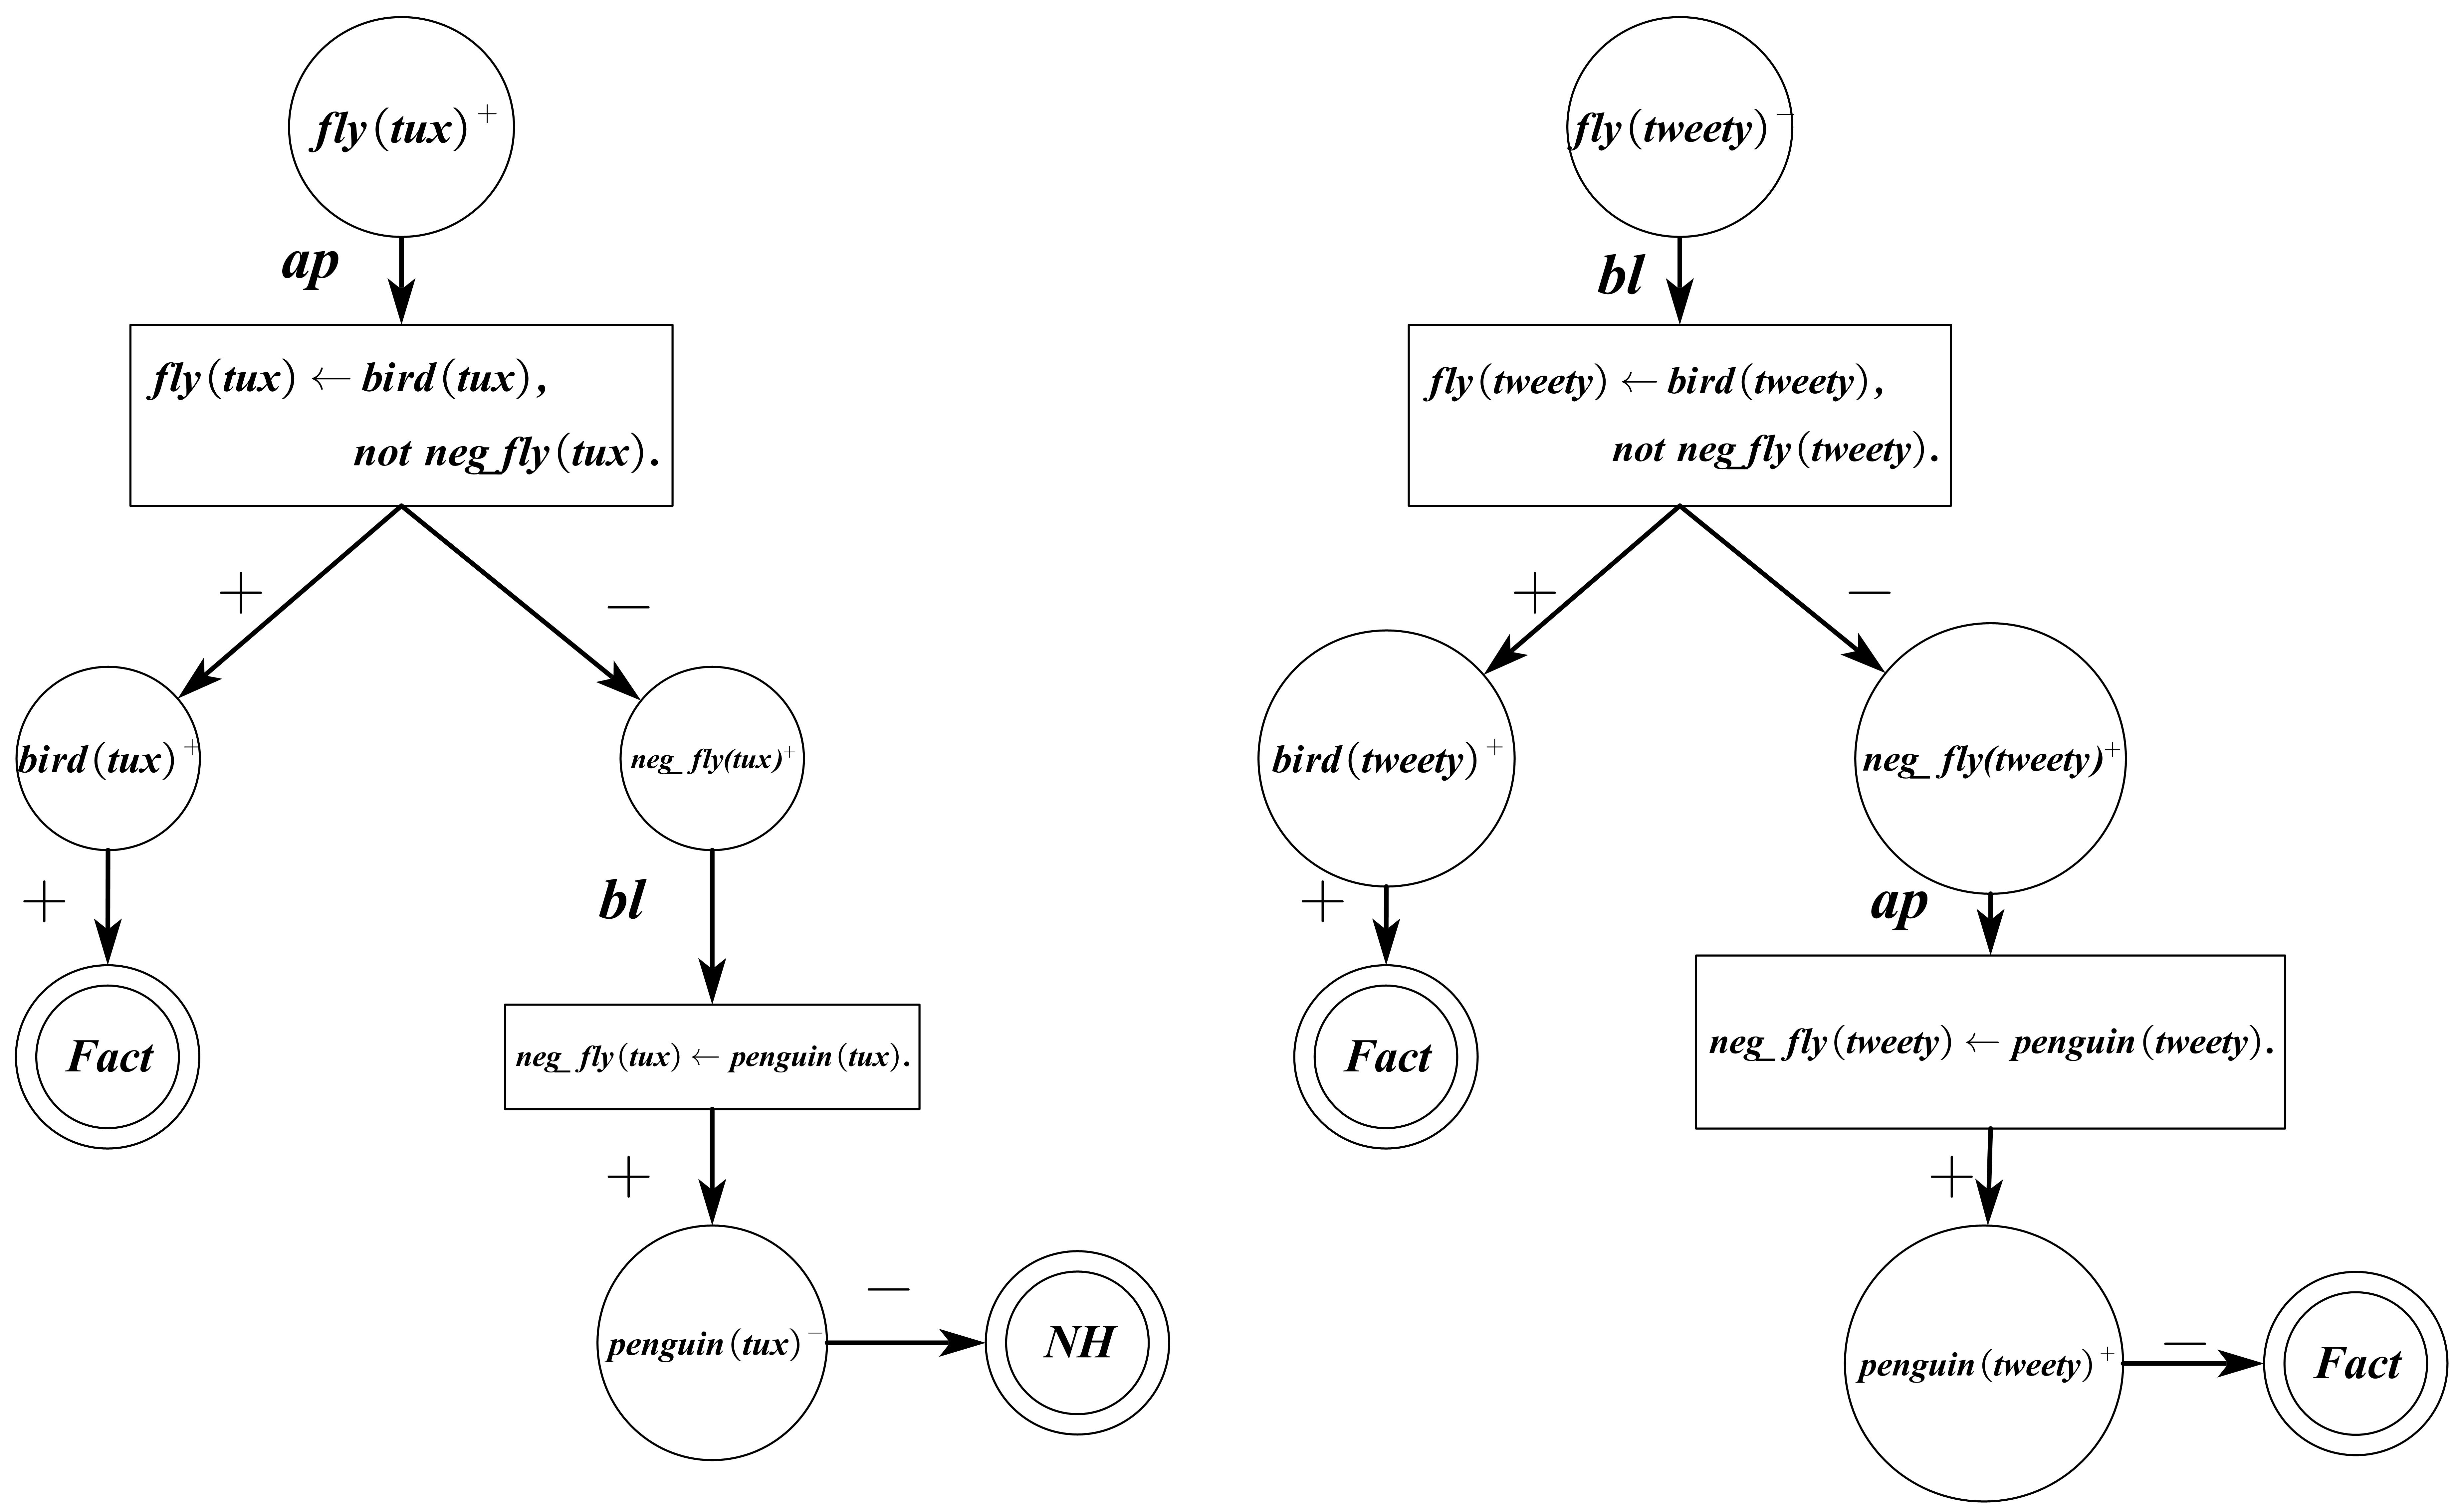
\includegraphics[height=.6\linewidth]{figures/p6解释空间-expect.jpg}} 
        \quad\quad
        \subfloat[$grd_{gringo}(P_6)$在$M$下的解释空间]{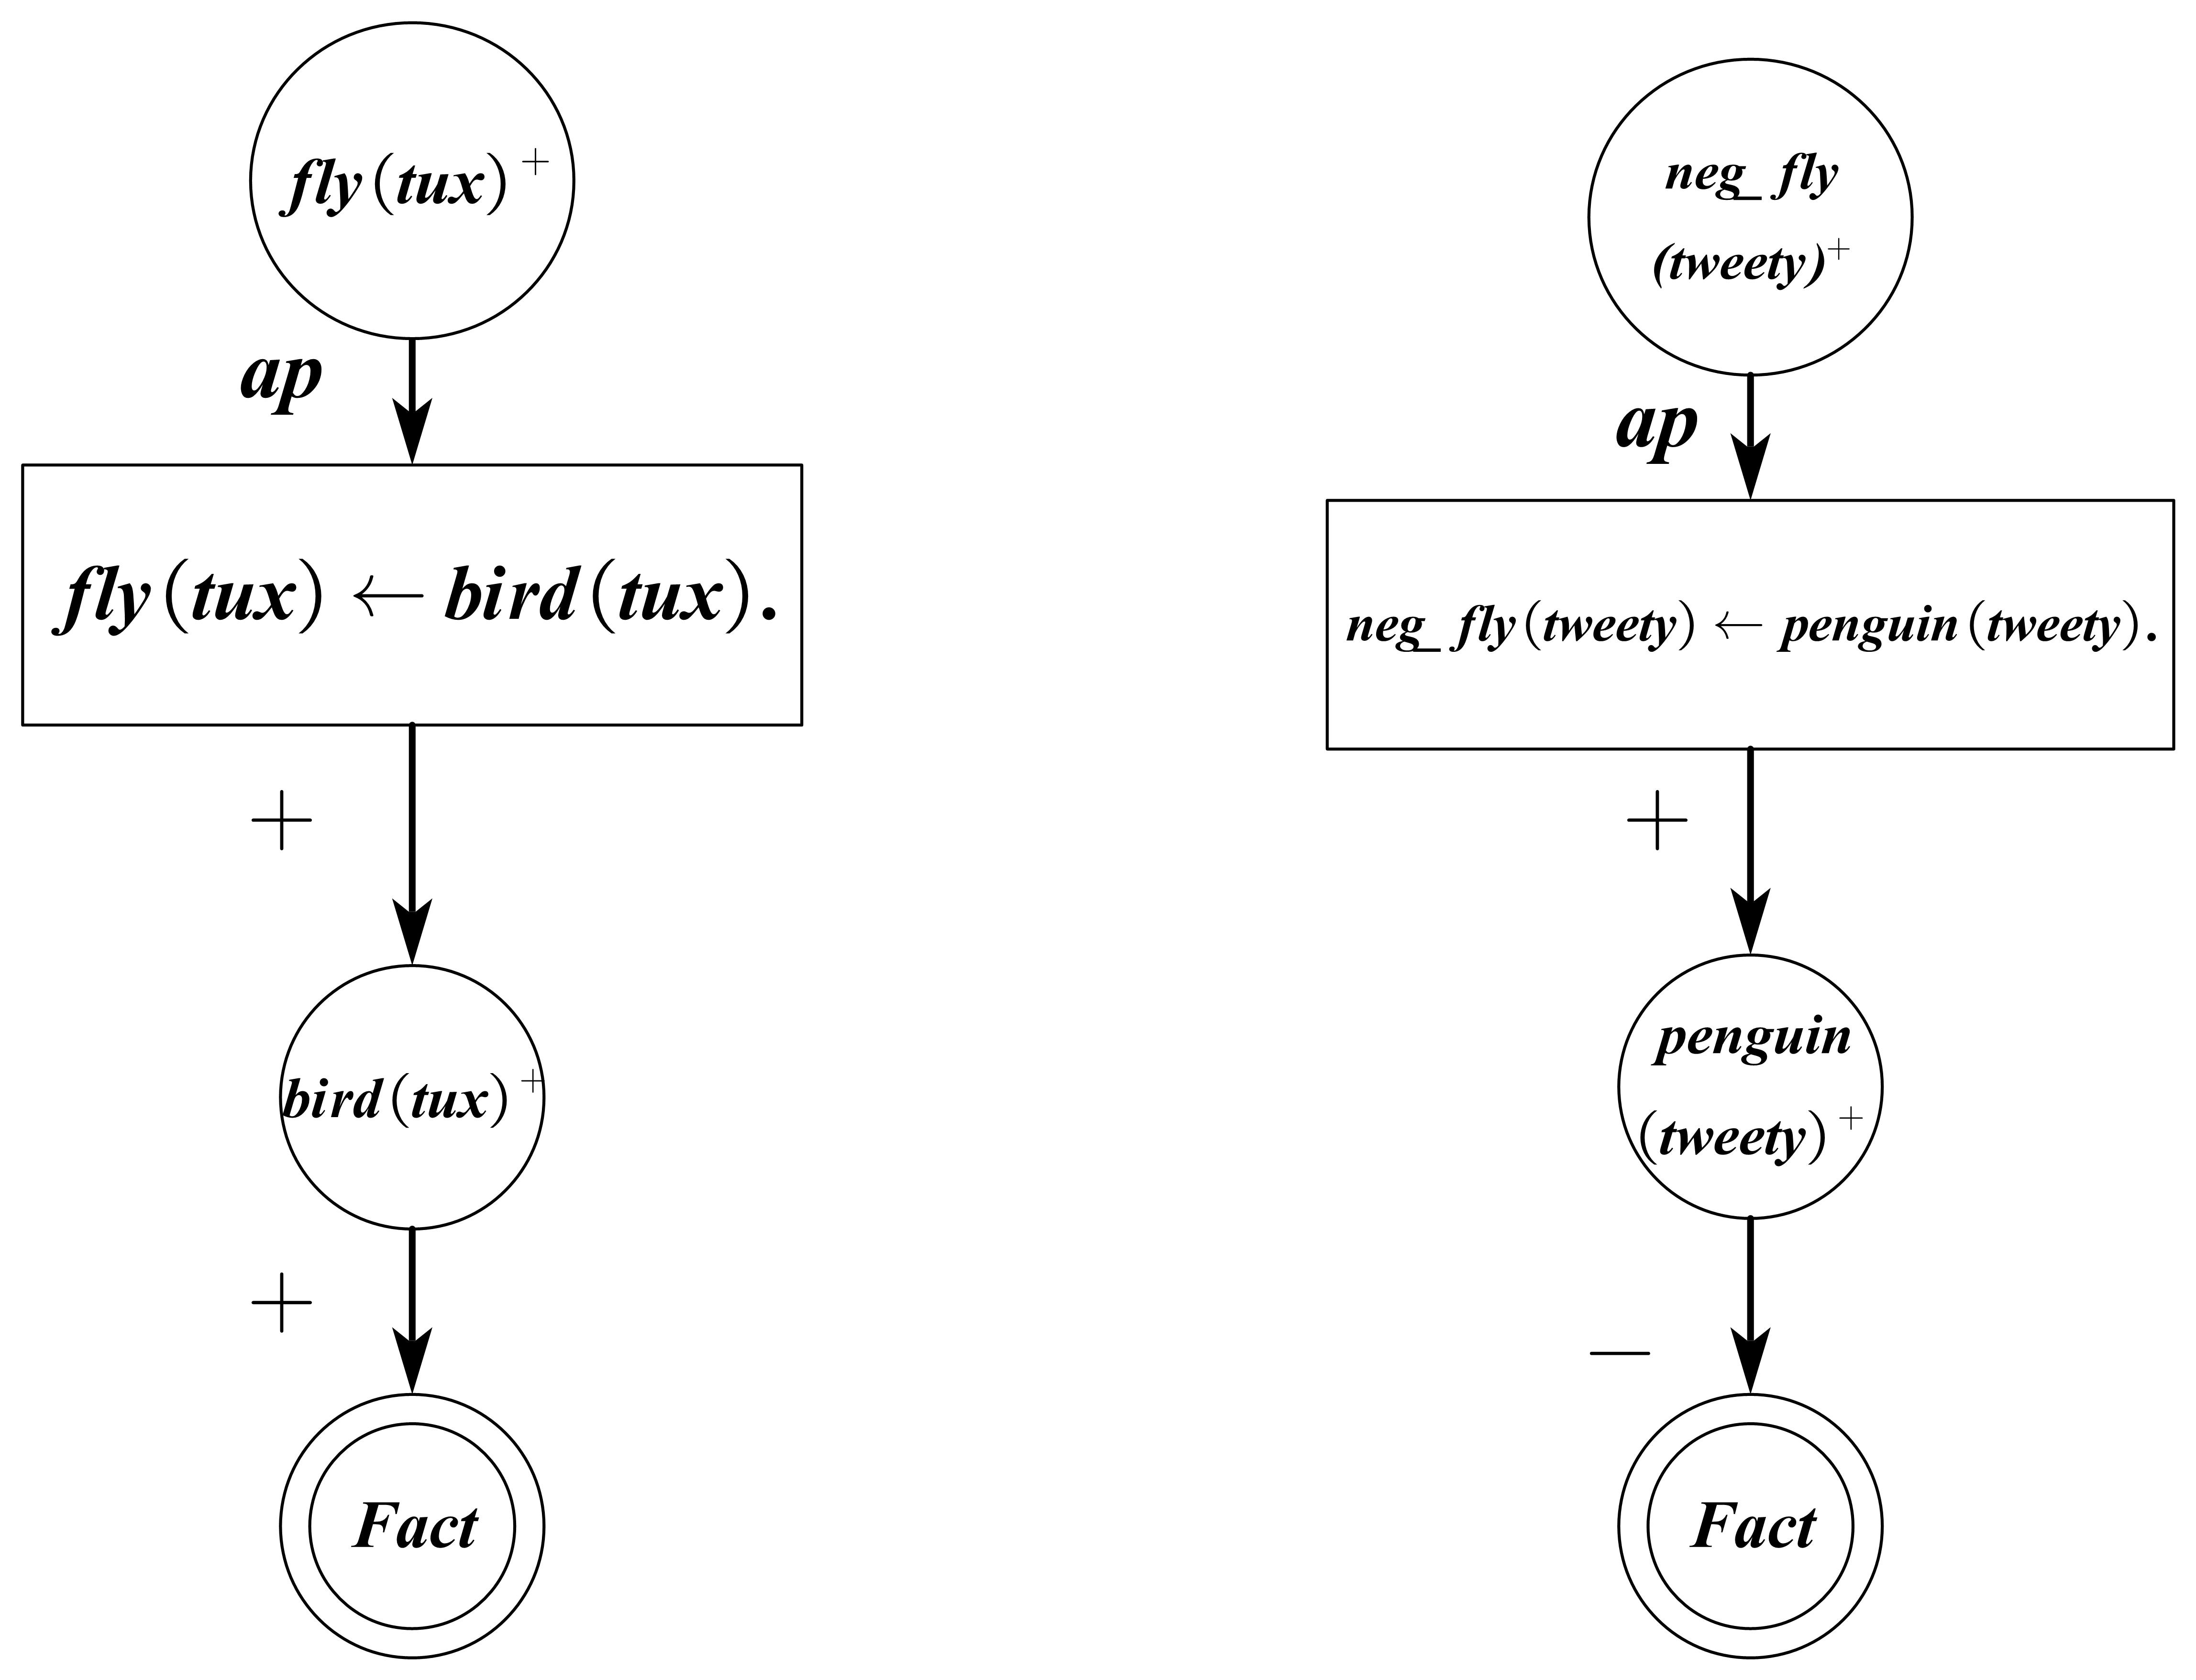
\includegraphics[height=.6\linewidth]{figures/p6解释空间-gringo.jpg}} 
        \caption{程序的两种图表示方法示意} 
        \label{fig:3_9} 
    \end{figure}

    很显然,当要求解释“\textbf{为什么tux能飞}”时,由\textsf{GRINGO}得到的实例化程序所构建的解释空间中,仅能解释为“\textbf{因为tux是鸟}”。而程序$P_6$的重点就是在于进行关于“\textbf{鸟类中不能飞的特例}”的推理,\textbf{解释tux能够飞还需要说明其不是鸟类中的特例},仅仅将“tux是鸟”作为解释显然是不够的,这一部分在$grd_{expect}(P_6)$中可以很好地得到解释;另一方面,对$tweety$来说,$grd_{gringo}(P_6)$得到的解释空间中甚至不包含$fly(tweety)$这一结点,更无从谈及对其进行解释。本文提出的解释,要求既能够对文字在回答集中的原因进行解释,也能够对不成立的文字进行解释。综上所述,由\textsf{GRINGO}得到实例化程序不能够满足本文对于解释的需求。

\subsection{基于元编程的交互式实例化方案}
    上文已经说明,\textsf{GRINGO}的版本迭代与优化已经使其具有高性能的实例化能力,因此本文仍然采用该工具进行实例化。在明确了部分规则与规则中的文字被简化或删除的原因后,通过元编程的方式,枚举每条规则体部的可满足性情况,通过编写一个上层的ASP程序,在对应的回答集中找出完整的实例化结果。为了实现对于程序的转换,参考Brain等人在\textsf{SPOCK}中的Kernel Transformation,下面给出定义程序$P$的核变换。

    \begin{definition}[程序$P$的核变换$\mathcal{K}$]
        给定一个非实例化的ASP程序$P$,$r$是$P$中的一条非事实规则($body^+(r) \cup body^-(r) \neq \emptyset$):
        \begin{align}
            \mathbf{head(r)} \leftarrow \mathbf{  body^+(r), \text{not } body^-(r)} 
        \end{align}
        
        其中,$\mathbf{head(r), body^+(r), body^-(r)}$分别表示规则$r$的头部、正体部和负体部。该规则的核变换$\mathcal{K}(r)$定义为:
        \begin{align}
            \mathcal{K}(r)= K_{ap}(r) \cup K_{blp}(r) \cup K_{bln}(r)
        \end{align}
        其中:
        \begin{align}
            &K_{ap}(r)=ap(head(r), p(body^+(r)), n(body^-(r))) \leftarrow body^+(r), not\ body^-(r) \label{eq:kap}\\
            &K_{blp}(r)=\bigcup\limits_{{l \in body^+(r)}} \left(bl(head(r), p(body^+(r)), n(body^-(r)))\leftarrow not\ l, var(X) \right) \label{eq:blp}\\
            &K_{bln}(r)=\bigcup\limits_{{l \in body^-(r)}} \left(bl(head(r), p(body^+(r)), n(body^-(r)))\leftarrow l, var(X) \right) \label{eq:bln}
        \end{align}
        则程序$P$的核变换$\mathcal{K}(P)$定义为:
        \begin{align}
            \mathcal{K}(P) = \left( \bigcup_{\substack{r \in P,\\body^+(r) \cup body^-(r) \neq \emptyset}}\mathcal{K}(r) \right) \cup P
        \end{align}
    \end{definition}

    \begin{theorem}[程序的核变换有且仅有一个回答集]
        \label{thm:kernel}
        给定一个ASP程序$P$, 其核变换$\mathcal{K}(P)$ 有唯一回答集。
    \end{theorem}

    \begin{proof}[定理\ref{thm:kernel}的证明]
        $\forall r' \in \mathcal{K}(P), head(r') \in \{ap/3, bl/3\}$, 且 $body(r') \cap \{ap/3, bl/3\} = \phi$, 因此$\mathcal{K}(P)$不包含环。 Kunen等人提出不包含环的ASP程序称为调用一致性程序(call-consistent)\cite{kunen1989signed}。 Papadimitriou等人证明了调用一致性ASP程序有且仅有一个回答集\cite{PAPADIMITRIOU199748},因此定理\ref{thm:kernel}成立。
    \end{proof}

    式\eqref{eq:kap}-\eqref{eq:bln}是核变换的三组核心规则,这三组规则实际上枚举了一条ASP规则体部的三种满足性情况:同时满足正体部与负体部、不满足正体部、不满足负体部。在这样的情况下,无论程序中的事实如何,对事实中的每一个对象常量$c$和程序中的每一个非事实的实例化规则$r$而言,一定能找到规则$r' \in \mathcal{K}(r)$,使得$c$被实例化进入$r'$体部的项中。

    \begin{example}[程序$P_6$的核变换]
        为程序$P_6$进行核变换,得到的$\mathcal{K}(P_6)$为:
        \begin{align*}
            &fly(X) \leftarrow bird(X), not\ neg\_fly(X).\\
            &\dashedbox[colback=gray!30]{ap(head(fly(X)), p(bird(X)), n(neg\_fly(X))) \leftarrow bird(X), not\ neg\_fly(X).}\\
            &\dashedbox[colback=gray!30]{blp(head(fly(X)), p(bird(X)), n(neg\_fly(X))) \leftarrow not\ bird(X), var(X).}\\
            &\dashedbox[colback=gray!30]{bln(head(fly(X)), p(bird(X)), n(neg\_fly(X))) \leftarrow neg\_fly(X).}\\
            &neg\_fly(X) \leftarrow penguin(X).\\
            &\dashedbox[colback=gray!30]{ap(head(neg\_fly(X)), p(penguin(X)), n()) \leftarrow penguin(X).}\\
            &\dashedbox[colback=gray!30]{blp(head(neg\_fly(X)), p(penguin(X)), n()) \leftarrow not\ penguin(X), var(X).}\\
            &bird(tux;tweety).\\
            &penguin(tweety).\\
            &var(tux;tweety).
        \end{align*}
    
        $\mathcal{K}(P_6)$的回答集中关于原子ap、blp和bln的文字为:
    \begin{align*}
        \{&ap(head(neg\_fly(tweety)),p(penguin(tweety)),n),\\
        &ap(head(fly(tux)),p(bird(tux)),n(neg\_fly(tux))),\\
        &bln(head(fly(tweety)),p(bird(tweety)),n(neg\_fly(tweety))),\\
        &blp(head(neg\_fly(tux)),p(penguin(tux)),n)\}
    \end{align*}
    
    逐条对上述文字中的head项、p项和n项中的项进行提取,可以得到对应的完整实例化程序:
    \begin{align*}
        &neg\_fly(tweety) \leftarrow penguin(tweety).\\
        &fly(tux) \leftarrow bird(tux), neg\_fly(tux).\\
        &fly(tweety) \leftarrow bird(tweety), neg\_fly(tweety).\\
        &neg\_fly(tux) \leftarrow penguin(tux).
    \end{align*}
    \end{example}

    然而,上述方案在实现过程中可能出现空间复杂度过大的问题。对于一个有$n$个变量的ASP程序,假设不同的对象常量数量为$c$,那么所有不同的实例化替换的方式理论上有$n^c$个,而实际上有些实例化在应用中是冗余的。考虑程序$P_6 \cup \{cat(elvis).\}$。此时,$elvis$作为猫的名字,与整个程序$P_6$所讨论的物种不再相关,因此将其放入实例化程序中似乎没有必要。但是,用户依然有可能寻求解释:\textbf{为什么elvis不会飞?}。此时,仍需要借助规则$fly(elvis) \leftarrow bird(elvis), neg\_fly(elvis).$来进行解释。因此,考虑通过在实例化前进行用户交互,进一步缩减实例化规模。注意到上文中,增加了一个辅助文字$var$,这一文字用于保证Clingo语法下规则的安全性(Safety)。具体来说,所谓安全的规则,是指出现在规则负体部的文字必须至少在头部或正体部内也出现一次\cite{calimeri2020aspcore2}。而在核变换中对正体部错误情况进行枚举时,将会出现规则仅有一个负体部的情况。此时,若用户能够指定一个“最基础的谓词”,满足“违背该谓词的情况不予考虑”,则能够降低程序的规模。例如,若用户指定违背$bird(X)$的情形不予考虑,那么上述程序中$not\ bird(X)$的规则阻塞情况将不会被枚举。另一方面,在Yuanlin Zhang等人提出的基于ASP的扩展语言\textsf{onlineSPARC},面向ASP程序的教学,通过引入了sort的概念,在程序编写时为每个变量都明确指定了最基本的域\cite{marcopoulos2019onlinesparc, balai2013answer}。本文借鉴这一工作的思路,若用户指定了最基础谓词,则继续考虑将其他谓词与之绑定。例如$neg\_fly(X)$中的$X$一定也满足$bird(X)$,以避免出现将elvis(猫名)带入关于鸟的规则中进行讨论的冗余情况出现。


    \section{本章小结}
    为了给出一个用户可接受且清晰完整的ASP回答集文字的解释,本章提出了一个基于用户交互的ASP程序解释模型并给出其构建算法。为了构建这一模型,首先对已有工作进行改进,找到了一种合适的ASP程序图表示方法——扩展文字-规则图,然后重点对图中的环进行处理,以得到ASP程序的解释空间并给出其构建算法;进一步,基于解释空间形式化定义交互解释模型并探究用户交互解释的过程,最后针对非实例化程序,研究当前实例化工具在进行解释任务中存在的局限性,通过元编程的方法给出面向解释的ASP程序实例化方案。
\chapter{ASP程序调试模型的设计}
\label{chp:debug}
在定义了ASP程序的解释模型后,本节将基于该解释模型,进一步定义ASP程序的调试模型。考虑ASP程序的调试场景,大致可以分为两种不同的情况:
\begin{enumerate}[topsep=0pt]
    \setlength\itemsep{-0.3em}
    \item 程序是一致的,但用户预期出现(不应出现)的文字未出现(出现)在回答集中;
    \item 程序是不一致的,但没有回答集或回答集为程序中所有的文字\cite{schulz2015characterising}。
\end{enumerate}
现有调试研究主要集中对不一致程序进行,因此本章首先介绍不一致逻辑程序的模型,然后再介绍一致性程序调试模型。
\section{不一致ASP程序的调试}
对于不一致的ASP程序,其调试的难点通常在于面对\textit{UNSATISFIABLE}的求解结果,即使用户心中已有明确期待的一个或多个回答集文字,程序的问题也不一定出现与这些文字在相关的规则或事实中,也可能是其他部分的矛盾导致了整个回答集都无法获得。当程序规模较大或程序逻辑较为复杂的时候,用户只能试探性地猜测可能出现问题的规则将其从程序中删除,再尝试对剩余部分求解。这样的行为效率较低,并且删除掉的规则未必就是存在问题的规则。因此,亟需在程序编写完成后对其进行一个静态分析,以快速定位导致程序不一致问题的文字,提示用户对包含这些文字(及其关联规则)重点关注,推荐作为调试的入口;另一方面,为了更真实地将命令式语言的调试风格引入ASP程序,考虑设计一个单步调试模型,使得规则间无序的ASP程序在用户的交互下按照交互步有序执行,直到发现程序中的问题。本节分别介绍基于程序静态分析的调试入口推荐和不一致ASP程序的单步调试模型设计。
\subsection{基于程序静态分析的调试入口推荐}
对不一致ASP程序的研究已经有很多丰富的结论,其中Schulz等人对不一致程序给出了三种情形的讨论\cite{schulz2015characterising},全面系统地找到了导致ASP程序不一致的原因。该讨论基于良基模型,并且能够指出程序中造成不一致的“元凶文字集(Culprit Set)”。这一过程可作为ASP程序调试模型中调试前进行的一次静态程序分析,并且该过程不依赖于回答集。根据是否具有良基模型,下面将介绍这三种原因,之后进一步详细讨论造成不一致的具体文字或规则,并基于这三种原因给出基于程序静态分析的调试入口推荐算法。
\subsubsection{不一致程序的三种情形}
实际上,程序中的“否定”(包括强否定与NAF否定)是造成逻辑程序不一致的根本原因。Gelfond与Lifschitz等人已经证明,如果一个逻辑程序不含这两种否定,该程序在稳定模型语义下一定是一致的\cite{gel91b}。对于存在否定的程序,其不一致原因的产生又可以归因于两种情况:1)回答集是程序中全部的文字;2)程序不存在回答集。通过考察程序的良基模型,这两种情况进一步又可以细分为如下3种情景,下面分别通过例子加以说明。

\subsubsection*{情形1:程序$P$没有良基模型,且程序的唯一回答集是$Lit(P)$}
\begin{example}[程序$P_7$]
    \label{eg:4.1}
    考虑下面的一个不一致程序$P_7$ \label{prg:p7}:
    \begin{center}
        \begin{tabular*}{.8\linewidth}{l @{\extracolsep{\fill}} lll}
            $r_1: p \leftarrow q.$ & $r_2: q \leftarrow r.$ & $r_3: r \leftarrow.$ & $r_4: s \leftarrow.$ \\
            $r_5: u \leftarrow not\ t.$ & $r_6: t \leftarrow not\ u.$ & $r_7: \lnot p \leftarrow.$ & 
        \end{tabular*}
    \end{center}
    
    程序\hyperref[prg:p7]{$P_7$}没有良基模型。假设其存在回答集$S$,由于程序中的三条事实$r_3, r_4, r_7$,可得到$r \in S, s \in S, \lnot p \in S$。进一步根据$r_1, r_2$,得到$q \in S, p \in S$,此时$S$中包含了一对互补文字$p, \lnot p$,根据回答集的定义可以得到,若$P_7$存在回答集,则回答集必须是程序中的所有文字,即$S=Lit(P_7)$。又因为$\forall r \in P_7^{Lit(P_7)}, S'=\{p, \lnot p, q, r, s\} \models r$,且不存在$S'' \subset S'$满足程序$P_7^{Lit(P_7)}$的所有规则,而$S'$依然包含互补文字$p, \lnot p$,因此$Lit(P_7)$就是$P_7^{Lit(P_7)}$的回答集,进一步得到$Lit(P_7)$是$P_7$的回答集。可以看到,NAF文字的负环($r_5, r_6$与$u, t$)在这里并没有直接导致不一致的出现,从上述的推导过程可以看到,这个程序不一致的直接原因是$\lnot p$与$p$分别通过不含NAF的规则被蕴含。
\end{example}

\subsubsection*{情形2:程序$P$没有良基模型,同时没有回答集}
\begin{example}[程序$P_8$]
    \label{eg:4.2}
    考虑下面的一个不一致程序$P_8$ \label{prg:p8}:
    \begin{center}
        \begin{tabular*}{.8\linewidth}{l @{\extracolsep{\fill}} ll}
            $r_1: q \leftarrow not\ r.$ & $r_2: \lnot q \leftarrow \lnot s, not\ p.$ & $r_3: r \leftarrow not\ \lnot t$\\
            $r_4: \lnot s \leftarrow.$ & $r_5: \lnot t \leftarrow.$ &
        \end{tabular*}
    \end{center}
    
    程序\hyperref[prg:p8]{$P_8$}没有良基模型。假设其存在回答集$S$,由于程序中的事实$r_4, r_5$,可得到$\lnot s \in S, \lnot t \in S$。进一步根据$r_1, r_2, r_3$,得到$\lnot q \in S, q \in S$。此时$S$中包含了一对互补文字$q, \lnot q$,根据回答集的定义可以得到,若$P_8$存在回答集,则回答集必须是程序中的所有文字,即$S=Lit(P_8)$。而$P_8^{Lit(P_8)}=\{q \leftarrow ., \lnot s \leftarrow., \lnot t \leftarrow.\}$,该程序的回答集$\{q, \lnot s, \lnot t\}$中不包含互补文字,因此,$Lit(P_8)$不是$P_8$的回答集,这与假设矛盾,程序\hyperref[prg:p8]{$P_8$}没有回答集。与上例不同的是,此处造成不一致的地方虽然也是互补文字($q, \lnot q$),但推出这一对文字的规则中均包含NAF。
\end{example}

因此,上述两种情景中,情景1的不一致归因于其包含的强否定,而情景2的不一致则同时归因于强否定与NAF。事实上,对于没有良基模型的ASP程序$P$而言,有如下定理:

\begin{theorem}
    给定一个回答集程序$P$,若$P$没有良基模型,$\vdash_{MP}$表示命题逻辑推理中的假言推理(modus ponens),推理结论仅使用程序中的$\leftarrow$作为规则得到,则:
    \begin{enumerate}[itemsep=0pt, label=(\arabic*)]
        \item $P$的回答集是$Lit(P)$,当且仅当$\exists a \in HB_P$,使得$P \vdash_{MP} a$且$P \vdash_{MP} \lnot a$,
        \item $P$没有回答集,当且仅当$\nexists a \in HB_P$,使得$P \vdash_{MP} a$且$P \vdash_{MP} \lnot a$。
    \end{enumerate}
\end{theorem}
    注意到例\ref{eg:4.2}中$\lnot q$的推导需要$not\ p$的成立,而$not\ p$是通过“$p$未出现在任何规则头部无法推导”推理得到,因此$P_8 \not\vdash_{MP} \lnot q$,而$P_8 \cup \{not\ p\} \vdash_{MP} a$。本文借用Schulz等人的定义,对于ASP程序$P$及其中的一个文字$a$,若$P \vdash_{MP} a$,则$a$能够被$P$\textbf{严格推出(strictly derivable)};若$P \not\vdash_{MP} a$,但$\exists \Delta\subseteq NANT(P), P \cup \Delta \vdash_{MP} a$,则$a$能够被$P$\textbf{可废止推出(defeasibly derivable)}。例\ref{eg:4.1}中,$\lnot p$被程序$P_7$严格推出,而例\ref{eg:4.1}中,$\lnot q$被程序$P_8$可废止推出。

\subsubsection*{情形3:程序$P$有良基模型,但没有回答集}
\begin{example}[程序$P_9$]
    \label{eg:4.3}
    考虑下面的一个不一致程序$P_9$ \label{prg:p9}:
    \begin{center}
        \begin{tabular*}{.8\linewidth}{l @{\extracolsep{\fill}} ll}
            $r_1: r \leftarrow not\ s.$ & $r_2: q \leftarrow not\ s.$ & $r_3: p \leftarrow not\ r.$\\
            $r_4: s \leftarrow not\ r.$ & $r_5: \lnot q \leftarrow not\ s.$ & $r_6: \lnot p \leftarrow not\ r.$
        \end{tabular*}
    \end{center}
    
    程序\hyperref[prg:p9]{$P_9$}有良基模型$\langle \emptyset, \emptyset \rangle$。该程序没有回答集,假设其存在回答集$S$,观察各规则可以发现,文字$s, r$有且仅有一个会出现在$S$中。若$s \in S$,则$p, \lnot p \in S$;若$r \in S$,则$q, \lnot q \in S$,因此$S$只可能是$Lit(P_9)$。又由于$P_9^{Lit(P_9)}=\emptyset$,因此$P_9^{Lit(P_9)}$的唯一回答集为$\emptyset \subset Lit(P_9)$,$Lit(P_9)$不是$P_9$的回答集,进而得到$P_9$没有回答集。与例\ref{eg:4.2}不同的是,此处导致互补文字出现的虽然仍NAF导致,但NAF成立的条件为程序中的负环($r_1, r_4\ \text{与 }\ s, r$)。
\end{example}

\subsubsection{导致程序不一致的具体文字集合}
在上述三种情形的讨论中,已经以非形式化的说明分析了导致三类不同的程序出现不一致的具体文字。与本章开头的结论相一致,两类否定,即强否定与NAF是造成程序不一致的唯一可能原因。下面以定理的方式形式化地给出导致三类程序不一致的文字集合结论,其中第三类程序需要分两种情况讨论,定理的证明见附录。

\begin{theorem}
    \label{thm:incstlit}
    对一个非一致性ASP程序$P$,$P'$通过将$P$中所有的强否定文字$\lnot a$替换为$a'$得到的一个转换程序,$INCST(P)$为直接导致其不一致的文字集合,$\langle WF^+_{P'}, WF^-_{P'} \rangle$则:
    \begin{enumerate}[itemsep=0pt, label=(\arabic*)]
        \item $P$无良基模型,唯一回答集为$Lit(P)$:
        $$INCST(P)=\{a, \lnot a\ \mid (a, a' \in WF^+_{P'}) \land (P' \vdash_{MP} a) \land (P' \vdash_{MP} a')\}$$
        \item $P$无良基模型,无回答集:
        $$INCST(P)=\{a, \lnot a\ \mid a\ \text{或} a' \text{被程序} P' \text{可废止推出}\}$$
        \item $P$有良基模型(无回答集),但$P'$有回答集$S'$:
        $$INCST(P)=\{a, \lnot a\ \mid (a, a' \in S'), a\ \text{或} a' \text{被程序} P' \text{可废止推出}\}$$
        \item $P$有良基模型(无回答集),但$P'$没有回答集$S'$:
        $$INCST(P)=\{b_1, \ldots, b_o, b_1\ \mid (b_1, \ldots, b_o, b_1) \in cyc^-(P), b_i\ \text{不在程序的三值模型中}\}$$
    \end{enumerate}
\end{theorem}

根据上述四个定理,本文对用户输入的程序进行一次静态分析,判断程序不一致落入何种情形,并给出导致其不一致的直接文字集合。进一步,对于不一致程序而言,虽然不存在解释空间(由于没有一致回答集),但可以构建其原子-规则图$ARG$,将包含导致不一致的直接文字集合的最小子图从原子-规则图ARG中提取出来,提示用户需要检查的规则和原子;另一方面,相较于命令式语言的程序,声明式语言程序没有明确的程序入口和执行次序,第三章中的解释模型将“步”的概念引入解释中,因此考虑进一步将其引入调试中,这要求用户指定一个调试的起点(入口),上述定理得到的$INCST$集合可作为用户调试入口的推荐,引导用户从这些文字出发,更快地找到程序的错误。图4-1给出了查找直接导致不一致集合的流程示意图。
\begin{figure}[htbp]
    \centering
    \includegraphics[height=.8\textwidth, valign=c]{figures/不一致集合计算.jpg}
    \caption{不一致集合计算流程示意}
\end{figure}

对于前三种情况,推荐用户直接以$INCST$集合中的文字作为调试起点,并利用下文介绍的调试模型进行调试;对于第四种情况,除了给出$INCST$集合外,还将原子-规则图中的相关奇数负环找出,以供用户在调试前对相关规则进行检查,向用户推荐调试入口的过程如算法\ref{alg:dbgetcrcmd}所示。

\begin{algorithm2e}[H]
    \label{alg:dbgetcrcmd}
    \DontPrintSemicolon
    \SetNoFillComment
    \SetKwInput{Initialization}{初始化}
    \SetKwInput{KwIn}{输入}
    \SetKwInput{KwOut}{输出}
    \setstretch{1.15}
    \caption{获取程序$P$调试的推荐入口}
    \KwIn{不一致ASP程序$P$}
    \KwOut{文字规则结点集合}
    \setcounter{AlgoLine}{0}
    \everypar={\nl}
    $ARG\_P \gets getARG(P)$ \tcp*[l]{获取程序的原子-规则图}
    $negCycles \gets getAllNegCycles(ARG\_P)$ \tcp*[l]{获取原子规则图中的所有负环}
    \tcc{函数c$omputeIncstLitSet$返回程序$P$的不一致情形$incstCond$与导致不一致的集合$incstLit$}
    $incstCond, incstLit \gets computeIncstLitSet(P)$\;
    \eIf {$incstCond \mathrel{\mathtt{!=}} neg\_loop$}{
        \Return $incstLit$
    }
    {
        $subGraph \gets \emptyset$\;
        \ForEach{环$n\_cycle$ 在 $P$所有规则中}{
            \If {$n\_cycle \cap incstLit \neq \emptyset$}{
            $subGraph \gets subGraph \cup n\_cycle$
            }
        }
        \Return $subGraph$
    }
\end{algorithm2e}

下面以第四种情况为例,说明对一个不一致程序$P_{10}$进行静态分析后向用户展示导致不一致的奇数负环并推荐调试入口的过程。

\begin{example}
    考虑程序$P_{10}$,在Clingo下该程序求解结果为“不一致”。该程序描述了经典的会议论文审稿分配问题中的一部分,问题的基本描述如下:会议论文上交后,各会议委员会成员需要给每篇文章一个审稿意愿评分(记为$bid/3$,三个项分别为委员会成员$pc/1$、稿件编号$paper/1$、分数(0,1,2,3))。对每个委员会成员而言,若某文章未被指定意愿评分,该评分默认设置为1分。若一份稿件被某成员指定了评分,则其被定义为$some\_bid/2$,两个项分别为委员会成员$pc/1$、稿件编号$paper/1$。程序$P_{10}$描述了两个成员、一篇文章下的分配问题。
    \begin{align*}
        \label{prg:p10}
        &r_1: some\_bid(M, P) \leftarrow bid(M, P, X). \\
        &r_2: bid(M, P, 1) \leftarrow not\ some\_bid(M, P), pc(M), paper(P).\\
        &r_3: pc(m1;m2).\\
        &r_4: paper(p1).\\
        &r_5: bid(m1,p1,2).
    \end{align*}
    
    从事实部分可以看到,仅有委员会成员$m1$对稿件$p1$指定了意愿为2分,因此$m2$对稿件$p1$的意愿评分应为默认值1分,期待的回答集中应包含$bid(m2, p1, 1)$,然而该程序不一致。该程序存在良基模型$\langle \{pc(m1), pc(m2), paper(p1), some\_bid(m1,p1), bid(m1, p1,\\2)\},\{bid(m2,p1,2), bid(m1, p1, 1)\}\rangle$,由于$P_{10}$中不含显式否定文字,因此$P_{10}'=P_{10}$,转换后的程序依旧没有回答集,根据不一致集合的计算方法,程序的不一致被归为第四种情形,即程序中的负奇数环导致了程序的不一致。该负环为$\{bid(m1, p1, 1), some\_bid(m1,\\ p1), bid(m1, p1, 1)\}$。考察程序$P_{10}$的原子-规则图,同样能看到这一负环,如图\ref{fig:negcyclep10}所示。
    \begin{figure}[!h]
    \centering
    \includegraphics[height=.6\textwidth, valign=c]{figures/pc-incst例子.jpg}
    \caption{$P_{10}$中负环示意}
    \label{fig:negcyclep10}
\end{figure}
    
可以看到,出现问题是由于$bid(m1, p1, 1)$与$some\_bid(m1, p1)$相互依赖导致的,而实际上$some\_bid$谓词的设立是为了标注“被特别指定了评分的稿件”,这其中不应包含1分的情况,否则根据$r_2$默认为未指定评分的文章赋值为1分后,这些未指定评分的文章由于规则$r_1$再次成为$some\_bid$,违背了这一谓词设立的逻辑初衷。在$r_1$体部添加$X \mathrel{\mathtt{!=}} 1$,程序将会产生正确的结果。不过这一部分修改不是本文研究的内容,因此不在此处赘述。
\end{example}

\subsection{不一致ASP程序的单步调试模型设计}
在给出了不一致程序的调试入口推荐后,本文介绍不一致ASP单步调试模型的设计。图\ref{fig:dbgpycharm}展示了一个广泛使用的现代IDE(PyCharm)对一个Python程序进行调试的界面,界面中的各个窗口和部件已在图中标明。
\begin{figure}[t]
    \centering
    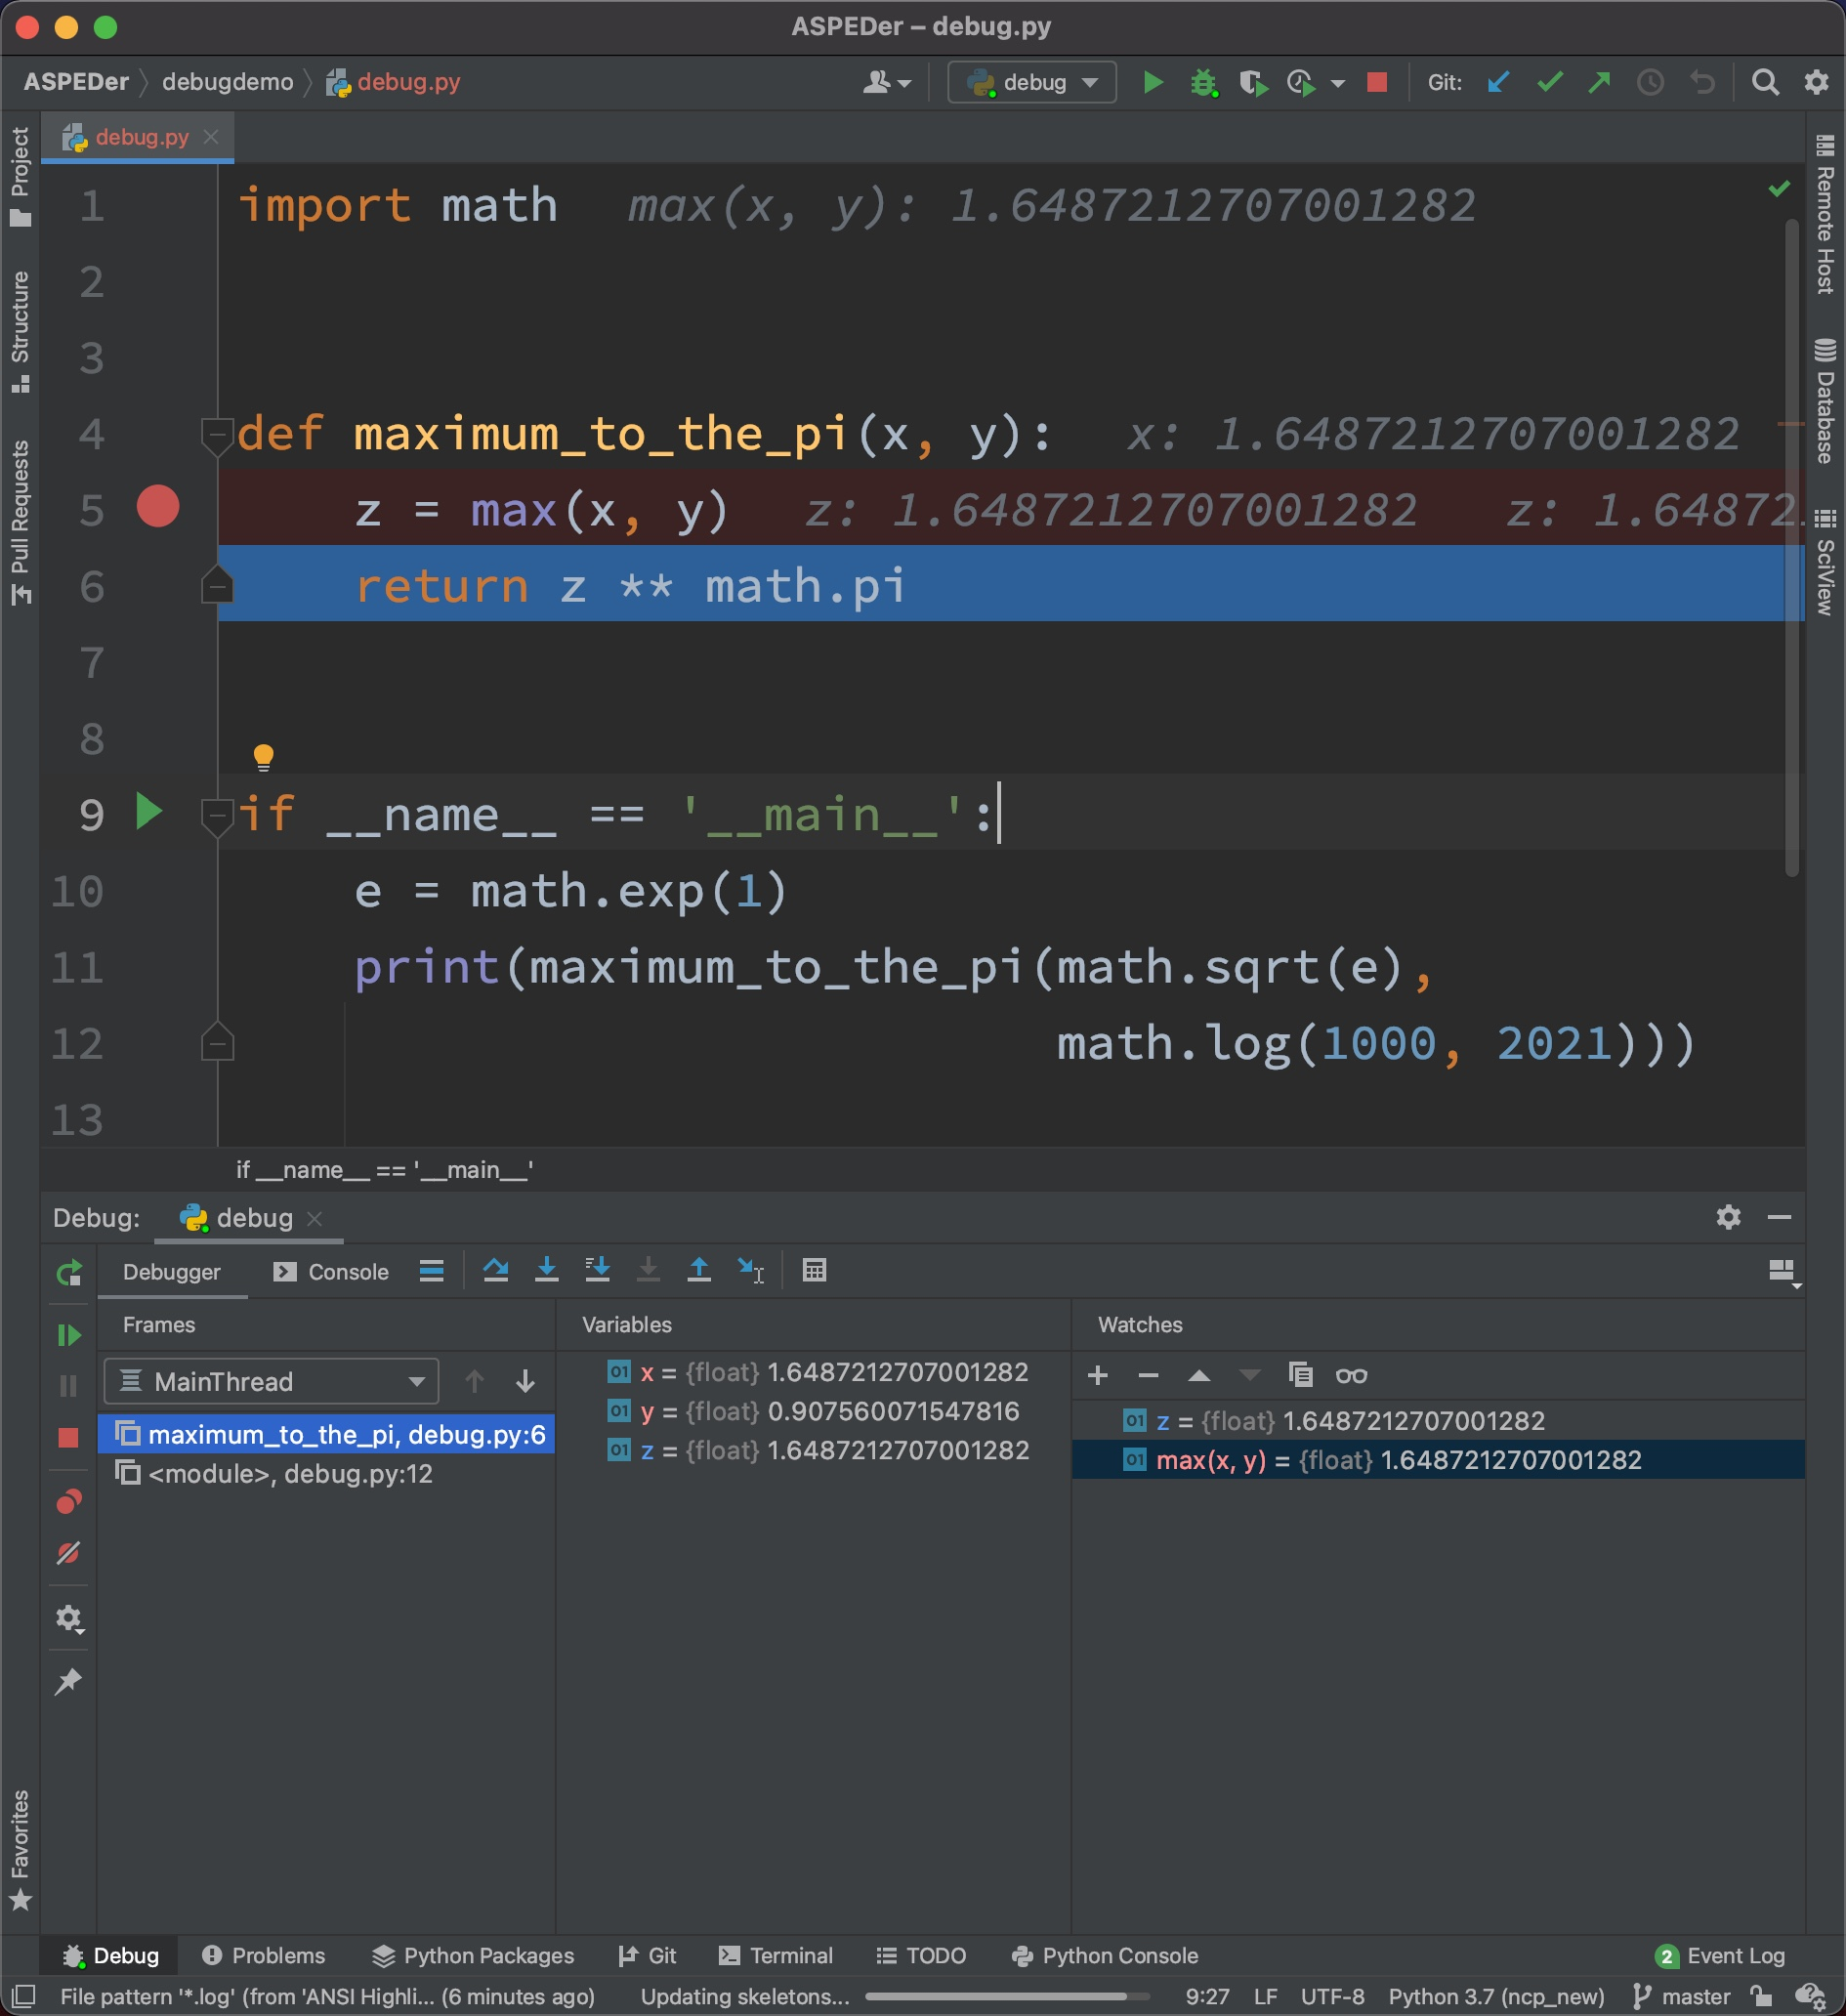
\includegraphics[height=.8\textwidth, valign=c]{figures/现代IDE调试界面.jpg}
    \caption{PyCharm调试某Python程序的界面}
    \label{fig:dbgpycharm}
\end{figure}
可以看到,对于命令式语言,由于存在明确的代码执行次序,因此调试的过程实际上是以主函数main为起点,将程序运行的过程拆解为以代码行为单位的逐条执行过程,用户通过按钮点击驱动程序向下一条执行。本文考虑将这样的调试风格应用于不一致ASP程序的调试中,通过分析ASP程序求解的特性可以发现,直接使用该方法存在两个主要的问题:
\begin{enumerate}[label=(\arabic*), topsep=0pt]
    \setlength\itemsep{-0.3em}
    \item ASP程序没有一个明确的“执行起点”;
    \item ASP程序结论的推导是规则和文字之间交错进行的,没有严格的推导顺序。
\end{enumerate}

虽然ASP程序求解时推导的过程未必严格按照某种顺序进行,但考虑其原子-规则图可以发现,当一个ASP程序确定后,无论其是否为一致性程序、回答集如何,原子-规则图可以唯一确定。进一步,若指定某个文字或规则结点为起点,对该图按照某种策略进行深度优先遍历,则能够确定一条有序的推理路径。这其中,作为起点的“某个文字或规则”,可以通过上一小节所介绍的推荐入口确定,“某种策略”是指在进行深度优先遍历时,当该结点存在多个未访问的邻接结点时,需要由用户指定访问的顺序。

解决了这两个问题后,本文通过类比,将ASP程序调试中的各要素与命令式语言调试的各要素进行一一映射,映射的结果如表\ref{tb:elementmap}所示。

\begin{table}[ht!]
    \caption{ASP程序调试与命令式语言调试要素映射表} \label{tb:elementmap}
    \centering
    \renewcommand\arraystretch{2}
    \setlength{\tabcolsep}{15mm}{
    \begin{tabular}{@{}cc@{}}
    \toprule
    命令式程序要素 & ASP程序中的要素 \\ \midrule
    \renewcommand\arraystretch{1.1}
    \begin{tabular}[c]{@{}c@{}}调试的起点函数\\ (用户设置的第一个断点)\end{tabular} & 
    \renewcommand\arraystretch{1.1}
    \begin{tabular}[c]{@{}c@{}}ARG遍历的起点结点\\ (不一致原因集合中用户选择)\end{tabular} \\
    \renewcommand\arraystretch{2}
    当前调试代码语句 & 当前遍历的ARG中的规则结点 \\
    代码中变量的值 & ARG规则结点对应规则中各文字当前真值 \\
    下一步调试的代码语句 & 下一条选中调试的规则 \\ 
    对程序中局部代码的执行 & 对ARG中各依赖边与文字真值的赋值\\
    \bottomrule
    \end{tabular}
    }
    \end{table}

    观察表\ref{tb:elementmap}可以发现,用户调试的过程实际上是在没有回答集或回答集不一致的情况下,通过交互对原子-规则图各结点与边进行标签的赋值,以构建部分解释空间,直到发现矛盾的过程,下面给出不一致ASP程序调试模型的定义。下面给出不一致ASP程序调试模型的定义。
    \begin{definition}[]
        给定一个不一致ASP程序 P,其调试模型$Dbg_{incst}(P, l, S, Q, U)$的输入包含如下五个部分:
        \begin{itemize}[topsep=0pt]
            \setlength\itemsep{-0.3em}
            \item 待调试的不一致ASP程序$P$:该程序无变量,回答集为$Lit(P)$或不一致;
            \item 调试的入口文字$l$:满足$l \in INCST(P)$,$INCST(P)$为计算得到的导致不一致的文字集合;
            \item 当前调试步$S$:定义调试中从规则节点到文字节点为一步, 文字节点到规则节点为一步,表示用户当前执行调试进行到的步数;
            \item 退出信号$Q$:表示用户在此步是否选择退出,$Q=t$表示该步骤结束后不继续调试,直接退出; $Q=f$表示该步骤结束后继续调试;
            \item 用户交互信息$U$:用户在交互过程中进行的选择,包含:
            \begin{itemize}[topsep=0pt, label=$\circ$]
                \setlength\itemsep{-0.3em}
                \item 当前步骤位于文字结点,系统无法为该文字标记真值,需要用户根据预期对该文字的真值进行指定;
                \item 当前步骤位于文字结点,该文字结点与多条规则相连接时,用户指定查看某条规则的适用推出/阻塞无法推出的路径;
                \item 当前步骤为规则结点,系统无法确定该规则是否应被适用,需要用户根据预期对该规则的适用情况进行指定;
                \item 当前步骤位于规则结点,该规则结点与多个文字相连接时,用户指定查看规则体部文字的后续推导过程。
            \end{itemize}
        \end{itemize}
        
        该模型的输出如式\eqref{eq:dbgincstmodel}所示。
        \begin{align}
            Dbg_{incst}(P, l, s, Q_s, U_s)=
            \begin{cases}
                \text{文字结点} l &s = 0, Q = f\\
                Dbg_{incst}(P, l, s-1, f, \phi) &s > 0, Q = t\\
                Dbg_{incst}(P, l, s-1, f, U_{s-1}) \cup SubExp(P, s, U_s) &s > 0, Q = f\\
                \emptyset &\text{否则}
            \end{cases}
        \end{align}\label{eq:dbgincstmodel}
    \end{definition}
    与解释模型类似,式\eqref{eq:dbgincstmodel}中仍然是递归定义的,其最核心的部分是$SubExp(P, s, U_s)$的生成,即用户选择进行下一步调试时所呈现的原子-规则子图。其中$U_s$为用户在第$s$步的交互信息,这一信息被定义为一个四元组$U_s=(UL^{true}_s, UL^{false}_s, UR^{ap}_s, UR^{bl}_s)$,为了便于算法的描述,表\ref{tb:usparameter}给出这一四元组的各元素符号表示及含义。

    \begin{table}[!ht]
        \caption{用户参数$U_s$说明}
        \centering
        \renewcommand\arraystretch{3}
        \begin{tabular}{ccc}
        \toprule \noalign{\vspace{-2ex}}
        符号 & 含义 & 取值说明 \\ \hline
        $UL^{true}_s$ & 第$s$步用户指定为真的文字集合 & \multirow{2}{*}{
        \renewcommand\arraystretch{1}    
        \begin{tabular}[c]{@{}c@{}}系统判断该步骤是否可为空,\\ 并给出一个可选文字集合,\\ 若不可为空,则从中选择\\ 一个或多个文字。\end{tabular}} \\
        $UL^{false}_s$ & 第$s$步用户指定为假的文字集合 &  \\ \hline
        $UR^{ap}_s$ & 第$s$步用户指定为适用的规则集合 & \multirow{2}{*}{
        \renewcommand\arraystretch{1}    
        \begin{tabular}[c]{@{}c@{}}系统判断该步骤是否可为空,\\ 并给出一个可选规则集合,\\ 若不可为空,则从中选择\\ 一个或多个规则。\end{tabular}} \\
        $UR^{bl}_s$ & 第$s$步用户指定为阻塞的规则集合 &  \\ \bottomrule
        \end{tabular}
        \label{tb:usparameter}
        \end{table}

    求解这一子图的过程如算法X所示。

    \begin{algorithm2e}[H]
        \label{alg:dbgSubExp}
        \DontPrintSemicolon
        \SetNoFillComment
        \SetKwInput{Initialization}{初始化}
        \SetKwInput{KwIn}{输入}
        \SetKwInput{KwOut}{输出}
        \setstretch{1.15}
        \caption{程序$P$单步调试子图生成算法}
        \KwIn{不一致ASP程序$P$,调试步$S$,用户指定的起点文字$l$,用户指定的交互信息$U_s$}
        \KwOut{单步生成的子图}
        \setcounter{AlgoLine}{0}
        \everypar={\nl}
        $ARG\_P \gets getARG(P)$ \tcp*[l]{获取程序的原子-规则图}
        $l \gets getAllNegCycles(ARG\_P)$ \tcp*[l]{获取原子规则图中的所有负环}
        \tcc{函数c$omputeIncstLitSet$返回程序$P$的不一致情形$incstCond$与导致不一致的集合$incstLit$}
        $incstCond, incstLit \gets computeIncstLitSet(P)$\;
        \eIf {$incstCond \mathrel{\mathtt{!=}} neg\_loop$}{
            \Return $incstLit$
        }
        {
            $subGraph \gets \emptyset$\;
            \ForEach{环$n\_cycle$ 在 $P$所有规则}{
                \If {$n\_cycle \cap incstLit \neq \emptyset$}{
                $subGraph \gets subGraph \cup n\_cycle$
                }
            }
            \Return $subGraph$
        }
    \end{algorithm2e}
\section{本章小结}
\chapter{参考文献}

\chapter{版权信息与更新记录}


%% ----------------------------------------------------------------------------
%%            Acknowledgement, Appendix, Bibliography and Resume
%% ----------------------------------------------------------------------------
\input{chapters/acknowledgement}
\thesisbib{seumasterthesis}
% \appendix
% \newtheorem{theorem}{定理}

\chapter{欧几里得第二定理的证明}
\label{appendix:apps}

	\begin{theorem}
		欧几里得第二定理(素数有无穷多个)\\
		证明:用反证法。假设素数有有限个($N$个),记为$p_1,p_2,\dots,p_N$。则我们构造一个新的数,
		
		\[n=p_1p_2\dots p_N+1.\]
		
		由于$p_i,i=1,2,\dots,N$为素数,则一定不为$1$。于是对于任意的$p_i,i=1,2,\dots, N$,有
		
		\[p_i\not|n\]
		
		这表明,要么$n$本身为素数,要么$n$为合数,但是存在$p_1,p_2,\dots,p_N$之外的其他素数能够将$n$进行素因子分解。不管哪种情况,都表明存在更多的素数。定理得证。\qed
	\end{theorem}

\chapter{$\sqrt{2}$是无理数的证明}
	\begin{theorem}
		$\sqrt{2}$是无理数。\\
		证明:用反证法。假设$\sqrt{2}$是有理数,则可表示为两个整数的商,即$\exists p,q, q\ne0$
		
		\[\sqrt{2}=\frac{p}{q}\]
		
		不失一般性,我们假设$p,q$是既约的,即$\gcd(p,q)=1$。对上式两边平方可得\\
		
		\begin{align*}
			2& =\frac{p^2}{q^2}\\
			p^2&=2q^2.
		\end{align*}
		
		表明$p^2$为偶数,因此$p$为偶数,记$p=2m$。则
		
		\begin{align*}
			p^2&=4m^2=2q^2\\
			q^2&=2m^2.
		\end{align*}
		
		表明$q$也为偶数,因此它们有公共因子$2$。这与它们既约的假设矛盾。定理得证。\qed
	\end{theorem} 
\resume{攻读硕士学位期间的研究成果}

\begin{enumerate}
  \renewcommand{\labelenumi}{[\theenumi].}
  \item \textbf{Hu R}, Zhang Z, Ma X, et al. Dynamic rebalancing optimization for bike-sharing system using priority-based MOEA/D algorithm[J]. IEEE Access, 2021, 9:27067-27084.
\end{enumerate}

\end{document}